%% $Id: debian-tutorial.tex,v 1.9 1999/07/01 15:44:46 jgoerzen Exp $ 

\documentclass{debian}
\usepackage[T1]{fontenc}
\usepackage[latin1]{inputenc}
\usepackage{makeidx}
\makeindex
\usepackage{graphics}
\IfFileExists{url.sty}{\usepackage{url}}{\let\url=\verb}

\makeatletter


%%%%%%%%%%%%%%%%%%%%%%%%%%%%%% LyX specific LaTeX commands.
\providecommand{\LyX}{L\kern-.1667em\lower.25em\hbox{Y}\kern-.125emX\@}
\newcommand{\noun}[1]{\textsc{#1}}
%% Special footnote code from the package 'stblftnt.sty'
%% Author: Robin Fairbairns -- Last revised Dec 13 1996
%begin{latexonly}
\let\SF@@footnote\footnote
\def\footnote{\ifx\protect\@typeset@protect
    \expandafter\SF@@footnote
  \else
    \expandafter\SF@gobble@opt
  \fi
}
\expandafter\def\csname SF@gobble@opt \endcsname{\@ifnextchar[%]
  \SF@gobble@twobracket
  \@gobble
}
\edef\SF@gobble@opt{\noexpand\protect
  \expandafter\noexpand\csname SF@gobble@opt \endcsname}
\def\SF@gobble@twobracket[#1]#2{}
%end{latexonly}

%%%%%%%%%%%%%%%%%%%%%%%%%%%%%% Textclass specific LaTeX commands.
\newenvironment{lyxcode}
  {\begin{list}{}{
    \setlength{\rightmargin}{\leftmargin}
    \raggedright
    \setlength{\itemsep}{0pt}
    \setlength{\parsep}{0pt}
    \ttfamily}%
   \item[]}
  {\end{list}}

%%%%%%%%%%%%%%%%%%%%%%%%%%%%%% User specified LaTeX commands.
\usepackage{html}
\usepackage{url}

% LaTeX Preamble from John Goerzen

% This is for a link with text.
\newcommand{\lnk}[2]{\htmladdnormallinkfoot{#1}{#2}}

%For a HTML-url (Hidden Link)
\newcommand{\hlnk}[2]{\htmladdnormallink{\texttt{#1}}{#2}}

% For an e-mail address
\newcommand{\emaillnk}[1]{\hlnk{#1}{mailto:#1}}

% Syntax: \lnk{text}{http://url.goes.here}

% For a URL with no special text, use:
% \url{http://url.goes.here}

% For a URL that goes to a *different* site online, use:
% \hlnk{foo@bar.com}{mailto:foo@bar.com}

\makeatother

\begin{document}

\pagenumbering{roman}

\vfill{}
\title{Debian GNU/Linux: Guide to Installation and Usage}
\vfill{}


\author{John Goerzen and Ossama Othman}

\maketitle
(c) 1998, 1999 Software in the Public Interest, Inc.

Permission is granted to make and distribute verbatim copies of this manual
provided the copyright notice and this permission notice are preserved on all
copies.

Permission is granted to copy and distribute modified versions of this manual
under the conditions for verbatim copying, provided also that the sections that
reprint ``The GNU General Public License'' and other clearly marked sections
held under separate copyright are reproduced under the conditions given within
them, and provided that the entire resulting derived work is distributed under
the terms of a permission notice identical to this one.

Permission is granted to copy and distribute translations of this manual into
another language under the conditions for modified versions. ``The GNU General
Public License'' may be included in a translation approved by the Free Software
Foundation instead of in the original English.

At your option, you may distribute verbatim and modified versions of this document
under the terms of the GNU General Public License, excepting the clearly marked
sections held under separate copyright.

\tableofcontents{}\listoffigures{}\listoftables{}
\newpage


\section*{Acknowledgments\index{Acknowledgments}}

% \thispagestyle{myheadings}
\markboth{Acknowledgments and Preface}{Acknowledgments and Preface}

Many people have helped with this manual. We'd like to thank everyone involved,
and we try to do that here.

Thanks to Havoc Pennington, Ardo van Rangelrooij, Larry Greenfield, Thalia Hooker,
Day Irmiter, James Treacy, Craig Sawyer, Oliver Elphick, Ivan E. Moore II, Eric
Fischer, Mike Touloumtzis, and the Linux Documentation Project for their work
on what became the Debian Tutorial document.

Thanks to Richard Stallman of the Free Software Foundation for advice and editing. 

Thanks to Bruce Perens, Sven Rudolph, Igor Grobman, James Treacy, Adam Di Carlo,
Tapio Lehtonen, and St�phane Bortzmeyer for their work on what became a collection
of installation documents.

Of course, it's impossible to thank the hundreds of Debian developers and thousands
of free software authors who gave us something to write about and use.


\section*{Preface}

\begin{quotation}
\emph{``Freedom is still the most radical idea of all.''}
\end{quotation}
This quote, penned by Nathaniel Branden, seems fitting nowhere moreso than with
the freewheeling computing industry. In the space of just a few decades, lives
the world over have been changed by computing technology. We, the people behind
the Free Software movement, are seeking to continue this trend by truly opening
up software to everyone -- not just the few people working for the companies
that write it -- but everyone. As part of this goal, this book and CD contain
a treasure chest of Free Software. Over one thousand packages, including things
such as the world's most popular web server, can be found here. You can use
this software for everything from graphic design to SQL databases.

The Free Software revolution has taken the industry by storm. Linux, started
from scratch not even 10 years ago, has been the favorite kernel of the Free
Software world. The ideas and experience gained from Free Software have truly
sent Linux and the Free Software Foundation's GNU tools all over the world.
Free systems such as Debian GNU/Linux ship with literally thousands of applications,
and they have more power and stability, and outperform some of the industry's
traditional best-selling proprietary operating systems.

Today, GNU/Linux plays a dominant role in Internet servers and among ISPs, in
academia, among computer hobbyists, and in computer science research. Debian
GNU/Linux has brought the power of Free Software to everything from laptops
to flights aboard the Space Shuttle. As I write this, companies the world over
are experiencing the joy and benefits that are Free Software. The unprecedented
power, the ability to speak directly to the people who write the software you
use, the capability to modify programs at will, and the phenomenal expertise
of the online support mechanism all combine to make Free Software a vibrant
and wonderful way to use your computing resources.

% \thispagestyle{myheadings}
\markboth{Acknowledgments and Preface}{Acknowledgments and Preface}


Starting with a Free Software such as Debian GNU/Linux can be the best thing
you've done with your computer in a long time. It's fast, powerful, stable,
versatile, and \textit{fun}!

Welcome to the revolution!\\


-- John Goerzen


\part{Guide}
\pagenumbering{arabic}
\setcounter{page}{1}


\chapter{Introduction}

\pagenumbering{arabic}
\setcounter{page}{3}


We're glad to have this opportunity to introduce you to Debian! As we begin
our journey down the road of GNU/Linux, we'd like to first talk a bit about
what exactly Debian is -- what it does, and how it fits in with the vast world
of Free Software. Then, we talk a bit about the phenomenon that is Free Software
and what it means for Debian and you. Finally, we close the chapter with a bit
of information about this book itself.


\section{What Is Debian?\label{introduction-debian}}

\textit{Debian} is a free operating system (OS) for your computer. An operating
\index{operating systems}system is the set of basic programs and utilities that make your computer run.
At the core of an operating system is the \textit{kernel}. The kernel is the
most fundamental program on the computer: It does all the basic housekeeping
and lets you start other programs. Debian uses the \textit{Linux} kernel, a
completely free piece of software started by Linus Torvalds and supported by
thousands of programmers worldwide. A large part of the basic tools that fill
out the operating system \index{GNU Project}come from the \lnk{GNU Project}{http://www.gnu.org/},
and these tools are also free.

Another facet of an operating system is application software\index{application software}\index{software!applications}: programs that
help get work done, from editing documents to running a business to playing
games to writing more software. Debian comes with more than 1,500 \textit{packages}
(precompiled software bundled up in a nice format for easy installation on your
machine) -- all for free.

The Debian system is a bit like a pyramid. At the base is Linux. On top of that
are all the basic tools, mostly from GNU. Next is all the application software
that you run on the computer; many of these are also from GNU. The Debian developers
act as architects and coordinators -- carefully organizing the system and fitting
everything together into an integrated, stable operating system: Debian GNU/Linux.

The design \index{functionality}\index{programs!functionality}\index{operating systems!functionality}philosophy of GNU/Linux is to distribute its functionality into small,
multipurpose parts. That way, you can easily achieve new functionality and new
features by combining the small parts (programs) in new ways. Debian is like
an erector set: You can build all sorts of things with it.

When you're using an operating system, you want to minimize the amount of work
you put into getting your job done. Debian supplies many tools that can help,
but only if you know what these tools do. Spending an hour trying to get something
to work and then finally giving up isn't very productive. This guide will teach
you about the core tools that make up Debian: what tools to use in certain situations
and how to tie these various tools together. 


\subsection{Who Creates Debian? }

\index{development}\index{software!development}\index{packages!development}Debian is an all-volunteer Internet-based development project. There are hundreds
of volunteers working on it. Most are in charge of a small number of software
packages and are very familiar with the software they package.

These volunteers work together by following a strict set of guidelines governing
how packages are assembled. These guidelines are developed cooperatively in
discussions on Internet mailing lists.


\section{A Multiuser, Multitasking Operating System}

As we mentioned earlier in section \ref{introduction-debian}, the design of
Debian GNU/Linux comes from the Unix operating system. Unlike common desktop
operating systems such as DOS, Windows, and MacOS, GNU/Linux\index{GNU/Linux!multiuser environment}\index{multiuser environment!GNU/Linux}\index{operating systems!GNU Linux!multiuser environment} is usually found
on large servers and \textit{multiuser\index{Multiuser}} systems. 

This means that Debian has features those other operating systems lack. It allows
a large number of people to use the same computer at once, as long as each user
has his or her own \textit{terminal\index{Terminal}.}\footnote{
A \index{terminals}\index{networks!terminals}\index{terminals!consoles}\index{consoles}\index{multitasking}\index{applications!multitasking}\index{programs!multitasking}terminal is just a keyboard and a screen that are connected to the computer
through the network, over a modem, or directly. Your keyboard and monitor form
a terminal that is directly attached to the computer: This special terminal
is often called the \textit{console}.
} To permit many users to work at once, Debian must allow many programs and applications
to run simultaneously. This feature is called \textit{multitasking}\index{Multitasking}.

Much of the power (and complexity) of GNU/Linux systems stems from these two
features. For example, the system must have a way to keep users from accidentally
deleting each other's files. The operating system also must coordinate the many
programs running at once to ensure that they don't all use the same resource,
such as a hard drive, at the same time.

If you keep in mind what Debian was originally designed to do, many aspects
of it will make a lot more sense. You'll learn to take advantage of the power
of these features.


\section{What Is Free Software? }

\index{Free Software}\index{software!Free Software}When Debian developers and users speak of ``Free Software,'' they refer to
\textit{freedom} rather than price. Debian is free in this sense: You are free
to modify and redistribute it and will always have access to the source code
for this purpose. The \lnk{Debian Free Software Guidelines}{http://www.debian.org/social\_contract\#guidelines}\index{Social Contract} describe
in more detail exactly what is meant by ``free.'' The \lnk{Free Software Foundation}{http://www.fsf.org/}\index{Free Software Foundation},
originator of the GNU Project, is another excellent source of information. You
can find a more detailed discussion of free software on the \lnk{Debian web
site}{http://www.debian.org/}\index{web sites!Debian}\index{sites!Web!Debian}\index{Debian!Web site}\index{sites!Web!Free Software Foundation}\index{Web sites!Free Software Foundation}\index{Stallman, Richard M.!Why Software Should be Free}\index{Why Software Should be Free (Stallman, Richard M.)}. One of the most well-known works in this field
is Richard M. Stallman's essay, \lnk{\emph{Why Software Should Be Free}}{http://www.fsf.org/philosophy/shouldbefree.html};
take a look at it for some insight into why we support Free Software as we do.
Recently, some people have started calling Free Software \index{Open Source Software}\index{software!Open Source}``Open Source Software'';
the two terms are interchangable.

\index{hackers}\index{comparing!crackers and hackers}\index{crackers!comparing to hackers}You may wonder why would people spend hours of their own time writing software
and carefully packaging it, only to give it all away. The answers are as varied
as the people who contribute.

\index{developing!software!free software}\index{sharing!software}\index{Hacker Ethic}Many believe in sharing information and having the freedom to cooperate with
one another, and they feel that free software encourages this. A long tradition
that upholds these values, sometimes called the Hacker\footnote{
Note that the term ``hacker'' should not be confused with the term ``cracker.''
In short, a hacker is benevolent, whereas a cracker is generally considered
malevolent. Movies and other forms of media many times incorrectly use the term
``hacker'' instead of ``cracker.''
} Ethic, started in the 1950s. The Debian GNU/Linux Project was
founded based on these Free Software ethics of freedom, sharing, and
cooperation.

Others want to learn more about computers. More and more people are looking
for ways to avoid the inflated price of proprietary software. A growing community
contributes in appreciation for all the great free software they've received
from others.

Many in academia create free software to help get the results of their research
into wider use. Businesses help maintain free software so they can have a say
in how it develops -- there's no quicker way to get a new feature than to implement
it yourself or hire a consultant to do so! Business is also interested in greater
reliability and the ability to choose between support vendors.

\index{developing!software!free software}\index{free software!developing}\index{software!free!developing}\index{sharing!software}Still others see free software as a social good, democratizing access to information
and preventing excessive centralization of the world's information infrastructure.
Of course, a lot of us just find it great fun.

\index{Social Contract}\index{developing!Free Software!Social Contract}\index{Free Software!Social Contract}\index{software!free!Social Contract}Debian is so committed to free software that we thought it would be useful if
it was formalized in a document of some sort. Our \lnk{Social Contract\index{Social Contract}}{http://www.debian.org/social\_contract}
promises that Debian will always be 100\% free software. When you install a
package from the Debian main distribution, you can be sure it meets our Free
Software Guidelines.

Although Debian believes in free software, there are cases where people want
to put proprietary software on their machine. Whenever possible Debian will
support this; though proprietary software is not included in the main distribution,
it is sometimes available on the FTP site in the \texttt{non-free} directory,
and there is a growing number of packages whose sole job is to install proprietary
software we are not allowed to distribute ourselves.

\index{comparing!software!commercial and proprietary}\index{commercial software!comparing to proprietary}\index{proprietary software!comparing to commercial}It is important to distinguish \textit{commercial} software from \textit{proprietary}
software. Proprietary software is non-free software; commercial software is
software sold for money. Debian permits commercial software, but not proprietary
software, to be a part of the main distribution. Remember that the phrase ``free
software'' does not refer to price; it is quite possible to sell free software.
For more clarification of the terminology, see \url{http://www.opensource.org/}
or \url{http://www.fsf.org/philosophy/categories.html}.


\section{About This Book}

This book is aimed at readers who are new to Debian GNU/Linux. It assumes no
prior knowledge of GNU/Linux or other Unix-like systems, but it does assume
very basic general knowledge about computers and hardware; you should know what
the basic parts of a computer are, and what one might use a computer to do.

In general, this tutorial tries to help you understand what happens inside a
Debian system. The idea is to empower you to solve new problems and get the
most out of your computer. Thus there's plenty of theory and fun facts thrown
in with the ``How To'' aspects of the manual.

We'd love to hear your comments about this book! You can reach the authors at
\emaillnk{debian-guide@complete.org}. We're especially interested in whether
it was helpful to you and how we could make it better. Whether you have a comment
or think this book is the greatest thing since sliced bread, please send us
e-mail.

Please do not send the authors technical questions about Debian, because there
are other forums for that; see Appendix \ref{docs} on page \pageref{docs}
for more information on the documentation and getting help. Only send mail regarding
the book itself to the above address.


\subsection{How to Read This Book }

The best way to learn about almost any computer program is by using it. Most
people find that reading a book without using the program isn't beneficial.
The best way to learn about Unix and GNU/Linux is by using them. Use GNU/Linux
for everything you can. Feel free to experiment!

Debian isn't as intuitively obvious as some other operating systems. You will
probably end up reading at least the first few chapters of this book. GNU/Linux's
power and complexity make it difficult to approach at first, but far more rewarding
in the long run. 

The suggested way to learn is to read a little, and then play a little. Keep
playing until you're comfortable with the concepts, and then start skipping
around in the book. You'll find a variety of topics are covered, some of which
you might find interesting. After a while, you should feel confident enough
to start using commands without knowing exactly what they do. This is a good
thing.
\tip
If you \index{programs!exiting}\index{exiting!programs}\index{applications!exiting}\index{closing!programs}ever mistakenly type a command or don't know how to exit a program,
\texttt{press~CTRL-c} (the \texttt{Ctrl} key and the lowercase letter \texttt{c}
pressed simultaneously). This will often stop the program.
\endtip


\subsection{Conventions}

\index{typographical conventions}\index{conventions!typographical}\index{modifier keys}\index{typing!modifier keys}\index{typographical conventions!modifier keys}\index{Alt key}Before going on, it's important to be familiar with the typographical conventions
used in this book.

When you should simultaneously hold down multiple keys, a notation like \texttt{CTRL-a}
will be used. This means ``press the \texttt{Ctrl} key and press lowercase letter
\texttt{a}.'' Some keyboards have both \texttt{Alt} and \texttt{Meta}; most
home computers have only \texttt{Alt}, but the \texttt{Alt} key behaves like
a \texttt{Meta} key. So if you have no \texttt{Meta} key, try the \texttt{Alt}
key instead.

\index{typographical conventions}\index{conventions!typographical}\index{modifier keys}\index{typing!modifier keys}\index{typographical conventions!modifier keys}\index{Alt key}Keys like \texttt{Alt} and \texttt{Meta} are called \textit{modifier} keys because
they change the meaning of standard keys like the letter \texttt{A}. Sometimes
you need to hold down more than one modifier; for example, \texttt{Meta-Ctrl-a}
means to simultaneously press \texttt{Meta}, \texttt{Ctrl}, and lowercase \texttt{a}. 

Some keys have a special notation -- for example, \texttt{Ret} (Return/Enter),
\texttt{Del} (Delete or sometimes Backspace), \texttt{Esc} (Escape). These should
be fairly self-explanatory.

\index{typographical conventions!spaces}\index{spaces!typographical convention}\index{conventions!typographical!spaces}Spaces used instead of hyphens mean to press the keys in sequential order. For
example, \texttt{CTRL-a~x~RET} means to simultaneously type \texttt{Ctrl} and
lowercase \texttt{a}, followed by the letter \texttt{x}, followed by pressing
\texttt{Return}. (On some keyboards, this key is labeled \texttt{Enter}. Same
key, different name.)

In sample sessions, \index{typographical conventions!bold face}\index{bold face!typographical conventions}\index{text!bold face!typographical conventions}\index{italics!typographical conventions}\index{text!italicized!typographical conventions}\index{typographical conventions!italics}bold face text denotes characters typed by the user, italicized
text denotes comments about a given part of the sample session, and all other
text is output from entering a command. For shorter commands, you'll sometimes
find that the command can be found within other text, highlighed with a monospace
font.


\chapter{Getting Started}

\begin{quotation}
``\emph{A journey of a thousand miles must begin with a single step.}'' --
Lao-Tsu
\end{quotation}
Now that you've read about the ideas and philosophy behind Linux and Debian,
it's time to start putting it on your computer! We start by talking about how
to prepare for a Debian install, then about partitioning your disk, and finally,
how to start up the installation system.


\section{Supported Hardware\index{Hardware, supported}}

Debian does not impose hardware requirements beyond the requirements of the
Linux kernel and the GNU tools.

Rather than attempting to describe all the different hardware configurations
that are supported for the PC platform, this section contains general information
and pointers to where additional information can be found.

There are two excellent places to check for detailed information: the Debian
\lnk{System Requirements}{http://www.debian.org/releases/slink/i386/ch-hardware-req.en.html}
list and the Linux Documentation Project\index{Linux Documentation Project} \lnk{Hardware Compatibility HOWTO}{http://metalab.unc.edu/LDP/HOWTO/Hardware-HOWTO.html}.
For information on video card\index{video cards!support for}\index{hardware!video cards!support for}\index{Web sites:video cards, support for}\index{sites!Web!video cards, support for} support, you may also want to look at the \lnk{XFree86}{http://www.xfree86.org/}
Project web site.


\subsection{Memory and Disk Space Requirements\index{Installation!Prerequisites}}

\index{requirements!installation!memory}\index{memory!installation requirements}\index{disk space!installation requirements}\index{RAM (Random Access Memory)!installation requirements}\index{installation!memory requirements}You must have at least 4MB of memory and 35MB of available hard disk space.
If you want to install a reasonable amount of software, including the X Window
system, and some development programs and libraries, you'll need at least 300MB.
For an essentially full installation, you'll need around 800MB.  To install
\textit{everything} available in Debian, you'll probably need around 2GB.  Actually,
installing everything doesn't make sense because some packages provide the same
services.


\section{Before You Start}

\index{installation!backups, performing}\index{backups!performing}\index{security!backups, performing}Before you start, make sure to back up every file that is now on your system.
The installation procedure can wipe out all of the data on a hard disk! The
programs used in installation are quite reliable and most have seen years of
use; still, a false move can cost you. Even after backing up, be careful and
think about your answers and actions. Two minutes of thinking can save hours
of unnecessary work.

\index{operating systems!multiple installations}\index{installations!operating systems, multiple}\index{boot loaders}\index{operating systems!boot loaders}Debian makes it possible to have both Debian GNU/Linux and another operating
system installed on the same system. If you plan to use this option, make sure
that you have on hand the original CD-ROM or floppies of the other installed
operating systems. If you repartition your boot drive, you may find that you
have to reinstall your existing operating system's boot loader\footnote{
A boot loader is responsible starting an operating system's boot procedure.
} or the entire operating system itself. 


\subsection{Information You Will Need}

If your computer is connected to a network 24 hours a day (i.e., an Ethernet
or similar LAN connection -- not a PPP connection), you should ask your network's
\index{installations!network workstations}\index{networks!workstations!installation}\index{workstations!installation}system administrator for the following information:\label{needed-info}

\begin{itemize}
\item Your host name (you may be able to decide this on your own)
\item Your domain name 
\item Your computer's IP address
\item The IP address of your network
\item The netmask to use with your network
\item The broadcast address to use on your network
\item The IP address of the default gateway system you should route to, if your network
\textit{has} a gateway
\item The system on your network that you should use as a DNS server
\item Whether you connect to the network using Ethernet
\item Whether your Ethernet interface is a PCMCIA card, and if so, the type of PCMCIA
controller you have
\end{itemize}
If your only network connection is a telephone line using PPP or an equivalent
dialup connection, you don't need to worry about getting your network set up
until your system is already installed.  See section \ref{PPP} on page \pageref{PPP}
for information on setting up PPP under Debian.  


\section{Partitioning\index{Partitioning} Your Hard Drive}

\index{arranging!hard drive}\index{installation!hard drive!partitioning}\index{organizing!hard drive}\index{hard drive!organizing}\index{partitioning!hard drive}\index{hard drive!partitioning}\index{file systems!}\index{repartitioning!hard drive}Before you install Debian on your computer, it is generally a good idea to plan
how the contents of your hard drive will be arranged. One part of this process
involves partitioning your hard drive.


\subsection{Background\label{partition-intro}}

Partitioning your disk simply refers to the act of breaking up your disk into
sections. Each section is then independent of the others. It's roughly equivalent
to putting up walls in a house; after that, adding furniture to one room doesn't
affect any other room.    

If you already have an operating system on your system (Windows 95, Windows
NT, DOS, etc.) and you want to install Debian GNU/Linux on the same disk, you
will probably need to repartition the disk. In general, changing a partition
that already has a filesystem on it will destroy any information in that filesystem.
Therefore, you should always make backups before doing any repartitioning. Using
the analogy of the house, you would probably want to move all the furniture
out of the way before moving a wall or you risk destroying your furniture. Luckily,
there is an alternative for some users; see section \ref{Lossless} on page
\pageref{Lossless} for more information.

\index{arranging!hard drive}\index{installation!hard drive! partitioning}\index{organizing!hard drive}\index{hard drive!organizing}\index{partitioning!hard drive}\index{hard drive!partitioning}\index{file systems!}\index{repartitioning!hard drive}At a bare minimum, GNU/Linux needs one partition for itself. You can have a
single partition containing the entire operating system, applications, and your
personal files. Most people choose to give GNU/Linux more than the minimum number
of partitions, however.  There are two reasons you might want to break up the
filesystem into a number of smaller partitions. The first is for safety.  If
something happens to corrupt the filesystem, generally only one partition is
affected. Thus, you only have to replace (from the backups you've been carefully
keeping) a portion of your system. At the very least, you should consider creating
what is commonly called  \index{hard drive!partitioning!root partition}\index{root partition}\index{partitioning!hard drive!root partition}a ``root partition.'' This contains the most essential
components of the system. If any other partitions get corrupted, you can still
boot into GNU/Linux to fix the system. This can save you the trouble of having
to reinstall the system from scratch.    

The second reason is generally more important in a business setting, but it
really depends on your use of the machine. Suppose something runs out of control
and starts eating disk space.  If the process causing the problem happens to
have root privileges (the system keeps a percentage of the disk away from users),
you could suddenly find yourself out of disk space. This is not good since the
operating system needs to use real files (besides swap space) for many things.
 It may not even be a problem of local origin.  For example, unsolicited e-mail
(``spam'') can easily fill a partition.  By using more partitions, you protect
the system from many of these problems. Using e-mail as an example again, by
putting the directory \texttt{/var/spool/mail} on its own partition, the bulk
of the system will work even if unsolicited e-mail fills that partition.

Another reason applies only if you have a large IDE disk drive and are using
neither LBA addressing nor overlay drivers\footnote{
See your hard drive manual for a description of these features.
}.  In this case, you will have to put the root partition into the first 1,024
cylinders of your hard drive, usually around 524 megabytes. See section \ref{disk limitations}
on page \pageref{disk limitations} for more information on this issue.

Most people feel that a swap partition\index{swap partition}\index{hard drive!partitioning!swap partition}\index{partitioning!hard drive!swap partition}\index{operating systems!swap partitions} is also a necessity, although this isn't
strictly true. ``Swap'' is scratch space for an operating system, which allows
the system to use disk storage as ``virtual memory'' in addition to physical
memory. Putting swap on a separate partition allows Linux to make much more
efficient use of it.  It is possible to force Linux to use a regular file as
swap, but this is not recommended.

The only real drawback to using more partitions is that it is often difficult
to know in advance what your needs will be. If you make a partition too small,
either you will have to reinstall the system, or you will be constantly moving
things around to make room in the undersized partition. On the other hand, if
you make the partition too big, you may be wasting space that could be used
elsewhere. \index{arranging!hard drive}\index{installation!hard drive! partitioning}\index{organizing!hard drive}\index{hard drive!organizing}\index{partitioning!hard drive}\index{hard drive!partitioning}\index{file systems}\index{repartitioning!hard drive}


\subsection{Planning Use of the System\label{disk planning}}

Disk space requirements and your partitioning scheme are influenced by the type
of installation you decide to create.

\index{profiles}\index{installation!profiles}\index{packages!profiles}For your convenience, Debian offers a number of default ``profiles'' some
of which are listed later in this section. Profiles are simply preselected sets
of packages designed to provide certain desired capabilities on your system.
Installation is easier since packages that fit your desired profile are automatically
marked for installation. Each given profile lists the size of the resulting
system after installation is complete.  Even if you don't use these profiles,
this discussion is important for planning, since it will give you a sense of
how large your partition or partitions need to be. The following are some of
the available profiles and their sizes\index{Profiles}:

\begin{description}

\index{Server profile}\item [Server\_std.]This is a small server profile, useful for a stripped-down server,
that does not have a lot of niceties for shell users.  It basically has an FTP
server, a web server, DNS, NIS, and POP. It will take up around 50MB.  Of course,
this is just the size of the software; any data you serve would be
additional.


\index{Dialup profile}\item [Dialup.]This profile would be good for a standard desktop box, including the
X Window system, graphics applications, sound, editors, etc.  The size of the
packages will be around 500MB.
\index{Work profile}\item [Work\_std.]This profile is suitable for a stripped-down user machine without
the X Window system or X applications.  It is also suitable for a laptop or
mobile computer.  The size is around 140MB.  It is possible to have a simple
laptop setup including X with less than 100MB.
\index{Devel\_comp (profile)}\item [Devel\_comp.]This is a desktop setup profile with all the popular development
packages, such as Perl, C, and C++.  It requires around 475MB.  Assuming you
are adding X and some additional packages for other uses, you should plan for
approximately 800MB of disk space for this type of installation.
\end{description}
Remember that these sizes don't include all the other materials that are normally
found, such as user files, mail, and data.  It is always best to be generous
when considering the space for your own files and data.  Notably, the Debian
\texttt{/var} directory contains a lot of state information.  The installed
package management files can easily consume 20MB of disk space. In general,
you should allocate at least 50MB for the \texttt{/var} directory because system
log files are also stored there.


\subsection{PC Disk Limitations\label{disk limitations}}

\index{PC BIOS}\index{partitioning!PC BIOS}\index{hard disk!partitioning!PC BIOS}\index{logical partitions}\index{primary partitions}\index{extended partitions}A PC BIOS generally adds additional constraints for disk partitioning. There
is a limit to how many ``primary'' and ``logical'' partitions a drive can
contain.  Additionally, there are limits to where on the drive the BIOS looks
for boot information.  More information can be found in the \lnk{Linux Partition
mini-HOWTO}{http://metalab.unc.edu/LDP/HOWTO/mini/Partition.html}. This section
will include a brief overview to help you plan most situations.

``Primary'' partitions are the original partitioning scheme for PC hard disks.
 However, there can be only four of them.  To get past this limitation, ``extended''
or ``logical'' partitions were invented.  By setting one of your primary partitions
as an extended partition, you can subdivide all the space allocated to that
partition into logical partitions. The number of logical partitions you can
create is much less limited than the number of primary partitions you can create;
however, you can have only one extended partition per drive.

\index{restrictions!partitions}\index{limitations!partitions}\index{SCSI drives!partitioning}\index{partitioning!SCSI drives}\index{boot partition}\index{partition!boot partition}\index{hard drive!partition!boot partition}Linux limits the number of partitions per drive to 15 partitions for SCSI drives
(3 usable primary partitions, 12 logical partitions), and 63 partitions for
IDE drives (3 usable primary partitions, 60 logical partitions).

The last issue you need to know about a PC BIOS is that your boot partition
-- that is, the partition containing your kernel image -- needs to be contained
within the first 1,024 cylinders of the drive.  Because the root partition is
usually your boot partition, you need to make sure your root partition fits
into the first 1,024 cylinders.

If you have a large disk, you may have to use \index{cylinder translation}\index{partitioning!cylinder translation}\index{hard drive!partitioning!cylinder translation}cylinder translation techniques,
which you can set in your BIOS, such as LBA translation mode.  (More information
about large disks can be found in the \lnk{Large Disk mini-HOWTO}{http://metalab.unc.edu/LDP/HOWTO/mini/Large-Disk.html}.)
If you are using a cylinder translation scheme, your boot partition must fit
within the \textit{translated} representation of cylinder 1,024.


\subsection{Device Names in Linux\index{Device Names}}

\index{Linux!devices}\index{devices}\index{naming!devices}Linux disks and partition names may be different from those in other operating
systems.  You should know the names that Linux uses when you create and mount
partitions. The basic scheme can be found in Table \ref{Tab: Linux Device Names}
on page \pageref{Tab: Linux Device Names}. 
\begin{table}

\caption{Linux Device Names\label{Tab: Linux Device Names}}
{\centering \begin{tabular}{|p{2in}|c|}
\hline \index{Linux!devices}\index{devices}\index{naming!devices}
Device&
Linux Name\\
\hline 
\hline 
First floppy drive&
/dev/fd0\\
\hline 
Second floppy drive&
/dev/fd1\\
\hline 
First partition on /dev/hda (typically C: in other OSs)&
/dev/hda1\\
\hline 
Fifth partition on /dev/hdc&
/dev/hdc5\\
\hline 
Second partition on /dev/sdb&
/dev/sdb2\\
\hline 
Entire Primary-Master IDE hard disk or CD-ROM&
/dev/hda\\
\hline 
Entire Primary-Slave IDE hard disk or CD-ROM&
/dev/hdb\\
\hline 
Entire Secondary-Master IDE hard disk or CD-ROM&
/dev/hdc\\
\hline 
Entire Secondary-Slave IDE hard disk or CD-ROM&
/dev/hdd\\
\hline 
First SCSI disk&
/dev/sda\\
\hline 
Second and remaining SCSI disks&
/dev/sdb and so forth\\
\hline 
First serial port (COM1 in other OSs)&
/dev/ttyS0\\
\hline 
Second, third, etc. serial ports&
/dev/ttyS1, /dev/ttyS2, etc.\\
\hline 
SCSI tape units (automatic rewind)&
/dev/st0, /dev/st1, etc.\\
\hline 
SCSI tape units (no automatic rewind)&
/dev/nst0, /dev/nst1, etc.\\
\hline 
SCSI CD-ROMs&
/dev/scd0, /dev/scd1, etc.\\
\hline 
\end{tabular}\par}\end{table}


\index{Linux!devices}\index{devices!naming}\index{naming!devices}\index{partitioning}\index{logical partitions}\index{extended partitions}The partitions on each disk are represented by appending a number to the disk
name.  For example, the names \texttt{hda1} and \texttt{hda2} represent the first and second partitions
of the first IDE disk drive in your system.    Linux represents the primary
partitions with the drive name plus the numbers 1 through 4.  For example, the
first primary partition on the first IDE drive is \texttt{/dev/hda1}. The logical
partitions are numbered starting at 5, so the first logical partition on that
same drive is \texttt{/dev/hda5}.  Remember that the extended partition -- that
\index{devices!SCSI drives!partitions}\index{SCSI drives!partitions}is, the primary partition holding the logical partitions -- is not usable by
itself.  This applies to SCSI drives as well as IDE drives.  

Let's assume you have a system with two SCSI disks, one at SCSI address 2 and
the other at SCSI address 4. The first disk (at address 2) is then named \texttt{sda}
and the second \texttt{sdb}.  If the \texttt{sda} drive has three partitions
on it, these will be named \texttt{sda1}, \texttt{sda2}, and \texttt{sda3}.
\index{controllers!SCSI!partitions, naming}The same applies to the \texttt{sdb} disk and its partitions. Note that if you
have two SCSI host bus adapters (i.e., controllers), the order of the drives
can get confusing.  The best solution in this case is to watch the boot messages, assuming you know the drive models.


\subsection{Recommended Partitioning Scheme\label{partition-scheme-recommended}}

As described above, you should have a separate smaller root partition and a
larger \texttt{/usr} partition if you have the space.  For most users, the two
partitions initially mentioned are sufficient.  This is especially appropriate
when you have a single small disk, because creating lots of partitions can waste
space.    

\index{servers!partitioning}\index{partitioning!servers}\index{networks!servers!partitioning}In some cases, you might need a separate \texttt{/usr/local} partition if you
plan to install many programs that are not part of the Debian distribution.
 If your machine will be a mail server, you may need to make \texttt{/var/spool/mail}
a separate partition.  Putting \texttt{/tmp} on its own 20 to 32MB partition,
for instance, is a good idea.  If you are setting up a server with lots of user
accounts, it's generally good to have a separate, large \texttt{/home} partition
to store user home directories.  In general, the partitioning situation varies
from computer to computer depending on its uses.    

\index{sites!Web!Multi Disk HOWTO}\index{Web sites!Multi Disk HOWTO}For very complex systems, you should see the \lnk{Multi Disk HOWTO}{http://metalab.unc.edu/LDP/HOWTO/Multi-Disk-HOWTO.html}.
It contains in-depth information, mostly of interest to people setting up servers.
   

\index{swap partitions}\index{partitioning!swap partitions}\index{devices!swap partitions}\index{hard drives!partitioning!swap partitions}\index{memory!swap partitions}Swap partition sizes should also be considered. There are many views about swap
partition sizes.  One rule of thumb that works well is to use as much swap as
you have system memory, although there probably isn't much point in going over
64MB of swap for most users. It also shouldn't be smaller than 16MB, in most
cases.  Of course, there are exceptions to these rules. If you are trying to
solve 10,000 simultaneous equations on a machine with 256MB of memory, you may
need a gigabyte (or more) of swap space.

As an example, consider a machine that has 32MB of RAM and a 1.7GB IDE drive
on \texttt{/dev/hda}. There is a 500MB partition for another operating system
on \texttt{/dev/hda1}. A 32MB swap partition is used on \texttt{/dev/hda3} and
the rest, about 1.2GB, on \texttt{/dev/hda2} is the Linux partition. 
\index{swap partitions}\index{partitioning!swap partitions}\index{devices!swap partitions}\index{hard drives!partitioning!swap partitions}\index{memory!swap partitions}


\subsection{Partitioning Prior to Installation}

\label{Lossless}\index{installation!partitioning}\index{operating systems!installation!partitioning}There are two different times that you can partition: prior to or during the
installation of Debian.  If your computer will be solely dedicated to Debian
you should partition during installation as described in section \ref{partition-create}
on page \pageref{partition-create}. If you have a machine with more than one
operating system on it, you should generally let the other operating system
create its own partitions.

The following sections contain information regarding partitioning in your native
operating system prior to Debian installation.  Note that you'll have to map
between how the other operating system names partitions and how Linux names
partitions; see Table \ref{Tab: Linux Device Names} on page \pageref{Tab: Linux Device Names}.


\subsubsection{Partitioning from DOS or Windows}

\index{installation!partitioning}\index{operating systems!installation!partitioning}\index{DOS (Disk Operating System)!partitioning}\index{Windows!partitioning}\index{repartitioning!from Windows}If you are manipulating existing FAT or NTFS partitions, it is recommended that
you use either the scheme below or native Windows or DOS tools.  Otherwise,
it is not really necessary to partition from DOS or Windows; the Linux partitioning
tools will generally do a better job.


\subsubsection{Lossless Repartitioning\index{Partition!Lossless}}

One of the most common installations is onto a system that already contains
DOS (including Windows 3.1), Win32 (such as Windows 95, 98, NT), or OS/2 and
it is desired to put Debian onto the same disk without destroying the previous
system.  As explained in section \ref{partition-intro} on page \pageref{partition-intro},
\index{hard disks!partitioning}\index{installation!partitioning}\index{operating systems!installation!partitioning}\index{DOS (Disk Operating System)!partitioning}\index{Windows!partitioning}\index{repartitioning!from Windows}decreasing the size of an existing partition will almost certainly damage the
data on that partition unless certain precautions are taken.  The method described
here, while not guaranteed to protect your data, works extremely well in practice.
 As a precaution, you should \textit{make a backup}.

Before going any further, you should have decided how you will divide up the
disk.\index{splitting!partitions}\index{dividing!partitions} The method in this section will only split a partition into two pieces.
One will contain the original operating system, and the other will be used for
Debian.  During the installation of Debian, you will be given the opportunity
to use the Debian portion of the disk as you see fit, i.e., as swap or as a
filesystem.

The idea is to move all the data on the partition to the beginning before changing
the partition information, so that nothing will be lost.  It is important that
you do as little as possible between the data movement and repartitioning to
minimize the chance of a file being written near the end of the partition as
this will decrease the amount of space you can take from the partition.

\index{tools!FIPS}\index{FIPS}\index{utilities!FIPS}The first thing you need is a copy of FIPS, which is available in the \texttt{tools}
directory on your Debian CD-ROM. This disk must be bootable. Under DOS, a bootable
floppy can be created using the command \texttt{sys~a:} for a previously formatted
floppy or \texttt{format~a:~/s} for an unformatted floppy\texttt{.} Unzip the
archive and copy the files \texttt{RESTORRB.EXE}, \texttt{FIPS.EXE} and \texttt{ERRORS.TXT}
to the bootable floppy.  \texttt{FIPS} comes with very good documentation that
you may want to read.  You should definitely read the documentation if you use
a disk compression driver or a disk manager.  Create the disk and read the documentation
\textit{before} you continue.

The next thing to be done is to move all the data to the beginning of the partition.
\texttt{DEFRAG}, which comes standard with DOS 6.0 and later, can easily do
the job.  See the FIPS documentation for a list of other software that may also
work.  Note that if you have Windows 95 or higher, you must run \texttt{DEFRAG}
from there, because DOS doesn't understand VFAT, which is used to support long
filenames in Windows 95 and higher.

After running the defragmenter (which can take a while on a large disk), reboot
with the \texttt{FIPS} floppy disk you created.  Simply type \texttt{a:\textbackslash{}
fips} and follow the directions.

\index{tools!FIPS}\index{FIPS}\index{utilities!FIPS}Note that there are many other other partition managers out there, in case \texttt{FIPS}
doesn't work for you.


\subsection{Debian Installation Steps}

As you initially install Debian, you will proceed through several
different steps: \index{hard disks!partitioning}\index{installation!partitioning}\index{operating systems!installation!partitioning}\index{DOS (Disk Operating System)!partitioning}\index{Windows!partitioning}

\begin{enumerate}
\item Boot the installation system
\item Initial system configuration
\item Install the base system
\item Boot the newly installed base system
\item Install the rest of the system
\end{enumerate}
Booting the Debian installation system, the first step, is generally done with
the Rescue Floppy or from the CD-ROM. 

Once you've booted into Linux, the \texttt{dbootstrap} program will launch and
guide you through the second step, the initial\index{system configuration}\index{packages!Debian base system}\index{Debian base system} \index{base system!configuring}\index{configuring!base system}\index{installation!base system, configuring}system configuration.  This step
is described in detail in section \ref{init-config} on page \pageref{init-config}.

The ``Debian base system'' is a core set of packages that are required to
run Debian in a minimal, stand-alone fashion. \texttt{dbootstrap} will install
it from your CD-ROM, as described in section \ref{install-base} on page \pageref{install-base}.
Once you have configured and installed the base system, your machine can ``stand
on its own.''

The final step is the installation of the remainder of the Debian system.  This
would include the applications and documents that you actually use on your computer,
such as the X Window system, editors, shells, and development environments.
The rest of the Debian system can be installed from CD-ROM. At this point, you'll
be using the standard Debian package management tools, such as \texttt{dselect}.
 This step is described in section \ref{install-packages} on page \pageref{install-packages}.


\section{Choosing Your Installation Media\index{Installation!Media}}

First, choose the boot media for the installation system.  Next, choose the
method you will use to install the base system.

To boot the installation system, you have the following choices: bootable CD-ROM,
floppies, or a non-Linux boot loader.

CD-ROM booting is one of the easiest ways to install. Not all machines can boot
directly from the CD-ROM so you may still need to use floppies. Booting from
floppies is supported for most platforms. Floppy booting is described in section
\ref{boot-from-floppies} on page \pageref{boot-from-floppies}.\index{system configuration}\index{packages!Debian base system}\index{Debian base system} \index{base system!configuring}\index{configuring!base system}\index{installation!base system, configuring}\index{CD-ROM!booting from}\index{booting!from CD-ROM}\index{Debian!booting!from CD-ROM}


\subsection{Installing from a CD-ROM\index{Installation!CD-ROM}}

If your system supports booting from a CD-ROM, you don't need any floppies.
 Put the CD-ROM into the drive, turn your computer off, and then turn it back
on. You should see a Welcome screen with a \texttt{boot} prompt at the bottom.
Now you can skip down to section \ref{installation-boot}.

If your computer didn't ``see'' the Debian CD-ROM, the easiest option is to
make two floppies for booting (described in section \ref{create-floppy}) and
then use them to start Debian. Don't worry; after Debian is finished with those
two floppies, it will find your CD-ROM with no trouble.


\subsection{Booting from Floppies\label{boot-from-floppies}\index{Installation!Floppies}}

\index{disks!floppies!booting from}\index{booting!from floppies}\index{floppies!booting from}It's not hard at all to boot from floppies. In fact, your CD-ROM contains all
the information necessary to create boot disks for you. For these instructions,
you will need to get two disks. Label the first one ``Debian 2.1 Install/Rescue
Disk'' and the second ``Debian 2.1 Modules/Drivers Disk.''


\subsubsection{Creating Floppies from Disk Images\label{create-floppy}}

\index{disks!images!writing to floppies}\index{images (disk)!writing to floppies}\index{files!disk images}\index{writing!disk images to floppies}\index{floppies!disk images!writing}\index{creating!disk images}Disk images are files containing the complete contents of a floppy disk in \textit{raw}
form.  Disk images, such as \texttt{resc1440.bin}, cannot simply be copied to
floppy drives. A special program is used to write the image files to floppy
disk in \textit{raw} mode.

First, you need to get to a DOS prompt. In Windows 95 and above, you can do
this by double-clicking on an MS-DOS icon or by going to Start\( \rightarrow  \)Programs\( \rightarrow  \)MS-DOS
prompt. Then, insert your Debian GNU/Linux CD-ROM into your CD-ROM drive. First,
you change to your CD-ROM drive. In most cases, this is D:.

\begin{lyxcode}
C:\textbackslash{}WINDOWS>\textbf{D:}
\end{lyxcode}
Now, change to the directory containing the disk images.

\begin{lyxcode}
D:\textbackslash{}>\textbf{CD~}

\textbf{\textbackslash{}DISTS\textbackslash{}SLINK\textbackslash{}MAIN\textbackslash{}DISKS-I386\textbackslash{}2.1.8-1999-02-22}
\end{lyxcode}
If you get an error, double-check what you're typing. If the error persists,
manually issue \texttt{CD~\textbackslash{}DISTS\textbackslash{}SLINK\textbackslash{}MAIN\textbackslash{}DISKS-I386},
then run \texttt{DIR}, and then \texttt{CD} into the directory
indicated.  Note that the above commands, and some other examples
below, may appear as a single line on your display even if they are
wrapped here.

Now, you're ready to create the first of two disks. Start the program to write
them out, \texttt{rawrite2}:\index{disks!images!writing to floppies}\index{images (disk)!writing to floppies}\index{files!disk images}\index{writing!disk images to floppies}\index{floppies!disk images!writing}\index{creating!disk images}

\begin{lyxcode}
D:\textbackslash{}DISTS\textbackslash{}SLINK\textbackslash{}MAIN\textbackslash{}DISKS-I386\textbackslash{}

2.1.8-1999-02-22>\textbf{rawrite2}

RaWrite~2.0~-~Write~disk~file~to~

raw~floppy~diskette
\end{lyxcode}
Rawrite2 starts and displays its welcome message. Next, it asks for the filename
and diskette drive. You tell it to write \texttt{resc1440.bin} to \texttt{a:}

\begin{lyxcode}
Enter~disk~image~source~file~name:~\textbf{resc1440.bin}

Enter~target~diskette~drive:~\textbf{a:}
\end{lyxcode}
Rawrite2 now asks you to insert a disk into the floppy drive. Do so and press
Enter.

\begin{lyxcode}
Plese~insert~a~formatted~diskette~into~

drive~A:~and~press~-ENTER-~:
\end{lyxcode}
At this point, rawrite2 will create the first of the two disks. Now, you need
to repeat the process for the second disk:

\begin{lyxcode}
D:\textbackslash{}DISTS\textbackslash{}SLINK\textbackslash{}MAIN\textbackslash{}DISKS-I386\textbackslash{}

2.1.8-1999-02-22>\textbf{rawrite2}

RaWrite~2.0~-~Write~disk~file~to

raw~floppy~diskette

Enter~disk~image~source~file~name:~\textbf{drv1440.bin}

Enter~target~diskette~drive:~\textbf{a:}

Please~insert~a~formatted~diskette~into

drive~A:~and~press~-ENTER-~:
\end{lyxcode}
By now, your disks are created. You can now use the first one to boot.


\subsubsection{Booting Debian}

\index{Debian!booting}\index{booting!Debian}\index{operating systems!Debian!booting}You are now ready to boot into Debian! Shut down your existing operating system,
turn off your computer, and place the Install/Rescue Disk into the floppy drive.
Now turn your computer back on. You should get a Welcome screen with a \texttt{boot}
prompt at the bottom.


\section{Booting the Installation System\label{installation-boot}}

You should now have the \texttt{boot} prompt. Simply press \texttt{Enter} at
this point.

Once you press \texttt{\textit{\emph{Enter}}}, you should see the message~\texttt{Loading...},
and then \texttt{Uncompressing~Linux...}, and then a screenful or so of information
about the hardware in your system. In general, you can ignore these messages.
Linux will look for various hardware devices and will tell you what it finds
and doesn't find. Don't worry about messages at this point. Just wait until
you see the Color Selection screen. If you have trouble, see section \ref{Troubleshooting the Boot Process}
on page \pageref{Troubleshooting the Boot Process}.


\chapter{Step-by-Step Installation\label{init-config}}

\index{dbootstrap}\index{programs!dbootstrap}\index{system configuration!dbootstrap}\index{applications!dbootstrap}\index{navigating!dbootstrap}\texttt{dbootstrap} is the name of the program that is run after you have booted
into the installation system.  It is responsible for initial system configuration
and the installation of the ``base system.''

The main job of \texttt{dbootstrap} and the main purpose of your initial system
configuration is to configure certain core elements of your system.  For instance,
this includes your IP address, host name, and other aspects of your networking
setup, if any.  This also includes the configuration of ``kernel modules,''
which are drivers that are loaded into the kernel.  These modules include storage
hardware drivers, network drivers, special language support, and support for
other peripherals. Configuring these fundamental things is done first, because
it is often necessary for the system to function properly for the next steps
of installation.    

\texttt{dbootstrap} is a simple, character-based application. It is very easy
to use; generally, it will guide you through each step of the installation process
in a linear fashion. You can also go back and repeat steps if you made a mistake.
Navigation within \texttt{dbootstrap} is accomplished with the arrow keys, \texttt{\textit{\emph{Enter}}},
and \texttt{\textit{\emph{Tab}}}.    


\section{Select Color or Monochrome Display}

\index{installation!monitor display!color, selecting}\index{monochrome
display!selecting}\index{selecting!monochrome display}\index{color
display!selecting}\index{selecting!color
display}\index{monitor!display color!selecting}\index{screen!display
color!selecting}\index{black-and-white display!selecting}Once the
system has finished booting, dbootstrap is invoked.  The first thing
that dbootstrap asks about is your display.  You should see the ``Select Color or
Monochrome display'' dialog box. If your monitor is capable of displaying color,
press \textit{}\texttt{\textit{\emph{Enter}}}. The display should change from
black-and-white to color.  Then press \texttt{\textit{\emph{Enter}}} again,
on the ``Next'' item, to continue with the installation.

If your monitor can display only black and white, use the arrow keys to move
the cursor to the ``Next'' menu item, and then \emph{}\textit{\emph{press}}
\texttt{\textit{\emph{Enter}}} to continue with the installation.


\section{Debian GNU/Linux Installation Main Menu\index{Installation!Menu}}

You may see a dialog box that says ``The installation program is determining
the current state of your system and the next installation step that should
be performed.'' This is a phase in which the installation program automatically
figures out what you probably need to do next. In some cases, you may not even
see this box.

\index{installation!main menu}\index{main menu!installation}\index{menus!installation}During the entire installation process, you will be presented with the main
menu, titled ``Debian GNU/Linux Installation Main Menu.'' The choices at the
top of the menu will change to indicate your progress in installing the system.
Phil Hughes wrote in the \lnk{\emph{Linux Journal}}{http://www.linuxjournal.com}
that you could teach a \textit{chicken} to install Debian! He meant that the
installation process was mostly just \textit{pecking} at the \textit{Enter}
key.  The first choice on the installation menu is the next action that you
should perform according to what the system detects you have already done.  It
should say ``Next,'' and at this point the next step in installing the system
will be taken.  


\section{Configure the Keyboard}

\index{configuring!keyboard}\index{keyboard!configuring}\index{installation!keyboard configuration}Make sure the highlight is on the ``Next'' item and press \textit{}\texttt{\textit{\emph{Enter}}}
to go to the keyboard configuration menu.

Move the highlight to the keyboard selection you desire and press \textit{}\texttt{\textit{\emph{Enter}}}.
 Use the arrow keys to move the highlight. In most cases, you can just use the
default U.S. layout.


\section{Last Chance to Back Up!}

\index{installation!disks!backing up}\index{disks!backing up}\index{backing up!disks}Did we tell you to back up your disks? Here's your first chance to wipe out
all of the data on your disks and your last chance to save your old system.
If you haven't backed up all of your disks, remove the floppy from the drive,
reset the system, and run backups.


\section{Partition a Hard Disk\label{partition-create}}

\index{hard disks!partitioning}\index{partitioning!hard disks}\index{installation!hard disks!partitioning}\index{menus!installation!Partition a Hard Disk}Whatever the ``Next'' menu selection is, you can use the down-arrow key to
select ``Partition a Hard Disk.'' Go ahead and do this now, then press \texttt{Enter}.

\index{applications!cfdisk}\index{cfdisk}\index{programs!cfdisk}\index{Linux native partition!creating}\index{Linux swap partition!creating}\index{swap partitions!Linux swap partition!creating}
The ``Partition a Hard Disk'' menu item presents you with a list of disk drives
you can partition and runs a partitioning application called \texttt{cfdisk\index{cfdisk}}.
You must create at least one ``Linux native'' (type 83) disk partition, and
you probably want at least one ``Linux swap'' (type 82) partition, as explained
in later in this section.

You will now create the partitions that you need to install Debian. For this
example, the assumption is that you are partitioning an empty hard disk.

The boot partition must reside within the first 1,024 of cylinders of your hard
disk (see section \ref{disk limitations} on page \pageref{disk limitations}).
Keeping that in mind, use the right-arrow key to highlight the ``New'' menu
selection, and then press \texttt{Enter}. You will be presented with the choice
of creating a \emph{primary} partition or a \emph{logical} partition. To help
ensure that the partition containing the boot information is within the first
1,024 cylinders, create a primary partition first. This primary partition will
be your ``Linux native'' partition. 

Highlight the ``Primary'' menu selection and press \texttt{Enter}. Next you
will need to enter how large you want that partition to be. Review section \ref{disk planning}
on page \pageref{disk planning} if you're not sure how large it should be.
Remember to leave enough space for your swap partition (see section \ref{partition-scheme-recommended}
on page \pageref{partition-scheme-recommended}). Enter the parition size you
want and then press \texttt{Enter}. Next you will be asked if you want to place
the partition at the beginning of free space or at the end. Place it at the
beginning to help ensure that it lies within the first 1,024 cylinders. Highlight
``Beginning'' and press \texttt{Enter}. At this point you will be brought
back to the main screen. Notice that the partition you created is listed. By
default, a Linux native partition was created. This partition must now be made
bootable. Make sure that the ``Bootable'' menu selection is highlighted and
press \texttt{Enter}. The partition should now have the word ``Boot'' listed
under the ``Flags'' column.

With the remaining space, create another primary partition. Using the down-arrow
key, highlight the \emph{free space} entry in the partition list. Now highlight
the ``New'' menu selection and proceed just as you did when you created the
first primary partition. Notice that the partition is listed as a Linux native
partition. Because this partition will be your swap partition, it must be denoted\index{hard disks!partitioning}\index{partitioning!hard disks}\index{installation!hard disks!partitioning}\index{menus!installation!Partition a Hard Disk}\index{applications!cfdisk}\index{cfdisk}\index{programs!cfdisk}\index{Linux native partition!creating}\index{Linux swap partition!creating}\index{swap partitions!Linux swap partition!creating}
as such. Make sure the partition you just created (your swap partition) is highlighted
and then press the left-arrow key until the ``Type'' menu selection is highlighted,
then press \texttt{Enter}. You will be presented with a list of supported partition
types. The Linux swap partition type should already be selected. If it is not,
enter the number from the list that corresponds to the Linux swap partition
(82), and then press \texttt{Enter}. Your swap partition should now be listed
as a Linux swap partition under the ``FS Type'' column in the main screen.

Your \texttt{cfdisk} screen should look something like the screenshot in Figure
\ref{Fig: cfdisk} on page \pageref{Fig: cfdisk}. The numbers may not be the
same, but the Flags and FS Type column shoulds be similar.

Until now, nothing on your disk has been altered. If you are satisfied that
the partition scheme you created is what you want, press the left-arrow key
until ``Write'' is highlighted, and press \texttt{Enter}. Your hard disk has
now been partitioned. Quit the \texttt{cfdisk} application by selecting the
``Quit'' menu selection. Once you have left \texttt{cfdisk}, you should be
back in Debian's \texttt{dbootstrap} installation application. 
\begin{figure}

\caption{\texttt{cfdisk} screenshot\label{Fig: cfdisk}}

{\par\centering \resizebox*{4in}{!}{\includegraphics{images/cfdisk.eps}} \par}
\end{figure}



\section{Initialize and Activate a Swap Partition\index{Partition!Initialization!Swap}}

\index{partitioning!swap partition!initializing}\index{swap partition!initializing}\index{initializing!swap partition}\index{hard disk!swap partition!initializing}\index{activating!swap partition}\index{installation!swap partition!initialization}This will be the ``Next'' menu item once you have created one disk partition.
You have the choice of initializing and activating a new swap partition, activating
a previously-initialized one, or doing without a swap partition.

A swap partition is strongly recommended, but you can do without one if you
insist and if your system has more than 4MB RAM. If you wish to do this, select
the ``Do Without a Swap Partition'' item from the menu and move on to the
next section.

\index{partitioning!swap partition!initializing}\index{swap partition!initializing}\index{initializing!swap partition}\index{hard disk!swap partition!initializing}\index{activating!swap partition}\index{installation!swap partition!initialization}\index{reinitializing!swap partition}\index{scanning!hard disk}\index{hard disks!scanning}\index{surface scanning!hard disks}\index{partitions!surface scanning}\index{disk blocks!scanning}It's always permissible to reinitialize a swap partition, so select ``Initialize
and Activate a Swap Partition'' unless you are sure you know what you are doing.
This menu choice will first present you with a dialog box reading ``Please
select the partition to activate as a swap device.''  The default device presented
should be the swap partition you've already set up; if so, just press \texttt{\textit{\emph{Enter}}}.
   

Next you have the option to scan the entire partition for unreadable disk blocks
caused by defects on the surface of the hard disk platters. This is useful if
you have MFM, RLL, or older SCSI disks, and it never hurts (although it can
be time-consuming).  Properly working disks in most modern systems don't require
this step, because they have their own internal mechanisms for mapping out bad
disk blocks.    

Finally, there is a confirmation message because initialization will destroy
any data previously on the partition.  If all is well, select ``Yes.''  The
screen will flash as the initialization program runs.  


\section{Initialize a Linux Partition\label{init-partition}\index{Partition!Initialization}}

\index{partitioning!Linux partition!initializing}\index{Linux partition!initializing}\index{initializing!Linux partition}\index{hard disk!Linux partition!initializing}\index{installation!Linux partition!initialization}\index{mounting!partitions}\index{partitions!mounting}\index{Linux partitions!mounting}At this point, the next menu item presented should be ``Initialize a Linux
Partition.''  If it isn't, either you haven't completed the disk partitioning
process, or you haven't made one of the menu choices dealing with your swap
partition. 

You can initialize a Linux partition, or alternately you can mount a previously
initialized one.  Note that \texttt{dbootstrap} will \textit{not} upgrade an
old system without destroying it.  If you're upgrading, Debian can usually upgrade
itself, and you won't need to use \texttt{dbootstrap}. The Debian 2.1 release
notes contain \lnk{upgrade instructions}{http://www.debian.org/releases/slink/i386/release-notes/ch-upgrading.en.html}.

If you are using old disk partitions that are not empty, i.e., if you want to
just throw away what is on them, you should initialize them (which erases all
files).  Moreover, you must initialize any partitions that you created in the
disk partitioning step.  About the only reason to mount a partition without
initializing it at this point would be to mount a partition upon which you have
already performed some part of the installation process using this same set
of installation floppies.

\index{partitioning!Linux partition!initializing}\index{Linux partition!initializing}\index{initializing!Linux partition}\index{hard disk!Linux partition!initializing}\index{installation!Linux partition!initialization}\index{mounting!partitions}\index{partitions!mounting}\index{Linux partitions!mounting}\index{hard disks!partitions!mounting}Select the ``Next'' menu item to initialize and mount the \texttt{/} disk
partition. The first partition that you mount or initialize will be the one
mounted as \texttt{/} (pronounced ``root''). You will be offered the choice
to scan the disk partition for bad blocks, as you were when you initialized
the swap partition. It never hurts to scan for bad blocks, but it could take
10 minutes or more to do so if you have a large disk.

Once you've mounted the \texttt{/} partition, the ``Next'' menu item will
be ``Install Operating System Kernel and Modules'' unless you've already performed
some of the installation steps. You can use the arrow keys to select the menu
items to initialize or to mount disk partitions if you have any more partitions
to set up. If you have created separate partitions for \texttt{/var}, \texttt{/usr},
or other filesystems, you should initialize or mount them now.


\subsection{Mount a Previously-Initialized Partition}

\index{mounting!initialized partitions}\index{partitions!mounting}\index{hard drives!partitions!mounting}An alternative to the ``Initialize a Partition'' step is the ``Mount a Previously-Initialized
Partition'' step.  Use this if you are resuming an installation that was interrupted
or if you want to mount partitions that have already been initialized.


\section{Install Operating System Kernel and Modules}

\index{operating system!kernel!installing}\index{kernel!installing}\index{installation!kernel}\index{modules!installation}This should be the next menu step after you've mounted your root partition,
unless you've already performed this step in a previous run of \texttt{dbootstrap}.
 First, you will be asked to confirm that the device you have mounted on root
is the proper one.  Next, you will be offered a menu of devices from which you
can install the kernel. Choose the appropriate device from which to install
the kernel and modules; this will either be a CD-ROM device or the first floppy
device.

If you're installing from floppies, you'll need to feed in the Rescue Floppy
(which is probably already in the drive), followed by the Drivers Floppy.


\section{Configure PCMCIA Support\index{Configuration!PCMCIA|textbf}\index{PCMCIA}}

\index{devices!PCMCIA!configuring}\index{PCMCIA!configuring}\index{configuration!PCMCIA}\index{installation!PCMCIA support!configuring}There is an alternate step, \textit{before} the ``Configure Device Driver Modules''
menu selection, called ``Configure PCMCIA Support.'' This menu is used to
enable PCMCIA support.    

If you do have PCMCIA but are not installing your Debian system using it (i.e.,
installation with a PCMCIA Ethernet card), you need not configure PCMCIA at
this point.  You can easily configure and enable PCMCIA at a later point, after
installation is complete.  However, if you are installing by way of a PCMCIA
network device, this alternate must be selected, and PCMCIA support must be
configured prior to configuring the network.    

If you need to install PCMCIA, select the alternate below ``Configure Device
Driver Modules.''  You will be asked which PCMCIA controller your system contains.
 In most cases, this will be \texttt{i82365}. In some cases, it will be \texttt{tcic};
your laptop's vendor-supplied specifications should provide the information.
 You can generally leave the next few sets of options blank.  Again, certain
hardware has special needs; the \lnk{Linux PCMCIA HOWTO}{http://metalab.unc.edu/LDP/HOWTO/PCMCIA-HOWTO.html}
contains plenty of information in case the default doesn't work.    

In some unusual cases, you may also need to modify the file \texttt{/etc/pcmcia/config.opts}.
 You can open your second virtual terminal (\texttt{\textit{\emph{Left~Alt-F2}}})
and edit the file there and then reconfigure your PCMCIA, or you can manually
force a reload of the modules using \texttt{insmod} and \texttt{rmmod}.    

Once PCMCIA is properly configured and installed, you should configure your
device drivers as described in the next section.  


\section{Configure Device Driver Modules\index{Configuration!Modules}\index{Configuration!Device drivers}}

\index{device drivers!configuring}\index{modules!device drivers!configuring}\index{installation!device drivers!configuring}\index{configuring!device drivers}Select the ``Configure Device Driver Modules'' menu item and look for devices
that are on your system. Configure those device drivers, and they will be loaded
whenever your system boots.    

You don't have to configure all your devices at this point; what is crucial
is that any device configuration required for the installation of the base system
is done here.

At any point after the system is installed, you can reconfigure your modules
with the \texttt{modconf} program.  


\section{Configure the Network\index{Network Configuration}}

\index{network!configuring}\index{configuring!network}\index{installation!network!configuring}Y\index{dbootstrap!network configuration}\index{applications!dbootstrap!network configuration}\index{programs!dbootstrap!network configuration}\index{utilities!dbootstrap!network configuration}ou'll have to configure the network even if you don't have a network, but you'll
only have to answer the first two questions -- ``Choose the Host name,'' and
``Is your system connected to a network?''


If you are connected to a network, you'll need the information you collected
from \ref{needed-info}.  However, if your primary connection to the network
will be PPP, you should choose \textit{NOT} to configure the network.    

\texttt{dbootstrap} will ask you a number of questions about your network; fill
in the answers from \ref{needed-info}. The system will also summarize your
network information and ask you for confirmation.  Next, you need to specify
the network device that your primary network connection uses.  Usually, this
will be \texttt{eth0} (the first Ethernet device).   On a laptop, it's more
likely that your primary network device is \texttt{pcmcia}.

Here are some technical details you may find handy: The program assumes the
network IP address is the bitwise \texttt{AND} of your system's IP address and
your netmask. It will guess the broadcast address is the bitwise \texttt{OR}
of your system's IP address with the bitwise negation of the netmask. It will
guess that your gateway system is also your DNS server.  If you can't find any
of these answers, use the system's guesses. You can change them once the system
has been installed, if necessary, by editing \texttt{/etc/init.d/network}. (On
a Debian system, daemons are started by scripts in the directory \texttt{/etc/init.d/}.)


\section{Install the Base System\label{install-base}\index{Base System}}

\index{base system!installation}\index{installation!base system}\index{devices!base system!installing}During the ``Install the Base System'' step, you'll be offered a menu of devices
from which you may install the base system.  Here, you need to select your CD-ROM
device.

You will be prompted to specify the path to the \texttt{base2\_1.tgz} file.
If you have official Debian media, the default value should be correct.  Otherwise,
enter the path where the base system can be found, relative to the media's mount
point.  As with the ``Install Operating System Kernel and Modules'' step,
you can either let \texttt{dbootstrap} find the file itself or type in the path
at the prompt.


\subsection{Configure the Base System\index{Configuration!Base system}\index{Base System}}

At this point you've read in all of the files that make up a minimal Debian
system, but you must perform some configuration before the system will run.
   

\index{base system!installation}\index{installation!base system}\index{devices!base system!installing}\index{installation!time zone!specifying}\index{time zone!specifying}\index{specifying!time zone}You'll be asked to select your time zone.  There are many ways to specify your
time zone; we suggest you go to the ``Directories:'' pane and select your
country (or continent).  That will change the available time zones, so go ahead
and select your geographic locality (i.e., country, province, state, or city)
in the ``Timezones:'' pane.    

\index{system clock!setting}Next, you'll be asked if your system clock is to be set to GMT or local time.
Select GMT (i.e., ``Yes'') if you will only be running Linux on your computer;
select local time (i.e., ``No'') if you will be running another operating
system as well as Debian.  Unix (and Linux is no exception) generally keeps
GMT time on the system clock and converts visible time to the local time zone.
This allows the system to keep track of daylight savings time and leap years,
and even allows a user who is logged in from another time zone to individually
set the time zone used on his or her terminal.


\subsection{Make Linux Bootable Directly from the Hard Disk}

\index{installation!master boot record}\index{master boot record!installation}If you elect to make the hard disk boot directly to Linux,  you will be asked
to install a master boot record. If you aren't using a boot manager (and this
is probably the case if you don't know what a boot manager is) and you don't
have another different operating system on the same machine, answer ``Yes''
to this question. Note that if you answer ``Yes,'' you won't be able to boot
into DOS normally on your machine, for instance.  Be careful. If you answer
``Yes,'' the next question will be whether you want to boot Linux automatically
from the hard disk when you turn on your system. This sets Linux to be the \textit{bootable
partition} -- the one that will be loaded from the hard disk.    

\index{operating systems!multiple, booting}\index{booting!operating systems!multiple}\index{multiple operating systems!booting}Note that multiple operating system booting on a single machine is still something
of a black art.  This book does not even attempt to document the various boot
managers, which vary by architecture and even by sub-architecture.   You should
see your boot manager's documentation for more information.  Remember: When
working with the boot manager, you can never be too careful.    

\index{LILO}\index{operating systems!LILO}\index{boot loaders!LILO}The standard i386 boot loader is called ``LILO.''  It is a complex program
that offers lots of functionality, including DOS, NT, and OS/2 boot management.
 To find out more about this functionality, you can read the documentation in
\texttt{/usr/doc/lilo} after your system is set up.


\section{Make a Boot Floppy}

\index{installation!boot floppies!creating}\index{boot floppies!creating}\index{floppies!boot floppies!creating}\index{disks!boot floppies!creating}You should make a boot floppy even if you intend to boot the system from the
hard disk. The reason is that it's possible for the hard disk bootstrap to be
mis-installed, but a boot floppy will almost always work. Select ``Make a Boot
Floppy'' from the menu and feed the system a blank floppy as directed. Make
sure the floppy isn't write-protected, because the software will format and
write it. Mark this the ``Custom Boot'' floppy and write-protect it once it
has been written.  


\section{The Moment of Truth    }

\index{smoke test}\index{installation!smoke test}\index{testing!installation!smoke test}\index{booting!smoke test}You system's first boot on its own power is what electrical engineers call the
``smoke test.'' If you have any floppies in your floppy drive, remove them.
 Select the ``Reboot the System'' menu item.    

If are booting directly into Debian and the system doesn't start up, either
use your original installation boot media (for instance, the Rescue Floppy)
or insert the Custom Boot floppy if you created one, and then reset your system.
 If you are \textit{not} using the Custom Boot floppy, you will probably need
to add some boot arguments.  If booting with the Rescue Floppy or similar technique,
you need to specify~\texttt{rescue~root=rootfs}, where \texttt{rootfs} is your
root partition, such as \texttt{/dev/sda1}.

Debian should boot, and you should see the same messages as when you first booted
the installation system, followed by some new messages.    


\section{Set the Root Password\label{Set the Root Password}}

\index{installation!root password!setting}\index{root password!setting}\index{passwords!root password!setting}\index{operating systems!root password!setting}\index{security!root password!setting}\index{superuser account}\index{accounts!superuser}\index{user accounts!superuser}\index{creating!accounts!superuser}The \textit{root} account is also called the \textit{superuser}; it is a login
that bypasses all security protection on your system. The root account should
be used only to perform system administration and for as short a time as possible.
   

Any password you create should contain from six to eight characters, and it
should contain both uppercase and lowercase characters, as well as punctuation
characters.  Take extra care when setting your root password, since it is such
a powerful account.  Avoid dictionary words or use of any personal information
that could be guessed.    

If anyone ever tells you he needs your root password, be extremely wary. You
should normally never give out your root account, unless you are administering
a machine with more than one system administrator.  


\section{Create an Ordinary User    }

\index{accounts!ordinary user}\index{user accounts!ordinary user}\index{ordinary user accounts}\index{creating!accounts!ordinary user}The system will ask you to create an ordinary user account.  This account should
be your main personal login.  You should \textit{not} use the root account for
daily use or as your personal login.    

Why not?  It's a lot harder to do damage to the system as an ordinary user than
as root; system files are protected. Another reason is that you might be tricked
into running a \textit{Trojan horse} program -- that is, a program that takes
advantage of your superuser powers to compromise the security of your system
behind your back. Any good book on Unix system administration will cover this
topic in more detail. Consider reading one if this topic is new to you.

\index{accounts!ordinary user}\index{user accounts!ordinary user}\index{ordinary user accounts}\index{creating!accounts!ordinary user}Name the user account anything you like.  If your name is John Smith, you might
use ``smith,'' ``john,'' ``jsmith,'' or ``js.''


\section{Shadow Password Support    }

\index{shadow passwords}\index{passwords!shadow passwords}\index{security!passwords!shadow passwords}\index{authentication!shadow passwords}Next, the system will ask whether you want to enable shadow passwords. This
is an authentication system that makes your Linux system a bit more secure.
Therefore, we recommend that you enable shadow passwords. Reconfiguration of
the shadow password system can also be done later with the \texttt{shadowconfig}
program.  


\section{Remove PCMCIA}

\index{PCMCIA!removing}\index{removing!PCMCIA}\index{kernel!PCMCIA!removing}If you have no use for PCMCIA, you can choose to remove it at this point.  This
will make your startup cleaner; also, it will make it easier to replace your
kernel (PCMCIA requires a lot of correlation between the version of the PCMCIA
drivers, the kernel modules, and the kernel itself). In general, you will not
need PCMCIA unless you're using a laptop.


\section{Select and Install Profiles}

\index{tasks}\index{applications!tasks}\index{programs!tasks}\index{utilities!tasks}\index{profiles!selecting}\index{selecting!profiles}The system will now ask you if you want to use the pre-rolled software configurations
offered by Debian. You can always choose package-by-package what you want to
install on your new machine.  This is the purpose of the \texttt{dselect} program,
described below.  But this can be a long task with the thousands of packages
available in Debian!    

So, you have the ability to choose \textit{tasks} or \textit{profiles} instead.
A \textit{task} is work you will do with the machine, such as ``Perl programming''
or ``HTML authoring'' or ``Chinese word processing.'' You can choose several
tasks. A \textit{profile} is a category your machine will be a member of, such
as ``Network server'' or ``Personal workstation.'' Unlike with tasks, you
can choose only one profile.

To summarize, if you are in a hurry, choose one profile. If you have more time,
choose the Custom profile and select a set of tasks. If you have plenty of time
and want very precise control on what is or is not installed, skip this step
and use the full power of \texttt{dselect}.    

\index{tasks}\index{applications!tasks}\index{programs!tasks}\index{utilities!tasks}\index{profiles!selecting}\index{selecting!profiles}\index{installation!tasks!selecting}\index{installation!profiles!selecting}Soon, you will enter into \texttt{dselect}. If you selected tasks or profiles,
remember to skip the ``Select'' step of \texttt{dselect}, because the selections
have already been made.    

\index{packages!selecting}\index{selecting!packages}\index{dselect}\index{applications!dselect}\index{programs!dselect}\index{utilities!dselect}A word of warning about the size of the tasks as they are displayed: The size
shown for each task is the sum of the sizes of its packages.  If you choose
two tasks that share some packages, the actual disk requirement will be less
than the sum of the sizes for the two tasks.    

Once you've added both logins (root and personal), you'll be dropped into the
\texttt{dselect} program.~\texttt{dselect} allows you to select \textit{packages}
to be installed on your system. If you have a CD-ROM or hard disk containing
the additional Debian packages that you want to install on your system, or if
you are connected to the Internet, this will be useful to you right away. Otherwise,
you may want to quit \texttt{dselect} and start it later after you have transported
the Debian package files to your system. You must be the superuser (root) when
you run \texttt{dselect}.  Information on how to use \texttt{dselect} is given
in section \ref{dselect}.


\section{Package Installation with \texttt{dselect\label{dselect}\label{install-packages}\index{dselect}}}

\index{packages!installation}\index{installation!packages}It is now time to install the software packages of your choice on your Debian
system. This is done using Debian's package management tool, \texttt{dselect}.


\subsection{Introduction       }

\index{dselect}\index{applications!dselect}\index{programs!dselect}\index{utilities!dselect}\index{packages!see also dselect}\index{selecting!packages!see also dselect}This section documents \texttt{dselect} for first-time users. It makes no attempt
to explain everything, so when you first meet \texttt{dselect}, work through
the help screens.       

\texttt{dselect} is used to select which packages you wish to install (there
are currently about 2,250 packages in Debian 2.1).  It will be run for you during
the installation. It is a very powerful and somewhat complex tool. As such,
having some knowledge of it beforehand is highly recommended. Careless use of
\texttt{dselect} can wreak havoc on your system.

\texttt{dselect} will step you through the package installation process outlined
here:
\index{installation!dselect}\index{dselect}\index{applications!dselect}\index{programs!dselect}\index{utilities!dselect}\index{packages!see also dselect}\index{selecting!packages!see also dselect}
\begin{enumerate}
\item Choose the access method to use.
\item Update list of available packages, if possible.
\item Select the packages you want on your system.
\item Install and upgrade wanted packages.
\item Configure any packages that are unconfigured.
\item Remove unwanted software.
\end{enumerate}
As each step is completed successfully, \texttt{dselect} will lead you on to
the next. Go through them in order without skipping any steps.       

Here and there in this document we talk of starting another shell. Linux has
six console sessions or shells available at any one time. You switch between
them by \textit{\emph{pressing}}~\texttt{\textit{\emph{Left~Alt-F1}}} through
\texttt{\textit{\emph{Left~Alt-F6}}}, after which you log in on your new shell
and go ahead.  The console used by the install process is the first one, a.k.a.
\texttt{tty1}, so press \texttt{\textit{\emph{Left~Alt-F1}}} when you want to
return to that process.


\subsection{Once \texttt{dselect} Is Launched       }

Once in \texttt{dselect}, you will get this screen:

\begin{lyxcode}
{\footnotesize Debian~Linux~`dselect'~package~handling~frontend.}{\footnotesize \par}

{\footnotesize 0.~~{[}A{]}ccess~~Choose~the~access~method~to~use.}{\footnotesize \par}

{\footnotesize 1.~~{[}U{]}pdate~~Update~list~of~available~packages,~if~possible.}{\footnotesize \par}

{\footnotesize 2~~~{[}S{]}elect~~Request~which~packages~you~want~on~your~system.}{\footnotesize \par}

{\footnotesize 3.~~{[}I{]}nstall~Install~and~upgrade~wanted~packages.}{\footnotesize \par}

{\footnotesize 4.~~{[}C{]}onfig~~Configure~any~packages~that~are~unconfigured.}{\footnotesize \par}

{\footnotesize 5.~~{[}R{]}emove~~Remove~unwanted~software.}{\footnotesize \par}

{\footnotesize 6.~~{[}Q{]}uit~~~~Quit~dselect.~}{\footnotesize \par}
\end{lyxcode}
Let's look at these one by one.


\subsubsection{Access\index{dselect!Access menu} }

\index{dselect}\index{applications!dselect!Access screen}\index{programs!dselect!Access screen}\index{utilities!dselect!Access screen}\index{installation!dselect!Access screen}\index{dselect!Access screen}\index{displays!dselect!Access screen}\index{Access screen!dselect}The Access screen is shown in Figure \ref{dselect access screen} on page \pageref{dselect access screen}.
\begin{figure}

\caption{\texttt{dselect} Access screen\label{dselect access screen}}

{\par\centering \resizebox*{4in}{!}{\includegraphics{images/dselect-access.eps}} \par}
\end{figure}


Here we tell \texttt{dselect} where our packages are.  Ignore the order that
these appear in.  It is very important that you select the proper method for
installation.   You may have a few more methods listed, or a few less, or you
may see them listed in a different order; just don't worry about it. In the
following list, we describe the different methods. 

\begin{description}
\index{installation!multi\_cd}\index{multi\_cd installation}\index{CDs!multi-CD installation}\index{packages!installation!multi-CD}\index{dselect!multi-CD installation}\index{applications!dselect!multi-CD installation}\index{programs!dselect!multi-CD installation}\index{utilities!dselect!multi-CD installation}\item [multi\_cd.]Quite large and powerful, this complex method is the recommended
way of installing a recent version of Debian from a set of multiple binary CDs.
Each of these CDs should contain information about the packages in itself and
all prior CDs (in the file \texttt{Packages.cd}). When you first select this
method, be sure the CD-ROM you will be using is not mounted. Place the last
\textit{binary} disk of the set (we don't need the source CDs) in the drive
and answer the questions you are asked:
\end{description}
\begin{lyxcode}
{\small CD-ROM~drive~location}{\small \par}

{\small Confirmation~that~you~are~using~a~multi-cd~set~~~}{\small \par}

{\small The~location~of~the~Debian~distribution~on~the~disk(s)}{\small \par}

{\small {[}~Possibly~{]}~the~location(s)~of~the~Packages~file(s)}{\small \par}
\end{lyxcode}
Once you have updated the available list and selected the packages to be installed,
the multi\_cd method diverges from normal procedure. You will need to run an
``install'' step for each of the CDs you have, in turn. Unfortunately, due
to the limitations of \texttt{dselect}, it will not be able to prompt you for
a new disk at each stage; the way to work for each disk is outlined here:

\begin{enumerate}
\item Insert the CD in your CD-ROM drive.
\item From the main \texttt{dselect} menu, select ``Install.''
\item Wait until \texttt{dpkg} finishes installing from this CD. (It may report installation
successful, or possibly installation errors. Don't worry about these until later.)
\item Press \texttt{Return} to go back to the main \texttt{dselect} menu.
\item Repeat with the next CD in the set.
\end{enumerate}
It may be necessary to run the installation step more than once to cover the
order of package installation; some packages installed early may need to have
later packages installed before they will configure properly.

Running a ``Configure'' step is recommended to help fix any packages that
may end up in this state. \index{installation!multi\_cd}\index{multi\_cd installation}\index{CDs!multi-CD installation}\index{packages!installation!multi-CD}

\begin{description}
\index{installation!multi-NFS, multi-mount}\index{multi-NFS, multi-mount installation}\index{CDs!multi-NFS, multi-mount installation}\index{packages!installation!multi-NFS, multi-mount}\item[multi\_nfs,~multi\_mount.]

These are similar to the multi\_cd method
and are refinements on the theme of coping with changing media -- for example,
installing from a multi\_cd set exported via NFS from another machine's CD-ROM
drive. index{dselect!multi-NFS, multi-mount installation}\index{applications!dselect!multi-NFS, multi-mount installation}\index{programs!dselect!multi-NFS, multi-mount installation}\index{utilities!dselect!multi-NFS, multi-mount installation}
\item [apt.]One of the best options for installation from a local mirror of the Debian
archive or from the network.  This method uses the ``\texttt{apt}'' system
to do complete dependency analysis and ordering, so it's most likely to install
packages in the optimal order.
\end{description}
Configuration of this method is straightforward. You may select any number of
different locations, mixing and matching \texttt{file:} URLs (local disks or
NFS mounted disks), \texttt{http:} URLs, or \texttt{ftp:} URLs.  Note, however,
that the HTTP and FTP options do not support local authenticating proxies.               

If you have proxy server for either HTTP or FTP (or both), make sure you set
the \texttt{http\_proxy} and \texttt{ftp\_proxy} environment variables, respectively.
 Set them from your shell before starting \texttt{dselect} by using the following\index{proxy servers!environment variables!setting}\index{environment variables!proxy servers!setting}\index{servers!proxy servers!environment variables, setting}
command:

\begin{lyxcode}
\#~export~http\_proxy=http://gateway:3128/

\#~dselect~\emph{}~~~~~~~~~~~~~
\end{lyxcode}

\subsubsection{Update\index{dselect!Update}}

\index{dselect!Update screen}\index{Update screen (dselect)}\index{screens!dselect!Update}\index{applications!dselect!Update screen}\index{utilities!dselect!Update screen}\index{programs!dselect!Update screen}\texttt{dselect} will read the \texttt{Packages} or \texttt{Packages.gz} files
from the mirror and create a database on your system of all available packages.
 This may take a while as it downloads and processes the files.       


\subsubsection{Select\index{dselect!Select}}

\index{Select screen (dselect)}\index{dselect!Select screen}\index{screens!dselect!Select}Hang on to your hat. This is where it all happens. The object of the exercise
is to select just which packages you wish to have installed.         

Press \texttt{\textit{\emph{Enter}}}. If you have a slow machine, be aware that
the screen will clear and can remain blank for 15 seconds. So don't start bashing
keys at this point.         

\index{installation!Help file!accessing}\index{accessing!Help file (installation)}\index{Help file (installation)!accessing}The first thing that comes up on the screen is page 1 of the Help file.  You
can get to this help by \textit{\emph{pressing}}~\texttt{\textit{\emph{?}}}
at any point in the ``Select'' screens, and you can page through the help
screens by hitting the \texttt{\textit{.}} (full stop) key.         

Before you dive in, note these points: 

\begin{itemize}
\item To exit the ``Select'' screen after all selections are complete, \textit{\emph{press}}\index{dselect!Select Screen!exiting}\index{exiting!Select screen (dselect)} \index{applications!dselect!Update screen}\index{utilities!dselect!Update screen}\index{programs!dselect!Update screen}
\texttt{\textit{\emph{Enter}}}. This will return you to the main screen if there
is no problem with your selection.  Otherwise, you will be asked to deal with
that problem. When you are happy with any given screen, press \texttt{\textit{\emph{Enter}}}
to get out.
\item Problems are quite normal and are to be expected. If you select package A and
that package requires package B to run, \texttt{dselect} will warn you of the
problem and will most likely suggest a solution. If package A conflicts with
package B (i.e., if they are mutually exclusive), you will be asked to decide
between them.
\end{itemize}
Let's look at the top two lines of the Select screen.  This header reminds us of some of the special keys listed in Table \ref{dselect keys}.

\begin{table}

\caption{Special \texttt{dselect} keys\label{dselect keys}}
\index{Select screen (dselect)}\index{dselect!Select screen}\index{screens!dselect!Select}\index{applications!dselect!Update screen}\index{utilities!dselect!Update screen}\index{programs!dselect!Update screen}\index{key combinations!dselect}
{\centering \begin{tabular}{|c|c|}
\hline 
Key&
Description\\
\hline 
\hline 
\texttt{\textbf{+}}&
Select a package for installation.\\
\hline 
\texttt{\textbf{=}}&
Place a package on hold\\
\hline 
\texttt{\textbf{-}}&
Remove a package.\\
\hline 
\texttt{\textbf{\_}}&
Remove a package and its configuration files.\\
\hline 
\texttt{\textbf{i}}, \texttt{\textbf{I}}&
Toggle/cycle information displays.\\
\hline 
\texttt{\textbf{o}}, \texttt{\textbf{O}}&
Cycle through the sort options.\\
\hline 
\texttt{\textbf{v}}, \texttt{\textbf{V}}&
A terse/verbose toggle.\\
\hline 
\end{tabular}\par}\end{table}
Table \ref{dselect package states} lists the states that \texttt{dselect} uses
to denote the status of each package it is aware of.\index{dselect!package states}\index{packages!states (dselect)}\index{states!packages (dselect)}\index{applications!dselect!package states}\index{utilities!dselect!package states}\index{programs!dselect!package states}
\begin{table}

\index{Select screen (dselect)}\index{dselect!Select screen}\index{screens!dselect!Select}
\index{applications!dselect!Update screen}
\index{utilities!dselect!Update screen}
\index{programs!dselect!Update screen}
\index{dselect!package states}
\index{packages!states (dselect)}
\index{states!packages (dselect)}
\index{applications!dselect!package states}
\index{utilities!dselect!package states}\index{programs!dselect!package states}

\caption{\texttt{dselect} Package States\label{dselect package states}}
{\centering \begin{tabular}{|c|c|c|}
\hline 
Flag&
Meaning&
Possible values\\
\hline 
\hline 
E&
Error&
Space, R, I \\
\hline 
I&
Installed State&
Space, {*}, -, U, C, I\\
\hline 
O&
Old Mark&
{*}, -, =, \_, n\\
\hline 
M&
Mark&
{*}, -, =, \_, n\\
\hline 
\end{tabular}\par}\end{table}


Rather than spell all this out here, I refer you to the Help screens where all
is revealed. One example, though.

You enter \texttt{dselect} and find a line like this: 

\begin{lyxcode}
{\scriptsize EIOM~Pri~~Section~~Package~~~Description}{\scriptsize \par}

{\scriptsize ~~{*}{*}~Opt~~misc~~~~~loadlin~~~a~loader~(running~under~DOS)~for~LINUX}{\scriptsize \par}
\end{lyxcode}
This is saying that \texttt{loadlin} was selected when you last ran \texttt{dselect}
and that it is still selected, but it is not installed. Why not? The answer
must be that the \texttt{loadlin} package is not physically available. It is
missing from your mirror.         

\index{packages!dependencies}\index{dependencies!packages}\index{built-in dependencies!packages}The information that \texttt{dselect} uses to get all the right packages installed
is buried in the packages themselves. Nothing in this world is perfect, and
it does sometimes happen that the dependencies built into a package are incorrect,
which means that \texttt{dselect} simply cannot resolve the situation.  A way
out is provided where the user can regain control; it takes the form of the
commands \texttt{\textit{\emph{Q}}} and \texttt{\textit{\emph{X}}}, which are
available in the Select screen. 

\begin{description}
\item [\texttt{Q}]An \index{overriding!package dependencies}override. Forces \texttt{dselect} to ignore the built-in dependencies
and to do what you have specified. The results, of course, will be on your own
head.              
\item [\texttt{X}]Use \texttt{\textit{\emph{X}}} if you get totally lost. It puts
things back the way they were and exits.                         
\end{description}\index{packages!dependencies}\index{dependencies!packages}\index{built-in dependencies!packages}{Select screen (dselect)}\index{dselect!Select screen}\index{screens!dselect!Select}
Keys that help you \textit{not} to get lost (!) are \texttt{\textit{\emph{R}}},
\texttt{\textit{\emph{U}}}\textit{\emph{,}} and \texttt{\textit{\emph{D}}}. 

\index{Select screen (dselect)}\index{dselect!Select screen}\index{screens!dselect!Select}\index{applications!dselect!Update screen}\index{utilities!dselect!Update screen}\index{programs!dselect!Update screen}\begin{description}
\item [\texttt{R}]Cancels all selections at this level. Does not affect selections\index{canceling!selections (dselect)}\index{packages!canceling selection (dselect)}\index{packages!selecting}\index{selecting!packages}\index{system-wide configuration!packages!selecting}
made at the previous level.            
\item [\texttt{U}]If \texttt{dselect} has proposed changes and you have made further
changes \texttt{U} will restore \texttt{dselect}'s selections.             
\item [\texttt{D}]Removes the selections made by \texttt{dselect}, leaving only yours.
                  
\end{description}
An example follows.  The \texttt{boot-floppies} package (not an example for
beginners, I know, but it was chosen because it has a lot of dependencies) depends
on these packages: 

\begin{itemize}
\item \texttt{libc6-pic}
\item \texttt{slang1-pic}
\item \texttt{sysutils}
\item \texttt{makedev}
\item \texttt{newt0.25}
\item \texttt{newt0.25-dev}
\item \texttt{popt}
\item \texttt{zlib1g}
\item \texttt{zlib1g-dev}
\item \texttt{recode}
\end{itemize}
The person maintaining \texttt{boot-floppies} also thinks that the following
packages should be installed. These are not, however, essential: 

\begin{itemize}
\item \texttt{lynx~~~}
\item \texttt{debiandoc-sgml}
\item \texttt{unzip}    
\end{itemize}

When you select boot-floppies, dselect brings up the conflict
resolution screen.  You'll notice that all the required packages have been selected.

Pressing the \texttt{\textit{\emph{R}}} key puts things back to the starting
point.

\begin{lyxcode}

{\scriptsize EIOM~Pri~Section~~Package~~~~~~Description~}{\scriptsize \par}

{\scriptsize ~~\_\_~Opt~admin~~~~boot-floppie~Scripts~to~create~the~Debian}{\scriptsize \par}

{\scriptsize ~~\_\_~Opt~devel~~~~newt0.25-dev~Developer's~toolkit~for~newt}{\scriptsize \par}

{\scriptsize ~~\_\_~Opt~devel~~~~slang1-dev~~~The~S-Lang~programming~library}{\scriptsize \par}

{\scriptsize ~~\_\_~Opt~devel~~~~slang1-pic~~~The~S-Lang~programming~library}{\scriptsize \par}
\end{lyxcode}
If you decide now that you don't want \texttt{boot-floppies}, just press \texttt{\textit{\emph{Enter}}}.

Pressing the \texttt{\textit{\emph{D}}} key puts things the way I selected them
in the first place:

\begin{lyxcode}
{\scriptsize EIOM~Pri~Section~~Package~~~~~~Description}{\scriptsize \par}

{\scriptsize ~~\_{*}~Opt~admin~~~~boot-floppie~Scripts~to~create~the~Debian}{\scriptsize \par}
\index{packages!selecting}\index{selecting!packages}\index{system-wide configuration!packages!selecting}
{\scriptsize ~~\_\_~Opt~devel~~~~newt0.25-dev~Developer's~toolkit~for~newt}{\scriptsize \par}

{\scriptsize ~~\_\_~Opt~devel~~~~slang1-dev~~~The~S-Lang~programming~library}{\scriptsize \par}

{\scriptsize ~~\_\_~Opt~devel~~~~slang1-pic~~~The~S-Lang~programming~library}{\scriptsize \par}
\end{lyxcode}
Pressing the \texttt{\textit{\noun{U}}} key restores \texttt{dselect}'s selections:

\begin{lyxcode}

{\scriptsize EIOM~Pri~Section~~Package~~~~~~Description}{\scriptsize \par}

{\scriptsize ~~\_{*}~Opt~admin~~~~boot-floppie~Scripts~to~create~the~Debian~installation}{\scriptsize \par}

{\scriptsize ~~\_{*}~Opt~devel~~~~newt0.25-dev~Developer's~toolkit~for~newt}{\scriptsize \par}

{\scriptsize ~~\_{*}~Opt~devel~~~~slang1-dev~~~The~S-Lang~programming~library}{\scriptsize \par}

{\scriptsize ~~\_{*}~Opt~devel~~~~slang1-pic~~~The~S-Lang~programming~library}{\scriptsize \par}
\end{lyxcode}

I suggest running with the defaults for now; you will have ample opportunities
to add more later.

Whatever you decide, press \texttt{\textit{\emph{Enter}}} to accept and return
to the main screen. If this results in unresolved problems, you will be bounced
right back to another problem resolution screen.

The \texttt{\textit{\emph{R}}}, \texttt{\textit{\emph{U}}}, and \texttt{\textit{\emph{D}}}
keys are very useful in ``what if'' situations. You can experiment at will
and then restore everything and start again. \textit{Don't} look on them as
being in a glass box labeled ``Break in Case of Emergency.''

After making your selections in the Select screen, press \texttt{\textit{\emph{I}}}
to give you a big window, press \texttt{\textit{\emph{t}}} to take you to the
beginning, and then use the \texttt{\textit{\emph{Page~Down}}} key to look quickly
through the settings. This way you can check the results of your work and spot
glaring errors. Some people have deselected whole groups of packages by mistake
and not noticed the error until too late. \texttt{dselect} is a \textit{very}
powerful tool; don't misuse it.

You should now have the situation shown in Table \ref{pre-install package category states}.\index{packages!selecting}\index{selecting!packages}\index{system-wide configuration!packages!selecting}

\begin{table}

\caption{Expected Package Category States\label{pre-install package category states}}
{\centering \begin{tabular}{|c|c|}
\hline 
Package category&
Status\\
\hline 
\hline 
Required&
all selected \\
\hline 
Important&
all selected\\
\hline 
Standard&
mostly selected\\
\hline 
Optional&
mostly deselected\\
\hline 
Extra&
mostly deselected\\
\hline 
\end{tabular}\par}\end{table}


Happy? Press \texttt{\textit{\emph{Enter}}} to exit the Select process. You
can come back and run Select again if you wish.       


\subsubsection{Install}

\index{installing!packages}\index{packages!installing}\index{dselect!packages!installing}\index{utilities!dselect!packages, installing}\index{programs!dselect!packages, installing}\texttt{dselect} runs through the entire set of packages and installs those
selected.  Expect to be asked to make decisions as you go. It is often useful
to switch to a different shell to compare, say, an old configuration with a
new one.  If the old file is \texttt{conf.modules}, the new one will be \texttt{conf.modules.dpkg-dist}.

The screen scrolls past fairly quickly on a fast machine. You can stop and start
it with \texttt{\textit{\emph{Ctrl-s}}} \textit{\emph{and}}~\texttt{\textit{\emph{Ctrl-q}}},
respectively, and at the end of the run, you will get a list of any uninstalled
packages. 

It can happen that a package does not get installed because it depends on some
other package that is listed for installation but is not yet installed. The
answer here is to run Install again.  Cases have been reported where it was
necessary to run it four times before everything slipped into place.  This will
vary by your acquisition method. \index{installing!packages}\index{packages!installing}\index{dselect!packages!installing}\index{utilities!dselect!packages, installing}\index{programs!dselect!packages, installing}     


\subsubsection{Configure}

Most packages get configured in step 3, but anything left hanging can be configured\index{configuring!packages}\index{packages!configuring}\index{dselect!packages!configuring}\index{utilities!dselect!packages, configuring}\index{programs!dselect!packages, configuring}
here.       


\subsubsection{Remove}

Removes packages that are installed but no longer required.       


\subsubsection{Quit}

I suggest running \texttt{/etc/cron.daily/find} at this point, because you have
a lot of new files on your system. Then you can use \texttt{locate} to get the
location of any given file.


\subsection{A Few Hints in Conclusion}

When the install process runs \texttt{dselect} for you, you will doubtless be
eager to get Debian running as soon as possible. Well, please be prepared to
take an hour or so to learn your way around and then get it right. When you
enter the Select screen for the first time, don't make \emph{any} selections
at all -- just press \texttt{\textit{\emph{Enter}}} and see what dependency
problems there are. Try fixing them. If you find yourself back at the main screen,
run Select again.

You can get an idea of the size of a package by \textit{\emph{pressing}}~\texttt{\textit{\emph{i}}}
\textit{\emph{twice}} and looking for the ``Size'' figure. This is the size
of the compressed package, so the uncompressed files will be a lot bigger (see
``Installed-Size,'' which is in kilobytes, to know it).       

Installing a new Debian system is a complex thing, but \texttt{dselect} can
do it for you as easy as can be. So take the time to learn how to drive it.
Read the help screens and experiment with \texttt{i}\textit{,}~\texttt{I}\textit{,}
\texttt{o}\textit{,} and \texttt{O}. Use the \texttt{R} key. It's all there,
but it's up to you to use it effectively.


\section{Glossary}

The following terms will be useful to you throughout this book and in general
when you're talking about Debian.

\begin{description}
\index{glossary}\index{packages}\item [Package.]A file that contains everything needed to install, de-install, and
run a particular program. The program that handles packages is \texttt{dpkg}.
\texttt{dselect} is a front-end to \texttt{dpkg}. Experienced users often use
\texttt{dpkg} to install or remove a package.
\item [Package~names.]All package names have the form xxxxxxxxxxx.deb. Sample package
names include the following:
\end{description}
\begin{itemize}
\item \texttt{efax\_08a-1.deb}
\item \texttt{lrzsz\_0.12b-1.deb}
\item \texttt{mgetty\_0.99.2-6.deb}
\item \texttt{minicom\_1.75-1.deb}
\item \texttt{term\_2.3.5-5.deb}
\item \texttt{uucp\_1.06.1-2.deb}
\item \texttt{uutraf\_1.1-1.deb}
\item \texttt{xringd\_1.10-2.deb}
\item \texttt{xtel\_3.1-2.deb}
\end{itemize}

\chapter{Logging In}

Your system is now installed! Pat yourself on the back for a job well done!
Now it's time to start using the system. In this chapter, we introduce you to
the Debian command line, some security principles, and how to exit the system.
In later chapters, we'll go into more detail on these topics and introduce you
to the Debian graphical interface, X11.


\section{First Steps}

\index{logging in}\index{user accounts!logging in}\index{accounts!user!logging in}\index{passwords!logging in}\index{security!passwords!logging in}After you quit \texttt{dselect}, you'll be presented with the \texttt{login:}
prompt.  You can now log in using the personal login and password you selected;
your system is now ready to use. Let's examine what it means to log in and how
this process works.

To use Debian, you must identify yourself to the system. This is so it knows
who you are, what you have permission to do, and what your preferences are. 

To this end, you have a \textit{username} or \textit{login}. If you installed
Debian yourself, you should have been asked to give such a name during installation.
If you are logging on to a system administered by someone else, you'll have
to ask him for an account on the system and a corresponding username.

You also have a password, so no one else can pretend to be you. If you don't
have a password, anyone can log on to your computer from the Internet and do
bad things. If you're worried about security, you should have a password.

Many people prefer to trust others not to do anything malicious with their account;
hopefully your work environment doesn't encourage paranoia. This is a perfectly
reasonable attitude; it depends on your personal priorities and your environment.
Obviously a home system does not need to be as secure as a military installation.
Debian allows you to be as secure or as insecure as you like. 

\index{logging in}\index{user accounts!logging in}\index{accounts!user!logging in}\index{passwords!logging in}\index{security!passwords!logging in}When you start Debian, you'll see a \textit{prompt}: a request from the computer
for some information. In this case, the prompt is \texttt{login:}. 

You should type your username and, when requested, your password. The password
does not appear on the screen as you type it. Press \texttt{Enter} after both
the username and the password. If you type your username or password incorrectly,
you'll have to start over. 

If you do it correctly, you'll see a brief message and then a \texttt{\$} prompt.
The \texttt{\$} is printed by a special program called the \textit{shell} and
is thus called a \textit{shell prompt}\index{prompts!shell prompts}. This is where you give commands to the
system. 

\index{shell commands!typing}\index{typing!shell commands}\index{commands!shell commands!typing}Try entering the command \texttt{whoami} now. There is a \textit{cursor} to
the right of the shell prompt. Your cursor is a small underscore or rectangle
that indicates where you're typing; it should move as you type. Always press
\texttt{Enter} when you're done typing a shell command. 

\texttt{whoami} tells your username. You'll then get a new shell prompt. 

For the rest of the book, when we say to enter a command, you should type it
at the shell prompt and press the \texttt{Enter} key.

When you're done working, you may want to log out of the system. To exit the
shell, enter the \texttt{exit} command. Keep in mind that if you remain logged
in, someone could come along and use your account. Hopefully you can trust those
in your office or home not to do this; but if you do not trust your environment,
you should be certain to log out when you leave.


\section{Command History and Editing the\\Command Line\index{Comand Line!History}\index{History|see{Command Line History}}}

Whatever you type after the shell prompt and before pressing \texttt{Enter}
is called a \textit{command line}. It's a line of text that commands the computer
to do something. \index{command line}\index{shell prompt!command line}\index{typing!command line}The Debian default shell offers several features to make entering
command lines easy.

\index{command line}\index{shell prompt!command line}\index{typing!command line}\index{scrolling!commands}\index{command history}\index{shell prompt!command history}You can scroll up to previous commands to run them again, or you can modify
them slightly and \textit{then} run them again. Try this: Enter any command,
such as \texttt{whoami}; then press the \texttt{Up~Arrow} key. The \texttt{whoami}
command will reappear at the prompt. You can then press \texttt{Enter} to run
\texttt{whoami} a second time.

If you've entered several commands, you can keep pressing the \texttt{Up~Arrow}
key to go back through them. This feature is handy if you're doing the same
thing several times, or if you type a command incorrectly and want to go back
to fix it. You can press the \texttt{Down~Arrow} key to move in the other direction,
toward your more recent commands. If there are no more commands to move to,
the computer will beep.

You can also move around on the command line to make changes. The easiest way
is with the \texttt{Left} and \texttt{Right~Arrow} keys. Try typing \texttt{whoasmi}
instead of \texttt{whoami}, and then use the \texttt{Left~Arrow} key to move
back to the \texttt{s}. You can erase the \texttt{s} with the \texttt{Backspace}
or \texttt{Delete} keys.

There are more advanced features as well (no need to memorize them all now,
though). Try pressing \texttt{Ctrl-a}. This moves you to the beginning of the
line. \texttt{Ctrl-k} (the \texttt{k} stands for ``kill'') deletes all characters
until the end of the line; try it from the middle of the command line. Using
\texttt{Ctrl-a} followed by \texttt{Ctrl-k}, you can delete the entire command
line. \texttt{Ctrl-y} pastes the last thing you killed, reinserting it at the
current cursor position (\texttt{y} stands for ``yank,'' as in ``yank it
back''). \texttt{Ctrl-e} will move the cursor to the end of the command line.

Go ahead and play around with command-line editing to get a feel for it. Experiment.


\section{Working as Root\label{Working as root}}

\index{root user}\index{accounts!root user}\index{security!root user}\index{user accounts!root user}\index{superuser}Because Debian is a multiuser system, it's designed to keep any one user or
program from breaking the entire system. The kernel will not allow normal users
to change important system files. This means that things stay the way they're
supposed to, safe from accidents, viruses, and even malicious pranks. Unlike
other operating systems, Debian is safe from these threats. You won't need an
anti-virus program. 

However, sometimes you need to change important system files; for example, you
might want to install new software or configure your network connection. To
do so, you have to have greater powers than a normal user; you must become the
\textit{root user} (also called the \textit{superuser}). 

To become root, just log on with the username \texttt{root} and the root password;
this was set during installation, as described in section \ref{Set the Root Password}
on page \pageref{Set the Root Password}.\index{root user}\index{accounts!root user}\index{security!root user}\index{user accounts!root user}\index{superuser}\index{passwords!superuser}

At many sites, only the system administrator has the root password, and only
the system administrator can do the things that one must be root to do. If you're
using your own personal computer, \textit{you} are the system administrator,
of course. If you don't have root privileges, you will have to rely on your
system administrator to perform any tasks that require root privileges.

Sometimes you'll have the root password even on a shared corporate or educational
server, because the system administrator trusts you to use it properly. In that
case, you'll be able to help administer the system and customize it for your
needs. But you should be sure to use the password responsibly, respecting other
users at all times. 

If you have the password, try logging on as root now. \index{whoami command}\index{commands!whoami}Enter the \texttt{whoami}
command to verify your identity. Then \textit{log out immediately}. When you're
root, the kernel will not protect you from yourself, because root has permission
to do anything at all to the system. Don't experiment while you're root. In
fact, don't do anything as root unless absolutely necessary. This isn't a matter
of security, but rather of stability. Your system will run much better if it
can keep you from making mistakes. 

You may find the \texttt{su} command more convenient than logging in as root.
su allows you to assume the identity of another user, usually root unless you
specify someone else. (You can remember that su stands for Super User, though
some say it stands for Set UserID.) 

Here's something to try. Log on as yourself -- that is, not as root. Then your
session will look something like the one in Figure \ref{Fig: Sample Session with su}.\index{su command}\index{commands!su}

When you're doing system administration tasks, you should do as much as possible
as yourself. Then use \texttt{su}, do the part that requires root privileges,
and use the \texttt{exit} command to turn off privileges so you can no longer
harm anything. 

You can use \texttt{su} to assume the identity of any user on the system, not
just root. To do this, type \texttt{su}~\texttt{\emph{user}} where \emph{user}
is the user you want to become. You'll have to know the user's password, of
course, unless you're root at the time or the user has no password. 

\begin{figure}

\caption{Sample session with \texttt{su\label{Fig: Sample Session with su}}}

\begin{lyxcode}
\$~\textbf{whoami~~~~~~~~~~~~}\textrm{\textit{Check your current username}}

username~~~~~~~~~~~~\textrm{\textit{This will show your username}}

\$~\textbf{su~~~~~~~~~~~~~~~~}\textrm{\textit{Ask system for superuser access}}

Password:~~~~~~~~~~~\textrm{\textit{Type your root password here}}

machine:\~{}\#~\textbf{whoami}

root~~~~~~~~~~~~~~~~\textrm{\textit{You're now on as root}}

machine:\~{}\#~\textbf{exit~~~~} \textrm{\textit{Exit your root shell}}

\$~\textbf{exit~~~~~~~~~~~~~~}\textrm{\textit{Exit your ``normal'' shell}}\end{lyxcode}
\end{figure}



\section{Virtual Consoles\index{Virtual Consoles}}

\index{virtual consoles}\index{kernel!virtual consoles}\index{Linux!kernel!virtual console}\index{networks!virtual console}\index{consoles!virtual consoles}\index{multiuser environments!virtual console}The Linux kernel supports \textit{virtual consoles}. These provide a way of
making your single screen and keyboard seem like multiple terminals that are
connected to the same system. Thankfully, using virtual consoles is one of the
simplest things about Debian: There are ``hot keys'' for switching among the
consoles quickly. To try it, log in to your system and press \texttt{Alt-F2}
(simultaneously press the left \texttt{Alt} key, and \texttt{F2}, that is, function
key number 2).

You should find yourself at another login prompt. Don't panic: You are now on
virtual console (VC) number 2! Log in here and do some things -- more \texttt{whoami}
commands or whatever -- to confirm that this is a real login shell. Now you
can return to virtual console number 1 by pressing \texttt{Alt-F1}. Or you can
move on to a \textit{third} virtual console, in the obvious way (\texttt{Alt-F3}).

Debian comes with six virtual consoles enabled by default, which you access
with the \texttt{Alt} key and function keys \texttt{F1} through \texttt{F6}.
(Technically, there are more virtual consoles enabled, but only six of them
allow you to log in. The others are used for the X Window system or other special
purposes.)

If you're using the X Window system, it will generally start up on the first
unused virtual console -- probably VC 7. Also, to switch from the X virtual
console to one of the first six, you'll have to add \texttt{Ctrl} to the key
sequence. So that's \texttt{Ctrl-Alt-F1} to get to VC 1. But you can go from
a text VC to the X virtual console using only \texttt{Alt}. If you never leave
X, you won't have to worry about this; X automatically switches you to its virtual
console when it starts up. 

Once you get used to them, virtual consoles will probably become an indispensable
tool for getting many things done at once. (The X Window system serves much
the same purpose, providing multiple windows rather than multiple consoles.)
You can run a different program on each VC or log on as root on one VC and as
yourself on another. Or everyone in the family can use his or her own VC; this
is especially handy if you use X, in which case you can run several X sessions
at once on different virtual consoles. \index{virtual consoles}\index{kernel!virtual consoles}\index{Linux!kernel!virtual console}\index{networks!virtual console}\index{consoles!virtual consoles}\index{multiuser environments!virtual console}


\section{Shutting Down\index{Shutdown}\label{shutdown}}

\textit{Do not just turn off the computer! You risk losing valuable data!}

\index{shutting down}\index{Linux!kernel!disk cache}\index{disk cache}\index{RAM!disk cache}\index{memory!disk cache}\index{APM (Advanced Power Management)}If you are the only user of your computer, you might want to turn the computer
off when you're done with it. 

To avoid possibly weakening some hardware components, only turn off the computer
when you're done for the day. Power up and power down are the two greatest contributors
to wear and tear on computer components. Turning the computer on and off once
a day is probably the best compromise between your electric bill and your computer's
lifespan.

It's a bad thing to just press the power switch when you're done using the computer.
It is also bad to reboot the machine (with the Reset button) without first taking
proper precautions. The Linux kernel, in order to improve performance, has a
\textit{disk cache}. This means it temporarily stores information meant for
permanent storage in RAM. Because memory is thousands of times faster than a
disk, this makes many file operations move more quickly. Periodically, the information
Linux has in memory is actually written to the disk. This is called \textit{syncing}.
In order to turn off or reboot the computer safely, you'll have to tell the
computer to clear everything out of memory and put it in permanent storage.

To reboot, just type \texttt{reboot} or press \texttt{Ctrl-Alt-Del} (that's
\texttt{Ctrl}, \texttt{Alt}, and \texttt{Delete}).

To shut down, you'll have to log in as \texttt{root}. As root, just type the
command \texttt{shutdown~-h~now}. The sytem will go through the entire shutdown
procedure, including the \texttt{sync} command, which clears the disk cache
as described above. When you see \texttt{System~halted}, it's safe to turn off
the computer. If you have Advanced Power Management (APM) support in your kernel
and BIOS, the computer might shut itself off and save you the trouble. APM is
common in laptops\index{APM} and is also found in certain desktop mainboards.


\chapter{The Basics}

It's now time to explore the system in more detail. You've seen how to log in
and shut down the system. In this chapter, we explore the Linux comand line,
how Linux deals with files and directories, and some basics on identifying yourself
to others.


\section{The Command Line and Man Pages\index{Command Line|textbf}\label{man pages}}

We've already discussed the \textit{\emph{command line}} -- that is, commands
you type after the shell prompt. This section describes the structure of more
complicated command lines. \index{man pages}

\index{structure!command line}\index{command line!structure}\index{commands!parameters}\index{parameters}\index{options (commands)}\index{arguments}\index{commands!arguments}A minimal command line contains just a command name, such as \texttt{whoami}.
But other things are possible. For example, you might type: \texttt{man~whoami}.
This command requests the online manual for the \texttt{whoami} program (you
may have to press the space bar to scroll through the documentation or press
\texttt{q} to quit). A more complicated example is \texttt{man~-k~PostScript}.
This command line has three parts. It begins with the command name, \texttt{man}.
Then it has an \textit{option} or \textit{switch}, \texttt{-k}, followed by
an \textit{argument}, \texttt{PostScript}. Some people refer to everything except
the command name as the \textit{parameters} of the command. So, options and
arguments are both parameters. 

Options change the behavior of a command, switching on particular features or
functionality. They usually have a \texttt{-} before them. The \index{long form!options}\index{syntax!commands}GNU utilities
also have ``long forms'' for the options; the long form of \texttt{-k} is
\texttt{-{}-apropos}. You can enter \texttt{man~-h} or \texttt{man~-{}-help}
to get a full list of options for the \texttt{man} command. Every command will
have its own set of options, though most have \texttt{-{}-help} and \texttt{-{}-version}
options. Some commands, such as \texttt{tar}, do not require the ``\texttt{-}''
before their options for historical reasons. 

Anything that isn't an option and isn't the command name is an \textit{argument}
(in this case, \texttt{PostScript}). Arguments can serve many purposes; most
commonly, they are filenames that the command should operate on. In this case,
\texttt{PostScript} is the word you want \texttt{man} to search for. In the
case of \texttt{man~whoami}, the argument was the command you wanted information
about. 

Here's a breakdown of the \texttt{man~-k~PostScript} command line: 

\begin{description}
\item [\texttt{man}.]The command name, tells the computer to look at the manual pages.
These provide documentation for commands. For example, \texttt{man~whoami} will
give you documentation on the \texttt{whoami} command. 
\item [\texttt{-k}.]The option, changes the behavior of \texttt{man}. Normally \texttt{man}
expects a command name, such as \texttt{whoami}, for an argument and looks for
documentation of that command. But with the \texttt{-k} or \texttt{-{}-apropos}
option, it expects the argument to be a keyword. It then gives a list of all
manual pages with that keyword in their description. 
\item [\texttt{PostScript}.]is the argument; because we used the \texttt{-k} option,
it's the keyword to search for. 
\end{description}
\texttt{-k} and \texttt{PostScript} are both parameters. 

Go ahead and type \texttt{man~-k~PostScript}, and you will see a list of all
the manual pages on your system that have something to do with PostScript. If
you haven't installed much software, you might see the message \texttt{PostScript:~nothing
appropriate} instead.


\subsection{Describing the Command Line }

\index{Linux!kernel!command line}\index{command line}\index{syntax!commands}Note: You can skip this section if you want to move on. 

There's a traditional, concise way of describing command \textit{syntax. Syntax}
means the correct ways to combine various options and arguments. For example,
if you type \texttt{man~man} to get the manual page about \texttt{man}, you'll
see several syntax descriptions beginning with the command name \texttt{man}.
One of them will look like this: \texttt{man~-k~{[}-M~path{]}~keyword~...} 

Anything in brackets (\texttt{{[}{]}}) is an optional unit. In this case you
don't have to use the \texttt{-M} option, but if you do, you must use a \texttt{path}
argument. You must use the \texttt{-k} option and the \texttt{keyword} argument.
The \texttt{...} means that you could have more of whatever came before it,
so you could look up several keywords. 

Let's look at one of the more complex descriptions from the \texttt{man} manual
page: 

\begin{lyxcode}
\textbf{man}~{[}\textbf{-c}|\textbf{-w}|\textbf{-tZT}~device{]}~{[}\textbf{-adhu7V}{]}

{[}\textbf{-m}~system{[},...{]}{]}~{[}\textbf{-L}~locale{]}~{[}\textbf{-p}~string{]}

{[}\textbf{-M}~path{]}~{[}\textbf{-P}~pager{]}~{[}\textbf{-r}~prompt{]}~{[}\textbf{-S}~list{]}

{[}\textbf{-e}~extension{]}~{[}{[}section{]}~page~...{]}~...
\end{lyxcode}
There's no need to go through all of this (and don't worry about what it all
means), but do pay attention to the organization of the description. 

First, clusters of options usually mean you can use one or more of them in different
combinations, so \texttt{-adhu7V} means you can also use \texttt{-h}. However,
you can't always use all combinations; this description doesn't make that clear.
For example, \texttt{-h} is incompatible with other options, but you could do
\texttt{man~-du}. Unfortunately, the description's format does not make this
clear. \index{Linux!kernel!command line}\index{command line}\index{syntax!commands}

Second, the | symbol means ``or.'' So you can use \textit{}the \texttt{-c},
the \texttt{-w}, \textit{or} the \texttt{-tZT} option, followed by a \texttt{device}
argument. 

Third, notice that you can nest the brackets, because they indicate optional
\textit{unit}s. So if you have a \texttt{section}, you must also have a \texttt{page},
because e \texttt{page} is not optional within the \texttt{{[}{[}section{]}
page{]}} unit. 

There's no need to memorize any of this, just refer to this section as you read
documentation. 


\section{Files and Directories\label{basics-files}\index{Directories}\index{Files}}

\index{files}\index{directories}\index{organization!files}\index{root directory}\index{/ (slash)!root directory}\textit{Files} are a facility for storing and organizing information, analogous
to paper documents. They're organized into \textit{directories}, which are called
\textit{folders} on some other systems. Let's look at the organization of files
on a Debian system: 

\begin{description}
\item [\texttt{/.}]A simple \texttt{/} represents the root directory. All other files
and directories are contained in the root directory. If you are coming from
the DOS/Windows world, \texttt{/} is very similar to what \texttt{C:}is for
DOS, that is the root of the filesystem. A notable difference between DOS and
Linux however, is that DOS keeps several filesystems: \texttt{C:} (first hard
disk), \texttt{A:} (first floppy disk), and \texttt{D:} (either CD-ROM or second
hard disk), whereas Linux has all its files organized above the same \texttt{/}
root.
\item [\texttt{/home/janeq.}]This is the home directory of user ``janeq.'' Reading
left to right, to get to this directory you start in the root directory, enter
directory \texttt{home}, and then enter directory \texttt{janeq}. 
\item [\texttt{/etc/X11/XF86Config.}]This is the configuration file for the X Window
system. It resides in the \texttt{X11} subdirectory of the \texttt{/etc} directory.
\texttt{/etc} is in turn a subdirectory of the root directory, \texttt{/}. 
\end{description}
Things to note: 

\begin{itemize}
\item Filenames are case-sensitive. That is, \texttt{MYFILE} and \texttt{MyFile} are
\textit{different} files. 
\item The root directory is referred to as simply \texttt{/}. Don't confuse this ``root''\index{files}\index{directories}\index{organization!files}\index{root directory}\index{/ (slash)!root directory}
with the root user, the user on your system with ``super powers.'' 
\item Every directory has a name, which can contain any letters or symbols \textit{except}
\texttt{/}. The root directory is an exception; its name is \texttt{/} (pronounced
``slash'' or ``the root directory''), and it cannot be renamed. 
\item While you \textit{can} use almost any letters or symbols in a filename, in practice
it's a bad idea. It is better to avoid characters that often have special meanings
on the command line, including: \texttt{\{ \} ( ) {[} {]} ' `
\char`\"{} \textbackslash{}/
> < | ; ! \# \& \^{} {*} \%}
\item Also avoid putting spaces in filenames. If you want to separate words in a name,
good choices are the period, hyphen, and underscore. You could also capitalize
each word, \texttt{LikeThis}. 
\item Each file or directory is designated by a \textit{fully-qualified filename},\index{absolute filenames}\index{fully-qualified filenames}
\textit{absolute filename}, or \textit{path}, giving the sequence of directories
which must be passed through to reach it. The three terms are synonymous. All
absolute filenames begin with the \texttt{/} directory, and there's a \texttt{/}
before each directory or file in the filename. The first \texttt{/} is the name
of a directory, but the others are simply separators to distinguish the parts
of the filename. 
\item The words used here can be confusing. Take the following example: \index{directories!paths}\index{paths}\texttt{/usr/share/keytables/us.map.gz}.
This is a fully-qualified filename; some people call it a \textit{path}. However,
people will also refer to \texttt{us.map.gz} alone as a filename. 
\item There is also another use for the word ``path.'' The intended meaning is usually
clear from the context. 
\item Directories are arranged in a tree structure. All absolute filenames start with
the root directory. The root directory has a number of branches, such as \texttt{/etc}
and \texttt{/usr}. These subdirectories in turn branch into still more subdirectories,
such as \texttt{/etc/init.d} and \texttt{/usr/local}. The whole thing together
is called the ``directory tree.'' 
\item You can think of an absolute filename as a route from the base of the tree (\texttt{/})
to the end of some branch (a file). You'll also hear people talk about the directory
tree as if it were a \textit{family} tree: Thus subdirectories have ``parent,''
and a path shows the complete ancestry of a file. 
\item There are also relative paths that begin somewhere other than the root directory.
More on this later. 
\item No directory corresponds to a physical device, such as your hard disk. This
differs from DOS and Windows, in which all paths begin with a device name such
as \texttt{C:\textbackslash{}}. \index{directories}\index{structure!directories}\index{files}The directory tree is meant to be an abstraction
of the physical hardware, so you can use the system without knowing what the
hardware is. All your files could be on one disk -- or you could have 20 disks,
some of them connected to a different computer elsewhere on the network. You
can't tell just by looking at the directory tree, and nearly all commands work
just the same way no matter what physical device(s) your files are really on. 
\end{itemize}
Don't worry if all this isn't completely clear yet. There are many examples
to come. 


\subsection{Using Files: A Tutorial }

To use your system, you'll have to know how to create, move, rename, and delete
files and directories. This section describes how to do so with the standard
Debian commands. 

The best way to learn is to try things. As long as you aren't root (and haven't
yet created any important personal files), you cannot mess up too seriously.
Jump in -- type each of these commands at the prompt and press \texttt{Enter}. 

\begin{lyxcode}
pwd\index{pwd|texttt}
\end{lyxcode}
One directory is always considered the \textit{current working directory\index{Current Working Directory}}
\index{directories!current working directory}\index{current working directories}\index{shells!current working directory}\index{files!current working directory}\index{pwd command}for the shell you're using. You can view this directory with the \texttt{pwd}
command, which stands for Print Working Directory. \texttt{pwd} prints the name
of the directory you're working in -- probably \texttt{/home/yourname}. 

\begin{lyxcode}
ls\index{ls|texttt}
\end{lyxcode}
\texttt{ls} stands for ``list,'' as in ``list files.'' When you type \texttt{ls},
the system displays a list of all the files in your current working directory.
If you've just installed Debian, your home directory may well be empty. If your
working directory is empty, \texttt{ls} produces no output, because there are
no files to list. \index{ls command}\index{commands!ls}

\begin{lyxcode}
cd~/\index{cd|texttt}
\end{lyxcode}\index{cd command}\index{commands!cd}
\texttt{cd} means ``change directory\index{Change Directory|see{cd}}.'' In
this case, you've asked to change to the root directory. 

\begin{lyxcode}
pwd
\end{lyxcode}\index{pwd command}
This verifies that you're working in the root directory. 

\begin{lyxcode}
ls
\end{lyxcode}
Lets you see what's in \texttt{/}. 

\begin{lyxcode}\index{ls command}\index{cd command}\index{commands!ls}\index{commands!cd}
cd
\end{lyxcode}
Typing \texttt{cd} with no arguments selects your home directory --
\texttt{/home/ yourname}
-- as the current working directory. Try \texttt{pwd} to verify this. 

\index{absolute filenames}\index{parent directories}\index{directories!parent directories}Before continuing, you should know that there are actually two different kinds
of filenames. Some of them begin with \texttt{/}, the root directory, such as
\texttt{/etc/profile}. These are called \textit{absolute} filenames because
they refer to the same file no matter what your current directory is. The other
kind of filename is \textit{relative}. 

Two directory names are used \textit{only} in relative filenames: \texttt{.}
and \texttt{..}. The directory \texttt{.} refers to the current directory, and
\texttt{..} is the parent directory. These are ``shortcut'' directories. They
exist in \textit{every} directory. Even the root directory has a parent directory\index{shortcut directories}\index{directories!shortcut directories}
-- it's its own parent! 

So filenames that include \texttt{.} or \texttt{..} are \textit{relative}, because
their meaning depends on the current directory. If I'm in \texttt{/usr/bin}
and type \texttt{../etc}, I'm referring to \texttt{/usr/etc}. If I'm in \texttt{/var}
and type \texttt{../etc}, I'm referring to \texttt{/etc}. Note that a filename
without the root directory at the front implicitly has \texttt{./} at the front.
So you can type \texttt{local/bin}, or \texttt{./local/bin} and it means the
same thing. 

A final handy tip: The \index{~ (tilde)}\index{home directory}tilde \texttt{\~{}} is equivalent to your home directory.
So typing \texttt{cd~\~{}} is the same as typing \texttt{cd} with no arguments.
Also, you can type things like \texttt{cd~\~{}/practice/mysubdirectory} to change
to the directory \texttt{/home/yourname/practice/mysubdirectory}. In a similar
way, \texttt{\~{}myuser} is equivalent to the home directory of the user ``myuser,''
which is probably something like \texttt{/home/myuser}; so
\texttt{\~{}myuser/docs/debian.ps}
is equivalent to \texttt{/home/myuser/doc/debian.ps}. 

Here are some more file commands to try out, now that you know about relative
filenames. \texttt{cd} to your home directory before you begin. 

\begin{lyxcode}
mkdir~practice
\end{lyxcode}
In your home directory, make a directory called \texttt{practice}. You'll use
this directory to try out some other commands. You might type \texttt{ls} to
verify that your new directory exists. 

\begin{lyxcode}
cd~practice
\end{lyxcode}
Changes the directory to \texttt{practice}.

\begin{lyxcode}
mkdir~mysubdirectory\index{mkdir command}\index{commands!mkdir}\index{directories!creating}\index{creating!directories}
\end{lyxcode}
Creates a subdirectory of \texttt{practice}.

\begin{lyxcode}
cp~/etc/profile~.
\end{lyxcode}
\texttt{cp} is short for ``copy.'' \texttt{/etc/profile} is just a random
file on your system, don't worry about what it is for now. We've copied it to
\texttt{.} (recall that \texttt{.} just means ``the directory I'm in now,''
or the current working directory). So this creates a copy of \texttt{/etc/profile}
and puts it in your \texttt{practice} directory. Try typing \texttt{ls} to verify
that there's indeed a file called \texttt{profile} in your working directory,
alongside the new \texttt{mysubdirectory}. 

\begin{lyxcode}
more~profile\index{more command}\index{commands!more}\index{viewing!file contents}
\end{lyxcode}
This lets you view the contents of the file \texttt{profile}. \texttt{more}
is used to view the contents of text files. It's called \texttt{more} because
it shows one screenful of the file at a time, and you press the space bar to
see more. \texttt{more} will exit when you get to the end of the file, or when
you press \texttt{q} (quit). 

\begin{lyxcode}
more~/etc/profile
\end{lyxcode}
Verifies that the original looks just like the copy you made. 

\begin{lyxcode}
mv~profile~mysubdirectory
\end{lyxcode}
\texttt{mv} stands for ``move.'' You've moved the file \texttt{profile} from
the current directory into the subdirectory you created earlier. 

\begin{lyxcode}
ls
\end{lyxcode}
Verifies that \texttt{profile} is no longer in the current directory. 

\begin{lyxcode}
ls~mysubdirectory
\end{lyxcode}
Verifies that \texttt{profile} has moved to \texttt{mysubdirectory}. 

\begin{lyxcode}
cd~mysubdirectory
\end{lyxcode}
Changes to the subdirectory. 

\begin{lyxcode}\index{mv command}\index{files!moving}\index{moving!files}
mv~profile~myprofile
\end{lyxcode}
Note that unlike some operating systems, there is no difference between moving
a file and renaming it. Thus there's no separate \texttt{rename} command. Note
that the second argument to \texttt{mv} can be a directory to move the file
or directory into, or it can be a new filename. \texttt{cp} works the same way. 

As usual, you can type \texttt{ls} to see the result of \texttt{mv}. 

\begin{lyxcode}
mv~myprofile~..
\end{lyxcode}
Just as \texttt{.} means ``the directory I'm in now,'' \texttt{..} means ``parent
of the current directory,'' in this case the \texttt{practice} directory you
created earlier. Use \texttt{ls} to verify that that's where \texttt{myprofile}
is now. 

\begin{lyxcode}
cd~..
\end{lyxcode}
Changes directories to the parent directory -- in this case \texttt{practice},
where you just put \texttt{myprofile}. 

\begin{lyxcode}
rm~myprofile\index{directories!removing}\index{removing!directories}
\end{lyxcode}
\texttt{rm\index{rm|texttt}\index{Deleting Files|see{rm}}} means ``remove,''
so this deletes \texttt{myprofile}.\index{files!deleting}\index{deleting!files} Be careful! Deleting a file on a GNU/Linux
system is \textit{permanent} -- there is no undelete. If you \texttt{rm} it,
it's \textit{gone}, \textit{forever}. Be careful! To repeat, deleting a file
on a GNU/Linux system is \textit{permanent} -- there is no undelete. If you
\texttt{rm} it, it's \textit{gone}, \textit{forever}. 

\begin{lyxcode}
rmdir~mysubdirectory\index{deleting!directories}
\end{lyxcode}
\texttt{rmdir} is just like \texttt{rm}, only it's for directories. Notice that
\texttt{rmdir} only works on empty directories. If the directory contains files,
you must delete those files first, or alternatively you can use \texttt{rm~-r}
in place of \texttt{rmdir}. 

\begin{lyxcode}
cd~..
\end{lyxcode}
This moves out of the current directory, and into its parent directory. Now
you can type the following: 

\begin{lyxcode}
rmdir~practice
\end{lyxcode}
This will delete the last remnants of your practice session. 

So now you know how to create, copy, move, rename, and delete files and directories.
You also learned some shortcuts, like typing simply \texttt{cd} to jump to your
home directory, and how \texttt{.} and \texttt{..} refer to the current directory
and its parent, respectively. You should also remember the concept of the \textit{root
directory}, or \texttt{/}, and the alias \texttt{\~{}} for your home directory. 


\subsection{Dot Files and \texttt{ls~-a\index{Dotfiles}\index{ls|texttt}}}

\index{dotfiles}\index{files!dotfiles}\index{ls command}\index{commands!ls}When you type \texttt{ls}, files beginning with a dot are not listed. Traditionally,
files that contain configuration information, user preferences, and so on begin
with a dot; these are hidden and out of your way while you do your day-to-day
work. Sample dot files are \texttt{\~{}/.emacs}, \texttt{\~{}/.newsrc}, \texttt{\~{}/.bashrc},
\texttt{\~{}/.xsession}, and \texttt{\~{}/.fvwmrc}. These are used by Emacs,
news readers, the Bash shell, the X Window system, and the fvwm window manager,
respectively. It is conventional to end the dot filename with \texttt{rc}, but
some programs don't. There are also directories beginning with a dot, such as
\texttt{\~{}/.gimp} and \texttt{\~{}/.netscape}, which store preferences for
the Gimp and Netscape.

Sometimes a program will create a dot file automatically; for example, Netscape
allows you to edit your preferences with a graphical dialog box and then it
saves your choices. Other times you will create them yourself using a text editor;
this is the traditional way to do it, but you have to learn the peculiar format
of each file -- inconvenient at first, but it can give you a lot of power.

To see dot files, you must use the \texttt{-a} option to \texttt{ls}. The long
form of \texttt{-a} is \texttt{-{}-all}, if you find that easier to remember.
You can also use \texttt{-A} or \texttt{-{}-almost-all}, which displays all
dot files except \texttt{.} and \texttt{..}. Remember that \texttt{.} is the
current directory, and \texttt{..} is the parent of the current directory; because
these are guaranteed to be in every directory, there is no real reason to list
them with \texttt{ls}. You already know they are there.


\section{Processes\index{Processes}}

\index{multitasking!processes}\index{processes}\index{listing!processes}We mentioned before that GNU/Linux is a \textit{multitasking} system. It can
do many tasks at once. Each of these tasks is called a \textit{process}. The
best way to get a sense of this is to type \texttt{top} at the shell prompt.
You'll get a list of processes, sorted according to how much of the computer's
processing time they're using. The order will continuously change before your
eyes. At the top of the display, there's some information about the system:
how many users are logged in, how many total processes there are, how much memory
you have and how much you're using. 

In the far left column, you'll see the user owning each process. The far right
column shows which command invoked the process. You'll probably notice that
\texttt{top} itself, invoked by you, is near the top of the list (because anytime
\texttt{top} checks on CPU usage, it will be active and using CPU to do the
check). 

Note that in all the commands ending in~\texttt{}``\texttt{d}'' -- such as
\texttt{kflushd} and \texttt{inetd} -- the ``\texttt{d}''~\texttt{}stands
for \textit{daemon.}

\index{daemon}\index{devices!daemons}\index{processes!daemons}Daemon originally meant Disks And Extensions MONitor. A daemon is a non-interactive
process, that is, it's run by the system and users never have to worry about
it. Daemons provide services like Internet connectivity, printing, or e-mail. 

Now press \texttt{u} and give \texttt{top} your username when it asks. The \texttt{u}
command asks to see only those processes belonging to you; it allows you to
ignore all the daemons and whatever other people are doing. You might notice
\texttt{bash}, the name of your shell. You'll pretty much always be running
\texttt{bash}. 

\index{PID (Process Identification Number)}\index{processes!PID (Process Identification Number)}\index{comparing!programs and processes}\index{programs!comparing to processes}\index{processes!comparing to programs}Note that column two of the \texttt{top} display shows you the \textit{PID}\index{PID},
or Process IDentification number. Each process is assigned a unique PID. You
can use the PID to control individual processes (more on that later). Another
useful trick is to press \texttt{?} to get a list of \texttt{top} commands. 

You may wonder about the difference between a ``process'' and a ``program.''
In practice, people use the terms interchangeably. Technically, the \textit{program}
is the set of instructions written by a programmer and kept on disk. The \textit{process}
is the working instantiation of the program kept in memory by Linux. But it's
not that important to keep the terms straight.

Much of your interaction with a computer involves controlling processes. You'll
want to start them, stop them, and see what they're up to. Your primary tool
for this is the \textit{shell}.


\section{The Shell\index{Shell}}

\index{processes!controlling}\index{controlling!processes}\index{shell}\index{programs!shell}\index{command-line shell}The \textit{shell} is a program that allows you to interact with your computer.
It's called a shell because it provides an environment for you to work in --
sort of a little electronic home for you as you compute. (Think hermit crab.) 

The simplest function of the shell is to launch other programs. You type the
name of the program you want to run, followed by the arguments you want, and
the shell asks the system to run the program for you. 

Of course, graphical windowing systems also fill this need. Technically, Windows
95 provides a graphical shell, and the X Window system is another kind of graphical
shell. But ``shell'' is commonly used to mean ``command-line shell.''

\index{processes!controlling}\index{controlling!processes}\index{shell}\index{programs!shell}\index{command-line shell}\index{Bourne shell}\index{shells!Bourne shell}\index{C shell}\index{shells!C shell}\index{sh (Bourne shell)}\index{csh (C shell)}Needless to say, the hackers who work on shells aren't satisfied with simply
launching commands. Your shell has a bewildering number of convenient
and powerful features
if you would like to take advantage of them. 

There are countless different shells available; most are based on either the
\textit{Bourne shell} or the \textit{C shell}, two of the oldest shells. The
original Bourne shell's program name is \texttt{sh}, while \texttt{csh} is the
C shell. Bourne shell variants include the Bourne Again Shell from the GNU project
(\texttt{bash}, the Debian default), the Korn shell\index{Korn shell} (\texttt{ksh}), and the
Z shell (\texttt{zsh}). There is also \texttt{ash}, a traditional implementation
of the Bourne shell. The most common C shell variant is \texttt{tcsh} (the \texttt{t}
pays tribute to the TENEX and TOPS-20 operating systems, which inspired some
of \texttt{tcsh}'s improvements over \texttt{csh}). \index{tcsh}

\texttt{bash} is probably the best choice for new users. It is the default and
has all the features you're likely to need. But all the shells have loyal followings;
if you want to experiment, install some different shell packages and change
your shell with the chsh command. Just type \texttt{chsh}, supply a password
when asked, and choose a shell. When you next log in, you'll be using the new
shell. 


\section{Managing Processes with \texttt{bash\index{Process Management}}}

\index{bash}\index{process groups}\index{shells!process groups}\index{jobs}\index{starting!jobs}Debian is a multitasking system, so you need a way to do more than one thing
at once. Graphical environments like X provide a natural way to do this; they
allow multiple windows on the screen at any one time. Naturally, \texttt{bash}
(or any other shell) provides similar facilities. 

Earlier you used \texttt{top} to look at the different processes on the system.
Your shell provides some convenient ways to keep track of only those processes
you've started from the command line. Each command line starts a \textit{job\index{job}}
(also called a \textit{process group}) to be carried out by the shell. A job
can consist of a single process or a set of processes in a \textit{pipeline\index{pipeline}}
(more on pipelines later). 

Entering a command line will start a job. Try typing \texttt{man~cp}, and the
\texttt{cp} manual page will appear on the screen. The shell will go into the
background and return when you finish reading the manual page (or you can press
\texttt{q} to quit rather than scrolling through the whole thing). 

\index{bash}\index{process groups}\index{shells!process groups}\index{jobs}\index{starting!jobs}But say you're reading the manual page, and you want to do something else for
a minute. No problem. Press \texttt{Ctrl-z} while you're reading to \textit{suspend}\index{suspending!jobs}\index{processes!jobs!suspending}\index{jobs!suspending}\index{shells!jobs!suspending}
the current foreground job and put the shell in the foreground. When you suspend
a job, \texttt{bash} will first give you some information on it, followed by
a shell prompt. You will see something like this on the screen: 

\begin{lyxcode}
NAME~cp~-~copy~files~SYNOPSIS~cp~{[}options{]}~source
-{}-More-{}-~

{[}1{]}+~Stopped~man~cp

\$
\end{lyxcode}
Note the last two lines. The next to last is the job information, and then you
have a shell prompt.\index{assigning!job numbers to command lines}\index{command lines!job numbers!assigning}\index{job numbers!assigning to command lines}\index{shells!command lines!job numbers, assigning} 

\texttt{bash} assigns a \textit{job number} to each command line you run from
the shell. This allows you to refer to the process easily. In this case, \texttt{man
cp} is job number 1, displayed as \texttt{{[}1{]}}. The \texttt{+} means that
this is the last job you had in the foreground. \texttt{bash} also tells you
the current state of the job -- \texttt{Stopped} -- and the job's command line.

There are many things you can do with jobs. With \texttt{man~cp} still suspended,
try the following commands:

\begin{lyxcode}
man~ls
\end{lyxcode}
Starts a new job.\index{processes!jobs!starting}\index{starting!jobs}\index{jobs!starting}

\begin{lyxcode}\index{jobs!suspending}\index{suspending!jobs}\index{processes!jobs!suspending}
Ctrl-z
\end{lyxcode}
Suspends the \texttt{man~ls} job; you should see its job information.

\begin{lyxcode}
man~mv
\end{lyxcode}
Starts yet another job.

\begin{lyxcode}
Ctrl-z
\end{lyxcode}
Suspends it.

\begin{lyxcode}
jobs
\end{lyxcode}\index{listing!jobs}\index{jobs!listing}\index{processes!jobs!listing}
Asks \texttt{bash} for a display of current jobs. The result looks like this:

\begin{lyxcode}
\{\$\}~jobs~

{[}1{]}~Stopped~man~cp

{[}2{]}-~Stopped~man~ls

{[}3{]}+~Stopped~man~mv

\{\$\}
\end{lyxcode}
Notice the \texttt{-} and \texttt{+}, denoting respectively the next to last
and last foreground jobs. 

\begin{lyxcode}
fg
\end{lyxcode}
Places the last foreground job (\texttt{man~mv}, the one with the \texttt{+})
in the foreground again. If you press the space bar, the man page will continue
scrolling.

\begin{lyxcode}
Ctrl-z
\end{lyxcode}
Re-suspends \texttt{man~mv}. 

\begin{lyxcode}
fg~\%1
\end{lyxcode}
You can refer to any job by placing a \texttt{\%} in front of its number. If
you use \texttt{fg} without specifying a job, the last active one is assumed. 

\begin{lyxcode}
Ctrl-z
\end{lyxcode}
Re-suspends \texttt{man~cp}. 

\begin{lyxcode}
kill~\%1
\end{lyxcode}
Kills off job 1. \texttt{bash} will report the job information, which will look\index{jobs!terminating}\index{terminating!jobs}\index{processes!jobs!terminating}\index{killing!jobs}
like this:

\begin{lyxcode}
\$~kill~\%1

{[}1{]}-~Terminated~man~cp

\$~
\end{lyxcode}
\texttt{bash} is only asking the job to quit, and sometimes a job will not want
to do so. If the job doesn't terminate, you can add the \texttt{-KILL}\footnote{
Many people use the signal number \texttt{-9} instead of the signal name \texttt{-KILL}.
However, it's technically more portable to use the signal name.
}~\texttt{}option to \texttt{kill} to stop asking and start demanding. For example:

\begin{lyxcode}
\$~kill~-KILL~\%1~

{[}1{]}-~Killed~man~mv

\$~
\end{lyxcode}
The \texttt{-KILL} option forcibly and unconditionally kills off the job. 

In technical terms, \texttt{kill} simply sends a signal. By default, it sends
a signal that requests termination (\texttt{TERM}, or signal 15) but you can
also specify a signal, and signal 9 (\texttt{KILL}) is the signal that forces
termination. The command name \texttt{kill} is not necessarily appropriate to
the signal sent; for example, sending the \texttt{TSTP} (terminal stop) signal
suspends the process but allows it to be continued later.

\begin{lyxcode}
top
\end{lyxcode}
This brings the \texttt{top} display back up. Give the \texttt{u} command in
\texttt{top} to see only your processes. Look in the right-hand column for the
\texttt{man~ls} and \texttt{man~mv} commands. \texttt{man~cp} won't be there
because you killed it. \texttt{top} is showing you the system processes corresponding
to your jobs; notice that the PID on the left of the screen does not correspond
to the job number. 

You may not be able to find your processes because they're off the bottom of
the screen; if you're using X (see Chapter \ref{X Window system} on page \pageref{X Window system}),
you can resize the \texttt{xterm} to solve this problem. 

Even these simple jobs actually consist of multiple processes, including the
\texttt{man} process and the pager \texttt{more}, which handles scrolling one
page at a time. You may notice the \texttt{more} processes are also visible
in \texttt{top}. 

You can probably figure out how to clean up the remaining two jobs. You can
either kill them (with the \texttt{kill} command) or foreground each one (with
\texttt{fg}) and exit it. Remember that the \texttt{jobs} command gives you
a list of existing jobs and their status. \index{jobs!terminating}\index{terminating!jobs}\index{processes!jobs!terminating}\index{killing!jobs}\index{jobs!status!displaying}\index{viewing!job status}\index{status!jobs!displaying}

One final note: The documentation for \texttt{bash} is quite good, but it is
found in the Info help system\index{Info help system}\index{displaying!Info help system}\index{viewing!Info help system}\index{Bash!Info help system!displaying} rather than the man pages. To read it, type \texttt{info
bash}. See section \ref{docs-info} for instructions on using the \texttt{info}
program. \texttt{bash} also contains a very good summary of its commands accessible
by the \texttt{help} command. \texttt{help} displays a list of available topics;
more information about each of them is accessible with the command \texttt{help
topic~name}. Try typing \texttt{help~cd}, for example. This will give you details
on the \texttt{-P} and \texttt{-L} arguments recognized by \texttt{cd}. 


\section{A Few \texttt{bash} Features }

This section mentions just a few of the most commonly used Bash features; for
a more complete discussion see Chapter \ref{shell}. 


\subsection{Tab Completion }

\index{typing!Bash commands!wildcards}\index{wildcards!Bash commands}\index{commands!Bash!wildcards}The \texttt{bash} shell can guess what filename or command you are trying to
type and automatically finish typing it for you. Just type the beginning of
a command or filename and press \texttt{Tab}. If \texttt{bash} finds a single
unique completion, it will finish the word and put a space after it. If it finds
multiple possible completions, it will fill out the part all completions have
in common and beep. You can then enter enough of the word to make it unique
and press \texttt{Tab} again. If it finds no completions, it will simply beep. 


\section{Managing Your Identity }

\index{plans}\index{accounts!user!plans}\index{user accounts!plans}\index{creating!plans}\index{files!plans!creating}Unix-like systems are multiuser, and so you have your own electronic identity
as a user on the system. Type \texttt{finger}~\texttt{\emph{yourusername}} to
look at some of the information about you that's publically available. To change
the name and shell listed there, you can use the commands \texttt{chfn} and
\texttt{chsh}. Only the superuser can change your login (username) and directory.
You'll notice that it says ``No plan.'' A ``plan'' is just some information
you can make available to others. To create a plan, you put whatever information
you want people to see in a file called \texttt{.plan}. To do this you'll use
a text editor; see section \ref{editor} on page \pageref{editor}. Then \texttt{finger}
yourself to see your plan. Others can \texttt{finger} you to see your plan and
to check whether you've received new mail or read your mail. 

\index{plans}\index{accounts!user!plans}\index{user accounts!plans}\index{creating!plans}\index{files!plans!creating}\index{finger information!plans!creating}Note that this finger information is available to the entire Internet by default.
If you don't want this, read about configuring \texttt{inetd} and the file \texttt{/etc/services}.
Eventually the installation manual will describe this configuration, but for
now you might try the man pages or just put nonsense in for your finger information.


\chapter{Using the Shell\label{shell}\index{Shell|textbf}}

As you have been reading this book, you've been interacting with the shell already.
The shell is the program that reads your commands and then does what you ask
it to. In this chapter, you explore the shell in greater detail, with a special
eye towards customizing the shell to work as you want it to.


\section{Environment Variables\index{Environment Variables}}

\index{environments}\index{processes!environments}\index{environment variables}\index{variables}\index{shells!environments}Every process has an \textit{environment} associated with it. An environment
is a collection of \textit{environment variables}. A variable is a changeable
value with a fixed name. For example, the name \texttt{EMAIL} could refer to
the value \texttt{joe@nowhere.com}. The value can vary; \texttt{EMAIL} could
also refer to \texttt{jane@somewhere.com}.

Because your shell is a process like any other, it has an environment. You can
view your shell's environment by entering the \texttt{printenv} command.
\begin{figure}

\caption{Sample \texttt{printenv} output\label{Sample printenv output}\index{printenv}}

\begin{lyxcode}
PAGER=less

HOSTNAME=icon

MAILCHECK=60

PS1=\$

USER=username

MACHTYPE=i486-pc-linux-gnu

EDITOR=emacs

DISPLAY=:0.0

LOGNAME=username

SHELL=/bin/bash

HOSTTYPE=i486

OSTYPE=linux-gnu

HISTSIZE=150

HOME=/home/username

TERM=xterm-debian

TEXEDIT=jed

PATH=/usr/sbin:/usr/sbin:/usr/local/bin:

/usr/bin:/bin:/usr/bin/X11:/usr/games\index{environments}\index{processes!environments}\index{environment variables}\index{variables}\index{shells!environments}

\_=/usr/bin/printenv\end{lyxcode}
\end{figure}
 Figure \ref{Sample printenv output} on page \pageref{Sample printenv output}
has some sample output from \texttt{printenv}. On your system, the output will
be different but similar.

Environment variables are one way to configure the system. For example, the
\texttt{EDITOR} variable lets you select your preferred editor for posting news,
writing e-mail, and so on.

Setting environment variables is simple. For practice, try customizing your
shell's prompt and your text file viewer with environment variables. First,
let's get a bit of background information.

\begin{lyxcode}
man~less
\end{lyxcode}
\index{online manual!viewing}\index{viewing!online manual}\index{Internet!online manual!viewing}\index{man less command}\index{commands!man less}\index{online manual!text, paging}\index{text!online manual!paging}This command lets you view the online manual for the \texttt{less} command.
In order to show you the text one screenful at a time, \texttt{man} invokes
a \textit{pager} that shows you a new page of text each time you press the space
bar. By default, it uses the pager called \texttt{more}. 

\index{PAGER environment variable}Go ahead and glance over the man page for
\texttt{less}, which is an enhanced pager. Scroll to a new page by pressing
space; press \texttt{q} to quit. \texttt{more} will also quit automatically
when you reach the end of the man page. 

\begin{lyxcode}
export~PAGER=less
\end{lyxcode}
After reading about the advantages of \texttt{less}, you might want to use it
to read man pages. To do this, you set the environment variable \texttt{PAGER}. 

\index{bash!environment variables!setting}\index{environment variables!bash!setting}The command to set an environment variable within \texttt{bash} always has this
format:

\begin{lyxcode}
export~NAME=value
\end{lyxcode}
\texttt{export} means to move the variable from the shell into the environment.
This means that programs other than the shell (for instance, a file
viewer) will be able to access it. \index{bash!environment variables!setting}\index{environment variables!bash!setting}\index{exporting!variables to environment}\index{variables!exporting}\index{environment!variables!importing}\index{importing!variables to environment}

\begin{lyxcode}
echo~\$PAGER
\end{lyxcode}
This is the easiest way to see the value of a variable. \texttt{\$PAGER} tells
the shell to insert the value of the \texttt{PAGER} variable \textit{before}
invoking the command. \texttt{echo} echoes back its argument: in this case,
it echoes the current \texttt{PAGER} value, \texttt{less}. 

\begin{lyxcode}
man~more
\end{lyxcode}
Displays the \texttt{more} manual. This time, \texttt{man} should have invoked
the \texttt{less} pager. 

\texttt{less} has lots of features that \texttt{more} lacks. For example, you
can scroll backward with the \texttt{b} key. You can also move up and down (even
sideways) with the arrow keys. \texttt{less} won't exit when it reaches the
end of the man page; it will wait for you to press \texttt{q}.

You can try out some \texttt{less}-specific commands, like \texttt{b}, to verify
that they don't work with \texttt{more} and that you are indeed using \texttt{more}. 

\begin{lyxcode}
unset~PAGER
\end{lyxcode}
If you don't want to specify a pager anymore, you can \texttt{unset} the variable.
\texttt{man} will then use \texttt{more} by default, just as it did before you
set the variable. 

\begin{lyxcode}
echo~\$PAGER
\end{lyxcode}
Because \texttt{PAGER} has been unset, \texttt{echo} won't print anything. 

\begin{lyxcode}
PS1=hello:
\end{lyxcode}
\begin{figure}

\caption{Changing the prompt\label{FIG: changing shell prompt}\index{PS1}\index{Prompt, Changing}}

\begin{lyxcode}
\$~\textbf{echo~\$PS1}

\$

\$~\textbf{PS1=hello:}

hello:\textbf{echo~My~prompt~is~\$PS1}

My~prompt~is~hello:

hello:\end{lyxcode}
\end{figure}
Just for fun, change your shell prompt. \texttt{\$} should now change; see Figure
\ref{FIG: changing shell prompt} for details.

\texttt{export} is not necessary, because you're changing the shell's own behavior.
There's no reason to export the variable into the environment for other programs
to see. Technically, \texttt{PS1} is a \textit{shell variable} rather than an
environment variable. 

If you wanted to, you could \texttt{export} the shell variable, transforming
it into an environment variable. If you do this, programs you run from the shell
can see it. \index{shells!variables!exporting}\index{exporting!shell variables}\index{variables!shell!exporting}


\section{Where Commands Reside: The \texttt{PATH} Variable\index{PATH}}

\index{shell!search path}\index{directories!search path (shell)}\index{search path}\index{environment variables!PATH}\index{executing!programs!search path}\index{programs!executing!search path}
When you type a command into the shell, it has to find the program on your hard
disk before executing it. If the shell had to look all over the disk, it would
be very slow; instead, it looks in a list of directories contained in the \texttt{PATH}
environment variable. This list of directories makes up the shell's \textit{search
path}; when you enter a command, it goes through each one in turn looking for
the program you asked to run. 

You may need to change the \texttt{PATH} variable if you install programs yourself
in a non-standard location. The value of \texttt{PATH} is a colon-separated
list of directories. The default value on Debian systems is as follows:

\begin{lyxcode}
{\small /usr/local/bin:/usr/bin:/bin:/usr/bin/X11:/usr/games}{\small \par}
\end{lyxcode}
This value is defined in the file \texttt{/etc/profile} and applies to all users.
You can easily change the value, just as you can change any environment variable. 
If you type the command \texttt{ls}, the shell will first look in \texttt{/usr/local/bin};
\texttt{ls} isn't there, so it will try \texttt{/usr/bin}; when that fails,
it will check \texttt{/bin}. There it will discover \texttt{/bin/ls}, stop its
search, and execute the program \texttt{/bin/ls}. If \texttt{/usr/bin/X11/ls}
existed (it doesn't, but pretend), it would be ignored.

You can see which \texttt{ls} the shell is going to use with the \texttt{type\index{type}}
command. \texttt{type~ls} will give you the answer \texttt{/bin/ls}. Try it
yourself. \index{shell!search path}\index{directories!search path (shell)}\index{search path}\index{environment variables!PATH}\index{executing!programs!search path}\index{programs!executing!search path}

Try asking where \texttt{type} itself resides:

\begin{lyxcode}
\$~type~type

type~is~a~shell~builtin~
\end{lyxcode}
\texttt{type} isn't actually a program; it's a function provided by the shell.
However, you use it just like an external program.

\index{programs!built-in}\index{online manual!builtin programs}\index{built-in programs}\index{shell!built-in programs}There are a number of commands like this; type \texttt{man~builtins} to read
the man page describing them. In general, you don't need to know whether a command
is a builtin or a real program; however, builtins will not show up in the output
of \texttt{ps} or \texttt{top} because they aren't separate processes. They're
just part of the shell. 


\section{Configuration Files}

\index{applications!configuration files}\index{files!configuration files}Many applications on Linux systems allow you to alter how they behave at certain
times by altering files containing configuration information. These configuration
files may contain application start-up information, run-time settings and application
shutdown settings. In general, a configuration filename is based on the name
of the application for which it contains settings. Such a naming convention
allows you to more readily determine which configuration file contains settings
for a given application.


\subsection{System-Wide Versus User-Specific\\Configuration}

\index{system-wide configuration}\index{user-specific configuration}\index{comparing!system-wide and user-specific configuration}\index{configuration!comparing system-wide and user-specific}\index{directories!/etc!system-wide configuration}\index{/etc (directory)!system-wide configuration}It's important to remember that there are two different kinds of configurations
on a Debian system. \textit{System-wide configuration} affects all users. System-wide
settings are made in the \texttt{/etc} directory, so you generally must be root
in order to change system-wide settings. You might configure the way the system
connects to the Internet, for example, or have web browsers on the system always
start on the company home page. Since you want these settings to apply to all
users, you make the changes in \texttt{/etc}. Sample configuration files in
\texttt{/etc} include \texttt{/etc/X11/XF86Config}, \texttt{/etc/lynx.cfg},
and \texttt{/etc/ppp/options}. In fact, nearly all the files in \texttt{/etc}
are configuration files. 

\index{system-wide configuratoin}\index{user-specific configuration}\index{comparing!system-wide and user-specific configuration}\index{configuration!comparing system-wide and user-specific}\index{directories!/etc!system-wide configuration}\index{/etc (directory)!system-wide configuration}\textit{User configuration} affects only a single user. Dotfiles \index{dotfiles}\index{files!dotfiles}\index{user-specific configuration!dotfiles}\index{configuration!user-specific!dotfiles}are used for
user configuration. For example, the file \texttt{\~{}/.newsrc} stores a list
of which USENET (discussion group) articles you have read and which groups you
subscribe to. This allows news readers such as~\texttt{trn} or GNUS to display
unread articles in the groups you're interested in. This information will be
different for every user on the system, so each user has his own \texttt{.newsrc}
file in his home directory.


\section{Aliases }

\index{aliases}\index{bash!commands!aliases}\index{commands!aliases}\index{programs!bash!aliases}\index{shortcuts!aliases}\index{typing!commands!aliases}\index{listing!aliases}If you use the same command often, you might get tired of typing it. \texttt{bash}
lets you write shorter \textit{aliases} for your commands.

Say you always use the \texttt{-{}-almost-all} and \texttt{-{}-color=auto} options
to \texttt{ls}. You quickly get tired of typing \texttt{ls~-{}-almost-all~-{}-color=auto}.
So you make an alias\index{alias}:

\begin{lyxcode}
alias~myls='ls~-{}-almost-all~-{}-color=auto'~
\end{lyxcode}
Now you can type \texttt{myls} instead of the full command. To see what \texttt{myls}
really is, run the command \texttt{type~myls}. To see a list of aliases you've
defined, simply type \texttt{alias} on a line by itself.


\section{Controlling Input and Output}

Throughout your experiences with Linux, you will most likely find that manipulating
application input and output can be a very powerful thing to do. This section
describes some of the things that controlling input and output can do for you.


\subsection{\texttt{stdin}, \texttt{stdout}, Pipelines, and Redirection\index{Redirection}\index{stdin}\index{stdout}}

\index{processes!standard input}\index{standard input}\index{standard output}\index{processes!standard output}\index{standard error}\index{messages!error!standard error}\index{error messages!standard error}\index{output!redirecting}\index{redirecting!output}Every process has at least three connections to the outside world. The \textit{standard
input} is one source of the process's data; the \textit{standard output} is
one place the process sends data; and the \textit{standard error} is a place
the process can send error messages. (These are often abbreviated \texttt{stdin},
\texttt{stdout}, and \texttt{stderr}.) 

The words ``source'' and ``place'' are intentionally vague. These standard
input and output locations can be changed by the user; they could be the screen,
the keyboard, a file, even a network connection. You can specify which locations
to use. 

When you run a program from the shell, usually standard input comes from your
keyboard, and standard output and error both go to your screen. However, you
can ask the shell to change these defaults. 

For example, the \texttt{echo} command sends it output to standard output, normally
the screen. \index{redirection operators}\index{processes!redirection operators}\index{shell!redirection operator}\index{output!redirecting}\index{devices!output!redirecting}\index{netowrks!devices!output, redirecting}But you can send it to a file instead with the \textit{output redirection
operator}, \texttt{>}. For example, to put the word ``Hello'' in the file
\texttt{myfile}, use this command:

\begin{lyxcode}
echo~Hello~>~myfile
\end{lyxcode}
Use \texttt{cat} or your text file pager (\texttt{more} or \texttt{less}) to
view \texttt{myfile}'s contents; see Figure \ref{FIG: Redirecting Output} on
page \pageref{FIG: Redirecting Output}.
\begin{figure}

\caption{Redirecting output\label{FIG: Redirecting Output}}

\begin{lyxcode}
\$~\textbf{echo~Hello~>~myfile}

\$~\textbf{cat~myfile}

Hello

\$\end{lyxcode}
\end{figure}


You can change the standard input of a command with the \textit{input redirection
operator}, \texttt{<}. For example,~\texttt{cat~<~myfile} will display the contents
of \texttt{myfile}. This is not useful in practice; for convenience, the \texttt{cat}
command accepts a filename argument. So you can simply say \texttt{cat~myfile},
and the effect will be the same. {redirection operators}\index{processes!redirection operators}\index{shell!redirection operator}\index{output!redirecting}\index{devices!output!redirecting}\index{netowrks!devices!output, redirecting}

Under the hood, \texttt{cat~<~myfile} means that the shell opens \texttt{myfile}
and then feeds its contents to the standard input of \texttt{cat}.~\texttt{cat
myfile}, without the redirection operator, means that the \texttt{cat} command
receives one argument (\texttt{myfile}) opens the file itself, and then displays
the file.

There's a reason for the double functionality, however. For example, you can
connect the standard output of one command to the standard input of another.
\index{pipelines}\index{ouput!redirecting!pipelines}\index{redirecting!output!pipelines}\index{shells!pipelines}\index{pipe operators}This is called a \textit{pipeline}, and it uses the \textit{pipe operator}\footnote{
Depending on your keyboard, this may either appear as a vertical bar or a broken
vertical bar, but it can almost always be found above the backslash (\texttt{\textbackslash{}}).
}, \texttt{|}.

\index{reversing!output}\index{output!reversing}\index{text!output!reversing}\index{shell!output!reversing}\index{redirection operators!output!reversing}\index{pipelines!output!reversing}Perhaps you want to see the GNU General Public License in reverse. To do this,
you use the \texttt{tac} command (it's \texttt{cat}, only backward). Try it
out:

\begin{lyxcode}
tac~/usr/doc/copyright/GPL~
\end{lyxcode}
Unfortunately, it goes by too quickly to read. So you only get to see a couple
of paragraphs. The solution is a pipeline:

\begin{lyxcode}
tac~/usr/doc/copyright/GPL~|~less
\end{lyxcode}
This takes the standard output of \texttt{tac}, which is the GPL in reverse,
and sends it to the standard input of \texttt{less}. 

You can chain as many commands together as you like. Say you have an inexplicable
desire to replace every \texttt{G} with \texttt{Q}. For this you use the command
\texttt{tr~G~Q}, like this: 

\begin{lyxcode}
tac~/usr/doc/copyright/GPL~|~tr~G~Q~|~less~
\end{lyxcode}
You could get the same effect using temporary files and redirection, for example:

\begin{lyxcode}
tac~/usr/doc/copyright/GPL~>~tmpfile

tr~G~Q~<~tmpfile~>~tmpfile2

less~<~tmpfile2

rm~tmpfile~tmpfile2~
\end{lyxcode}
Clearly a pipeline is more convenient. 


\section{Filename Expansion\index{Wildcards}\label{expansion}}

\index{filename expansion pattern}\index{wildcards}\index{text!wildcards!filename expansion patterns}\index{directories!filename expansion patterns}\index{subdirectories!filename expansion patterns}\index{displaying!files!filename expansion pattern}\index{viewing!files!filename expansion pattern}Often you want a command to work with a group of files. \emph{Wildcards} are
used to create a \textit{filename expansion pattern}: a series of characters
and wildcards that expands to a list of filenames. For example, the pattern
\texttt{/etc/{*}} expands to a list of all\footnote{
Actually, files beginning with \texttt{.} are not included in the expansion
of \texttt{{*}}.
} the files in \texttt{/etc}.

\texttt{{*}} is a \index{wildcards!*}\index{* (wildcard)}\index{text!wildcards!-}\index{typing!wildcards!filename expansion pattern}\index{expansion patterns!see also wildcards}\index{expansion patterns}wildcard that can stand for any series of characters, so the
pattern \texttt{/etc/{*}} will expand to a list of all the filenames beginning
with \texttt{/etc/}.

This filename list is most useful as a set of arguments for a command. For example,
the \texttt{/etc} directory contains a series of subdirectories called \texttt{rc0.d},
\texttt{rc1.d}, etc. Normally to view the contents of these, you would type
the following:

\begin{lyxcode}
ls~/etc/rc0.d~/etc/rc1.d~/etc/rc2.d~/etc/rc3.d

ls~/etc/rc4.d~/etc/rc5.d~/etc/rc6.d~/etc/rcS.d
\end{lyxcode}
\index{? wildcard}\index{wildcards!?}\index{text!wildcards!?}\index{typing!wildcards!?}This is tedious. Instead, you can use the \texttt{?} wildcard as shown here:

\begin{lyxcode}
ls~/etc/rc?.d
\end{lyxcode}
\texttt{/etc/rc?.d} expands to a list of filenames that begin with \texttt{rc},
followed by any single character, followed by \texttt{.d}.

Available wildcards include the following:

\begin{description}
\item [{*}]Matches any group of 0 or more characters.
\item [?]Matches exactly one character.
\item [{[}...{]}]If you enclose some characters in brackets, the result is a wildcard\index{expansion patterns}\index{filename expansion patterns}\index{shell!filename expansion patterns}\index{directories!filename expansion patterns}\index{wildcards!filename expansion pattens}\index{subdirectories!filename expansion patterns}
that matches those characters. For example, \texttt{{[}abc{]}} matches either
a, or b, or c. If you add a \texttt{\^{}} after the first bracket, the sense
is reversed; so \texttt{{[}\^{}abc{]}} matches any character that is not a,
b, or c. You can include a range, such as \texttt{{[}a-j{]}}, which matches
anything between a and j. The match is case sensitive, so to allow any letter,
you must use \texttt{{[}a-zA-Z{]}}. 
\end{description}
Expansion patterns are simple once you see some concrete examples:

\begin{description}
\item [{*}.txt]This will give you a list of all filenames that end in \texttt{.txt},
since the \texttt{{*}} matches anything at all. 
\item [{*}.{[}hc{]}]This gives a list of filenames that end in either \texttt{.h}
or \texttt{.c}. 
\item [a??]This gives you all three-letter filenames that begin with \texttt{a}. 
\item [{[}\^{}a{]}??]This gives you all three-letter filenames that do \textit{not
begin} with \texttt{a}. 
\item [a{*}]This gives you every filename that starts with \texttt{a}, regardless
of how many letters it has. 
\end{description}

\chapter{More on Files}

In section \ref{basics-files} on page \pageref{basics-files}, we covered moving
and renaming files with \texttt{mv}, copying them with \texttt{cp}, removing
them with \texttt{rm}, removing directories with \texttt{rmdir}, and creating
directories with \texttt{mkdir}. This chapter will cover some more aspects of
working with files.


\section{Permissions\index{Permissions}\label{Permissions}}

GNU and Unix systems are set up to allow many people to use the same computer,
while keeping certain files private or keeping certain people from modifying
certain files. You can verify this for yourself. Log in as yourself, i.e. \textit{NOT}
as root.\index{permissions}\index{user accounts!permission}\index{accounts!permissions}\index{security!permissions}\index{files!permissions}

\begin{lyxcode}
whoami
\end{lyxcode}
This verifies that you are not root. Then enter the following command:

\begin{lyxcode}
rm~/etc/resolv.conf
\end{lyxcode}
\index{permissions}\index{user accounts!permission}\index{accounts!permissions}\index{security!permissions}\index{files!permissions}You should be told \texttt{Permission~denied}. \texttt{/etc/resolv.conf} is
an essential system configuration file; you aren't allowed to change or remove
it unless you're root. This keeps you from accidentally messing up the system,
and if the computer is a public one (such as at an office or school), it keeps
users from messing up the system on purpose. 

Now type \texttt{ls~-l~/etc/resolv.conf}.

This will give you output that looks something like this:

\begin{lyxcode}
-{\small rw-r-{}-r-{}-~1~root~root~119~Feb~23~1997~/etc/resolv.conf}{\small \par}
\end{lyxcode}
The \texttt{-l} option to \texttt{ls} requests all that additional information.
The info on the right is easy: The size of the file is \texttt{119} bytes; the
date the file was last changed is February 23, 1997; and the file's name is
\texttt{/etc/resolv.conf}. On the left side of the screen, things are a little
more complicated.

First, the brief, technical explanation: The \texttt{-rw-r-{}-r-{}-} is the
\textit{mode} of the file, the \texttt{1} is the number of hard links to this
file (or the number of files in a directory), and the two \texttt{root}s~\texttt{}are
the user and group owning the file, respectively.

So that was cryptic. Let's go through it slowly.


\subsection{File Ownership}

\index{permissions!file ownership}\index{user accounts!permissions!file ownership}\index{accounts!permissions!file ownership}\index{security!permissions!file ownership}\index{files!permissions!ownership}\index{ownership (files)}\index{system-wide configuration!permissions!file ownership}Every file has two owners: a user and a group. The above case is a little confusing
because there's a group called \texttt{root} in addition to the \texttt{root}
user. Groups are just collections of users who are collectively permitted access
to some part of the system. A good example is a \texttt{games} group. Just to
be mean, you might create a group called \texttt{games} on your
computer and then set up your system so that only people in a \texttt{games}
group are allowed to play games. 

Here's a more practical example. Consider a case in which you're setting up
a computer for a school. You might want certain files to be accessible only
to teachers, not students, so you put all the teachers in a single group. Then
you can tell the system that certain files belong to members of the group \texttt{teachers},
and that no one else can access those files. 

Let's explore groups on the system. First, you can use the \texttt{groups} command
at the shell prompt. This will show you a list of the groups to which you belong.
Here's an example:

\begin{lyxcode}
\$~\textbf{groups}

\index{permissions!file ownership}\index{user accounts!permissions!file ownership}\index{accounts!permissions!file ownership}\index{security!permissions!file ownership}\index{files!permissions!ownership}\index{ownership (files)} {system-wide configuration!permissions!file ownership}username~dialout~cdrom~floppy~audio
\end{lyxcode}
It's likely that you're a member of only one group, which is identical to your
username. However, root can add you to other groups. The above example shows
a person that is a member of five groups.

\begin{lyxcode}
less~/etc/group
\end{lyxcode}
This file lists the groups that exist on your system. Notice the \texttt{root}
group (the only member of this group is the root user), and the group that corresponds
to your username. There are also groups like \texttt{dialout} (users who are
allowed to dial out on the modem) and \texttt{floppy} (users who can use the
floppy drive). However, your system is probably not configured to make use of
these groups. It's likely that only root can use the floppy or the modem right
now. For details about this file, try reading \texttt{man~group}. 

\begin{lyxcode}
ls~-l~/home
\end{lyxcode}
This command shows you that every user's directory is owned by that user and
that user's personal group.
\tip If you just installed Debian, you may be the only
user.  You can use the \texttt{adduser} command to add more users to the
system.
\endtip


\subsection{Mode}

\index{permissions!mode}\index{user accounts!permissions!mode}\index{accounts!permissions!file mode}\index{security!permissions!file mode}\index{files!permissions!mode}\index{mode (files)}\index{system-wide configuration!permissions!file mode}In addition to being owned by one user and one group, every file and directory
also has a mode, which determines who's allowed to read, write, and execute
the file (and run it, if it's a program). There are a few other things also
determined by the mode, but they're advanced topics so we'll skip them for now. 

The mode looks like this in the \texttt{ls} output: \texttt{-rw-r-{}-r-{}-}.
For now, we'll consider nine of these parts: those that control \textit{read},
\textit{write}, and \textit{execute} permissions for the \textit{user} owning
the file, the \textit{group} owning the file, and \textit{others} (everyone
on the system, sometimes called \textit{world}).

In the mode line, the first ``element'' gives the file type. The \texttt{-}
in this case means it's a regular file. If it was \texttt{d}, we'd be looking
at a directory. There are also other possibilities too complex to go into here;
for details, see section \ref{file-types} on page \pageref{file-types}.

\index{permissions!mode}\index{user accounts!permissions!mode}\index{accounts!permissions!file mode}\index{security!permissions!file mode}\index{files!permissions!mode}\index{mode (files)}\index{system-wide configuration!permissions!file mode}The remaining nine elements are used to display the file's mode. The basic 9
bits (read, write, and execute for user, group, and other) are displayed as
three blocks of \texttt{rwx}.

So if all permissions are turned on and this is a regular file, the mode will
look like this: \texttt{-rwxrwxrwx}. If it was a directory with all permissions
turned off for others and full permissions for user and group, it would be \texttt{drwxrwx-{}-{}-}.

\begin{table}

\caption{Permissions in Linux\label{Permissions in Linux}}
{\centering \begin{tabular}{|c|c|p{1in}|p{1.in}|}
\hline 
Code&
Name&
Allows for Files&
Allows for Directories\\
\hline 
\hline 
r&
read&
Examine contents of file&
List contents of directory\\
\hline 
w&
write&
Modify file&
Add or remove files in directory\\
\hline 
x&
execute&
Run as a command&
Access files in directory\\
\hline 
\end{tabular}\par}\end{table}
Table \ref{Permissions in Linux} describes the meaning of the read, write,
and execute permissions for both files and directories. 

\index{directories!modes}Directory modes can be a little confusing, so here are some examples of the
effects of various combinations: 

\begin{lyxcode}
r-{}-
\end{lyxcode}
The user, group, or other with these permissions may list the contents of the
directory, but can do nothing else. The files in the directory can't be read,
changed, deleted, or manipulated in any way. The only permitted action is reading
the directory itself, that is, seeing what files it contains. 

\begin{lyxcode}
rw-
\end{lyxcode}
Write permission\index{write permission} \index{execute permission}\index{accessing!files}\index{files!access}\index{permissions!access}has no effect in the absence of execute permission, so this
mode behaves just like the above mode. 

\begin{lyxcode}\index{permissions!mode}\index{user accounts!permissions!mode}\index{accounts!permissions!file mode}\index{security!permissions!file mode}\index{files!permissions!mode}\index{mode (files)}\index{system-wide configuration!permissions!file mode}
r-x
\end{lyxcode}
This mode permits the files in a directory to be listed and permits access to
those files. However, files can't be created or deleted. \textit{Access} means
that you can view, change, or execute the files as permitted by the files' own
permissions. 

\begin{lyxcode}
-{}-x
\end{lyxcode}
Files in this directory can be accessed, but the contents of the directory can't
be listed, so you have to know what filename you're looking for in advance (unless
you're exceptionally good at guessing). Files can't be created or deleted. 

\begin{lyxcode}
rwx
\end{lyxcode}
You can do anything you want with the files in this directory, as long as it's
permitted by the permissions on the files themselves. 

Directory write permission determines whether you can delete files in a directory.
A read-only file can be deleted if you have permission to write to the directory
containing it. You can't delete a file from a read-only directory even if you're
allowed to make changes to the file.

This also means that if you own a directory you can always delete files from
it, even if those files belong to root.

Directory execute permission determines whether you have access to files --
and thus whether file permissions come into play. \textit{If} you have execute
permissions to a directory, file permissions for that directory become relevant.
Otherwise, file permissions just don't matter; you can't access the files anyway.


\subsection{Permissions in Practice }

\index{permissions!example session}\index{example session!permissions}\index{files!permissions!example sessions}\index{directories!permissions!example session}\index{security!permissions!example session}\index{user accounts!permissions!example session}\index{accounts!permissions!example sessions}This section goes through a short example session to demonstrate how permissions
are used. To change permissions, we'll use the \texttt{chmod} command. 

\begin{lyxcode}
cd;~touch~myfile
\end{lyxcode}
There are a couple of new tricks here. First, you can use \texttt{;} to put
two commands on one line. You can type the above as: 

\begin{lyxcode}
\$~\textbf{cd}~

\$~\textbf{touch~myfile}~
\end{lyxcode}
or as: 

\begin{lyxcode}
\$~\textbf{cd;~touch~myfile}
\end{lyxcode}
Either way the same thing will end up happening. 

Recall that \texttt{cd} by itself returns you to your home directory. \texttt{touch}
is normally used to change the modification time of the file to the current
time. But it has another interesting feature: If the file doesn't exist, \texttt{touch}
creates the file. So you're using it to create a file to practice with. Use
\texttt{ls~-l} to confirm that the file has been created and notice the permissions
mode:

\begin{lyxcode}
\$~\textbf{ls~-l}~

-rw-r-{}-r-{}-~1~user~user~0~Nov~18~22:04~myfile
\end{lyxcode}
Obviously the time and user/group names will be different when you try it. The
size of the file is 0, because \texttt{touch} creates an empty file. \texttt{-rw-r-{}-r-{}-}
is the default permissions mode on Debian.

\begin{lyxcode}\index{permissions!example session}\index{example session!permissions}\index{files!permissions!example sessions}\index{directories!permissions!example session}\index{security!permissions!example session}\index{user accounts!permissions!example session}\index{accounts!permissions!example sessions}
chmod~u+x~myfile
\end{lyxcode}
This command means to add (\texttt{+}) execute (\texttt{x}) permissions for
the user (\texttt{u}) who owns the file. Use \texttt{ls~-l} to see the effects. 

\begin{lyxcode}
chmod~go-r~myfile
\end{lyxcode}
Here you've subtracted (\texttt{-}) read permission (\texttt{r}) from the group
(\texttt{g}) owning the file and from everyone else (others, \texttt{o}). Again,
use \texttt{ls~-l} to verify the effects. \index{permissions!example session}\index{example session!permissions}\index{files!permissions!example sessions}\index{directories!permissions!example session}\index{security!permissions!example session}\index{user accounts!permissions!example session}\index{accounts!permissions!example sessions}

\begin{lyxcode}
chmod~ugo=rx~myfile
\end{lyxcode}
Here you've set (\texttt{=}) user, group, and other permissions to read and
execute. This sets permissions to \textit{exactly} what you've specified and
unsets any other permissions. So all \texttt{rx} should be set, and all \texttt{w}
should be unset. Now, no one can write to the file. 

\begin{lyxcode}
chmod~a-x~myfile
\end{lyxcode}
\texttt{a} is a shortcut for \texttt{ugo}, or ``all.'' So all the \texttt{x}
permissions should now be unset. 

\begin{lyxcode}
rm~myfile
\end{lyxcode}
With this command, you're removing the file, but without write permissions.
\texttt{rm} will ask if you're sure by displaying the following message:

\begin{lyxcode}
rm:~remove~`myfile',~overriding~mode~0444?
\end{lyxcode}
You should respond by typing \texttt{y} and pressing \texttt{Enter}. This is
a feature of \texttt{rm}, not a fact of permissions. Permission to delete a
file comes from the directory permissions, and you have write permission in
the directory. However, \texttt{rm} tries to be helpful, figuring that if you
didn't want to change the file (and thus remove write permission), you don't
want to delete it either, so it asks you. 

What was that \texttt{0444} business in the question from \texttt{rm}? The permissions
mode is a twelve-digit binary number, like this: \texttt{000100100100}. \texttt{0444}
is this binary number represented as an octal (base 8) number, which is the
conventional way to write a mode. So you can type \texttt{chmod~444~myfile}
instead of \texttt{chmod~ugo=r~myfile}.


\section{Files Present and Their Locations}

\index{directories!contents, displaying}\index{displaying!directory contents}\index{viewing!directory contents}Now that you can navigate the directory tree, let's take a guided tour of the
files and directories you created when you installed Debian. If you're curious,
\texttt{cd} to each directory and type \texttt{ls} to see its contents. If the
listing doesn't fit on the screen, try \texttt{ls~|} less, where \texttt{|}
is the ``pipe'' character, generally found on the same key with backslash. 

\index{directories!contents, displaying}\index{displaying!directory contents}\index{viewing!directory contents}\begin{description}
\item [/]As already mentioned, this is the root directory, which contains every other
directory. 
\item [/root]\index{superuser!home directory}\index{directories!/root}\index{/root directory}\index{root user!see also superuser}But don't get \texttt{/}confused with \texttt{/root}! \texttt{/root}
is the home directory of the root user, or superuser. It's a directory called
\texttt{/root}, but it isn't \textit{the} root directory \texttt{/}.
\item [/home]This is where all normal users -- that is, all users except root -- have
their home directories\index{home directories}. Each home directory is named after the user who owns
it, for example, \texttt{/home/jane}. If you're using a large system at a school
or business, your system administrator may create additional directories to
contain home directories: \texttt{/home1} and \texttt{/home2} for example. On
some other systems, you'll see an additional level of subdirectories: \texttt{/home/students/username},
\texttt{/home/staff/username}, etc.\\
\\
\index{directories!home directory}Your home directory is where you put all your personal work, e-mail and other
documents, and personal configuration preferences. It's your home on the system.
\item [/bin]\index{/bin directory}This directory contains ``binaries,'' executable files that are essential
to the operation of the system. Examples are the shell (\texttt{bash}) and file
commands such as \texttt{cp}.
\item [/sbin]\index{/sbin directory}This directory\index{system binaries}\index{utilities!system binaries} \index{applications!system binaries}contains ``system binaries,'' utilities that the root
user or system administrator might want to use, but that you probably won't
want to use in your day-to-day activities.
\item [/usr\index{/user directory}\index{directories!/user}]\texttt{/usr} contains most of the files you'll be interested in. It has
many subdirectories. \texttt{/usr/bin} and \texttt{/usr/sbin} are pretty much
like \texttt{/bin} and \texttt{/sbin}, except that the directories in \texttt{/usr}
are not considered ``essential to the operation of the system.'' \\
\\
While not essential to getting the computer working,~\texttt{/usr} does contain
the applications you'll use to get real work done. Also in \texttt{/usr}, you'll
find the \texttt{/usr/man}, \texttt{/usr/info}, and \texttt{/usr/doc} directories.
These contain manual pages, info pages, and other documentation, respectively.
And don't forget \texttt{/usr/games}! 
\item [/usr/local]The Debian system doesn't install anything in this directory. You
should use it if you want to install software that you compile yourself or any
software not contained in a Debian package. You can also install software in
your home directory if you'll be the only one using it.
\item [/etc]\texttt{/etc} \index{/etc directory}\index{directories!/etc}contains all the system-wide configuration files. Whenever
you want to change something that affects all users of your computer -- such
\index{/etc directory}\index{directories!/etc}as how you connect to the Internet or what kind of video card you have -- you'll
\index{directories!}probably have to log on as root and change a file in \texttt{/etc}. 
\item [/tmp]\index{\index{directories!/tmp}/tmp directory}\index{files!temporary}\index{temporary files}Here you'll find temporary files, most of them created by the system.
This directory is generally erased on a regular basis or every time you reboot
the system. You can create files here if you want, just be aware that they might
get deleted automatically. 
\item [/var]\texttt{/var} contains ``variable'' files that the system changes automatically.
\index{/var directory}\index{directories!/var}For example, incoming mail is stored here. The system keeps a log of its actions
here. There are a number of other automatically generated files here as well.
You'll mostly be interested in the contents of \texttt{/var/log}, where you
can find error messages that can help you figure out what you're system's up
to if something goes wrong.
\end{description}
Clearly there are many more directories on the system -- far too many to describe
every one. 

For changing things, you'll usually want to confine yourself to your home directory
and \texttt{/etc}. On a Debian system, there's rarely an occasion to change
anything else, because everything else is automatically installed for you.

\texttt{/etc}\index{directories!/etc}\index{/etc directory}\index{system-wide configuration!/etc directory}\index{configuration!system-wide!/etc directory} is used to configure the \textit{system} as a whole. You'll use
your own home directory, a subdirectory of \texttt{/home}, for configuring your
own preferences and storing your personal data. The idea is that on a day-to-day
basis, you confine yourself to \texttt{/home/}\texttt{\textit{yourname}}, so
there's no way you can break anything. Occasionally you log in as root to change
something in a system-wide \index{directories!system-wide!files, modifying}directory, but only when it's absolutely necessary.
Of course, if you're using Debian at a school or business and someone else is
the system administrator, you won't have root access and will be able to change
only your home directory and any other directory that you own. This limits what
you can do with the system.


\section{File Compression with \texttt{gzip}}

\index{gzip}\index{applications!gzip}\index{utilities!gzip}\index{programs!gzip}\index{files!compressing}\index{compressing!files}Often it would be nice to make a file smaller -- say, to download it faster,
or so it takes up less space on your disk. The program to do this is called
\texttt{gzip} (GNU zip). Here's how it works:

\begin{lyxcode}
\$~\textbf{cd;~cp~/etc/profile~./mysamplefile}
\end{lyxcode}
This switches to your home directory and copies an arbitrarily chosen file (\texttt{/etc/profile})
to your current directory, in the process renaming it \texttt{mysamplefile}.
This gives you a file to play with when using \texttt{gzip}.

\begin{lyxcode}
\$~\textbf{ls~-l}
\end{lyxcode}
Lists the contents of the current directory. Note the size of \texttt{mysamplefile}. \index{gzip}\index{applications!gzip}\index{utilities!gzip}\index{programs!gzip}\index{files!compressing}\index{compressing!files}

\begin{lyxcode}
\$~\textbf{gzip~mysamplefile}
\end{lyxcode}
Compresses \texttt{mysamplefile}. 

\begin{lyxcode}
\$~\textbf{ls~-l}
\end{lyxcode}
Observe the results of this command: \texttt{mysamplefile} is now called \texttt{mysamplefile.gz}
. It's also a good bit smaller.

\begin{lyxcode}
\$~\textbf{gunzip~mysamplefile.gz;~ls~-l}
\end{lyxcode}
This uncompresses the file. Observe that \texttt{mysamplefile} has returned
to its original state. Notice that to uncompress, one uses \texttt{gunzip},
not \texttt{gzip}.\index{uncompressing!files}\index{files!uncompressing}

\begin{lyxcode}
\$~\textbf{rm~mysamplefile}
\end{lyxcode}
Use this command to remove the file, since it was just to practice with.


\section{Finding Files }

\index{files!locating}\index{locating!files}\index{finding!files}\index{directories!files!locating}There are two different facilities for finding files: \texttt{find} and \texttt{locate}.
\texttt{find} searches the actual files in their present state. \texttt{locate}
searches an index generated by the system every morning at 6:42 a.m. (this is
a \texttt{cron} job, explained elsewhere in this book). \texttt{locate} won't
find any files that were created after the index was generated. However, because
\texttt{locate} searches an index, it's much faster - like using the index of
a book rather than looking through the whole thing. 

To compare the two ways of finding files, pretend you can't remember where the
X configuration file \texttt{XF86Config} resides. 

\begin{lyxcode}
\$~\textbf{locate~XF86Config}
\end{lyxcode}
This should be pretty fast. You'll get a list of filenames that \textit{contain}
\texttt{XF86Config}, something like this:

\begin{lyxcode}
/etc/X11/XF86Config\index{files!locating}\index{locating!files}\index{finding!files}\index{directories!files!locating}

/usr/X11R6/lib/X11/XF86Config~

/usr/X11R6/lib/X11/XF86Config.eg~\index{syntax!file searches}\index{wildcards!file searches}\index{text!wildcards!file searches}

/usr/X11R6/man/man5/XF86Config.5x.gz~
\end{lyxcode}
Now try the \texttt{find} command:

\begin{lyxcode}
\$~\textbf{find~/~-name~XF86Config}
\end{lyxcode}
You will hear a lot of disk activity, and this will take a lot longer. Results
will look something like this:

\begin{lyxcode}
/etc/X11/XF86Config

/usr/X11R6/lib/X11/XF86Config

find:~/var/spool/cron/atjobs:~Permission~denied

find:~/var/spool/cron/atspool:~Permission~denied

find:~/var/lib/xdm/authdir:~Permission~denied
\end{lyxcode}
Notice that \texttt{find} found only files that were named \textit{exactly}
\texttt{XF86Config}, rather than any files containing that string of letters.
Also, \texttt{find} actually tried to look in every directory on the system
- including some where you didn't have read permissions. That's why you got
the \texttt{Permission~denied} messages.

The syntax is different as well. With \texttt{find}, you had to specify what
directory to search in, whereas \texttt{locate} automatically chose the root
directory. And you had to specify a search by name using the \texttt{-name}
option. You could also have searched for files using many other criteria, such
as modification date or owner. To have \texttt{find} search for files whose
names match \texttt{XF86Config}, you'd have to use a wildcard:

\begin{lyxcode}
\$~\textbf{find~/~-name~'{*}XF86Config{*}'}
\end{lyxcode}
Like most of the command line tools, \texttt{find} accepts wildcards as arguments.

In general, \texttt{find} is a more powerful utility, and \texttt{locate} is
faster for everyday quick searches. The full range of possible searches would
take a long time to explain; for more details , type \texttt{info~find}, which
will bring up the very thorough info pages on \texttt{find} and \texttt{locate}.


\section{Determining a File's Contents }

\index{files!contents!displaying}\index{displaying!file contents}\index{viewing!file contents}Debian comes with a utility that can guess at the contents of a file for you.
Although it is not 100\% accurate, you can use the following command to explore
your system:

\begin{lyxcode}
\$~\textbf{file~/bin/cp}
\end{lyxcode}
You should see something like this:

\begin{lyxcode}
{\footnotesize /bin/cp:~ELF~32-bit~LSB~executable,~Intel~386,~version~1}{\footnotesize \par}
\end{lyxcode}
Skipping the technical parts, this is an executable file for Intel machines. 

\begin{lyxcode}
\$~\textbf{file~/etc/init.d/boot}
\end{lyxcode}
The preceding command gives this response: 

\begin{lyxcode}
/etc/init.d/boot:~Bourne~shell~script~text
\end{lyxcode}
meaning that this is a text file containing a Bourne shell script.


\section{Using a File Manager }

\index{file manager}\index{utilities!file manager}\index{GNU Midnight Commander}\index{managing!files}Instead of moving files around by hand, you can use a \textit{file manager}.
If you move a lot of files around, a file manager can make your work more efficient.
There are text-based file managers, such as GNU Midnight Commander (\texttt{mc}),
and a number of file managers for the X Window system (for example \texttt{gmc}
for the X Window version of GNU Midnight Commander). 

Describing each of these is outside the scope of this book, but you may want
to try them out if the command line doesn't meet your needs.


\chapter{Working with Text Files}

\index{text files}\index{files!text files}\index{binary files}\index{files!binary}Text files are prevelant on a GNU/Linux system. They hold everything from documentation
to configuration files. Fortunately, it's easy to work with them.


\section{Viewing Text Files\index{Files!Text}\index{Text Files}}

A \textit{text file} is simply a normal file that happens to contain human-readable
text. There's nothing special about it otherwise. The other kind of file, a
binary file, is meant to be interpreted by the computer. 

\index{viewing!text files}\index{text files!viewing}\index{files!text!viewing}\index{binary files!viewing}\index{files!binary!viewing}\index{displaying!text files}\index{file pagers!text files!viewing}You can view either kind of file with the \texttt{less} file pager if you have
it installed (install it if you haven't, it's quite useful). Type \texttt{less
/etc/profile} to view a sample text file. Notice that you can read the characters
even if their meaning is obscure. Type \texttt{less~/bin/ls} to view a binary
file. As you can see, the \texttt{ls} program is not meant to be read by humans. 

Sometimes,\label{zless} you'll find files that end with \texttt{.gz}. These files may
be viewed with \texttt{zless}; you can run it like so:

\begin{lyxcode}
zless~/usr/doc/ae/changelog.Debian.gz
\end{lyxcode}

\tip
\texttt{zless} is great for viewing documentation, which is often
shipped in .gz form.
\endtip

\index{comparing!binary and text files}The difference between the two kinds of files is purely a matter of what they
contain, unlike in some other systems (such as DOS and MacOS), which actually
treat the files differently. 

Text files can contain shell scripts, documentation, copyright notices, or any
other human-readable text. 

\index{source code!comparing to binary executables}\index{binary executables!comparing to source code}Incidentally, this illustrates the difference between \textit{source code\index{Source code}}
and \textit{binary executables}. \texttt{/bin/ls} is a binary executable you
can download from Debian, but you can also download a text file that tells the
computer how to create \texttt{/bin/ls}. This text file is the source code.
Comparing \texttt{/bin/ls} to \texttt{/etc/profile} illustrates how important
source code is if someone wants to understand and modify a piece of software.
Free software provides you or your consultants with this all-important source
code. 


\section{Text Editors\index{Editors}\index{Files!Editors}\label{editor}}

\index{text editors}\index{editing!text}\index{programs!text editors}\index{utilities!text editors}\index{applications!text editores}\index{files!text!editing}A \textit{text editor} is a program used to create and change the contents of
text files. Most operating systems have a text editor: DOS has \texttt{edit},
Windows has \texttt{Notepad}, MacOS has \texttt{SimpleText}. 

Debian provides a large variety of text editors. \texttt{vi}\index{vi (text editor)} and \texttt{Emacs}
\index{Emacs (text editor)}are the classic two, which are probably both the most powerful and the most
widely used. Both \texttt{vi} and \texttt{Emacs} are quite complex and require
some practice, but they can make editing text extremely efficient. \texttt{Emacs}
runs both in a terminal and under the X Window system; \texttt{vi} normally
runs in a terminal but the \texttt{vim} variant has a \texttt{-g} option that
allows it to work with X. {text editors}\index{editing!text}\index{programs!text editors}\index{utilities!text editors}\index{applications!text editores}\index{files!text!editing}

\index{nedit (text editor}\index{ae (text editor)}\index{xcoral (text editor)} \index{Emacs (text editor)}\index{vi (text editor)}Simpler editors include \texttt{nedit}, \texttt{ae}, \texttt{jed}, and \texttt{xcoral}.
\texttt{nedit} and \texttt{xcoral} provide easy-to-use X Window system graphical
interfaces. There are also several \texttt{vi} variants.
Additionally, you can
find and a \texttt{GNU Emacs}
variant called \texttt{XEmacs}. 

This book does not cover the use of any particular editor in detail, though
we will briefly introduce \texttt{ae} since it is small, fast, and can be found
even on the Debian rescue disks, so it pays to know a bit about it for usage
in a pinch. When you need to do more serious editing, check out vim or \texttt{GNU
Emacs}. \texttt{Emacs} provides an excellent interactive tutorial of its own;
to read it, load \texttt{Emacs} with the \texttt{emacs} command and type \texttt{F1
t}. \texttt{Emacs} is an excellent choice for new users interested in a general-purpose
or programming editor. 


\section{Using ae\index{ae}}

\index{files!text!editing}\index{text editors!ae}\index{ae (text editor)}\index{programs!text editors!ae}\index{applications!text editors!ae}\index{utilities!text editors!ae}\index{starting!ae (text editor)}You can start \texttt{ae} by giving it the name of a file to edit, like so:

\begin{lyxcode}
\$~\textbf{ae~filename.txt}
\end{lyxcode}
\index{displays!ae (text editor)}\index{screens!ae (text editor)}This will bring up an editor screen. The top part of this screen provides some
quick help; the bottom shows the file you're editing. Moving around in this
editor is simple; just use the arrow keys. \index{saving!edited files (ae)}\index{exiting!ae (text editor)}\index{quitting!ae (text editor)}You can save the file by pressing
\texttt{C-x~C-s} and then exit the editor by pressing \texttt{C-x~C-c}. Once
you feel comfortable with the editor, you can press \texttt{C-x~C-h} to turn
off the help. That's it! Knowing this will let you do basic editing. For programming
or more detailed editing work, you'll want to investigate other editors as discussed
earlier.


\chapter{The X Window System\label{X Window system}}

\index{X Window}\index{GUIs!X Window}\index{graphical user interfaces!see GUIs}This chapter describes the X Window system graphical user interface. It assumes
that you have already successfully configured X as described in the Installation
Manual (again, the install manual is not yet written; for now you will need
to use the XFree86 HOWTO, the contents of \texttt{/usr/doc/X11}, and this chapter).
Once you install X, you can enter the X environment by typing \texttt{startx}
or via \texttt{xdm}, depending on your choice during configuration. 


\section{Introduction to X }

\index{modularity}\index{operating systems!modularity}A GUI (Graphical User Interface) is part and parcel of the Windows and Mac operating
systems. It's basically impossible to write an application for those systems
that does not use the GUI, and the systems can't be used effectively from the
command line. GNU/Linux is more \textit{modular}, that is, it's made up of many
small, independent components that can be used or not according to one's needs
and preferences. One of these components is the X Window system, or simply X.

This component is also sometimes called X11. Please note that ``X Windows''
is \textit{not} correct.

X itself is a means for programs to talk to your mouse and video card without
knowing what kind of mouse and video card you have. That is, it's an \textit{abstraction}\index{abstractions}\index{GUIs!abstractions}\index{hardware!abstractions}\index{devices!abstractions}
of the graphics hardware. User applications talk to X in X's language; X then
translates into the language of your particular hardware. This means that programs
only have to be written once, and they work on everyone's computer. 

\index{servers!X servers}\index{X servers}\index{networks!X servers}\index{clients!X clients}\index{X clients}In X jargon, the program that speaks to the hardware is known as an \textit{X
server}. User applications that ask the X server to show windows or graphics
on the screen are called \textit{X clients}. The X server includes a \textit{video
driver}, so you must have an X server that matches your video card.

The X server doesn't provide any of the features one might expect from a GUI,
such as resizing and rearranging windows. A special X client, called a \textit{window
manager}\index{window managers}\index{displays!X windows system!windows manager}\index{screens!X windows system!windows manager}, draws borders and title bars for windows, resizes and arranges windows,
and provides facilities for starting other X clients from a menu. Specific window
managers may have additional features. 

Window managers available on a Debian system include \texttt{fvwm}, \texttt{fvwm2},
\texttt{icewm}, \texttt{afterstep}, \texttt{olvwm}, \texttt{wmaker}, \texttt{twm},
and \texttt{enlightenment}. You'll probably want to try them all and pick your
favorite. 

\index{icon-based file managers}\index{file managers!icon-based}\index{GUIs!icon-based file managers}\index{X Window}\index{GUIs!X Window}\index{graphical user interfaces!see GUIs}\index{applications!file managers}\index{programs!file managers}Neither the X server nor the window manager provide a \textit{file manager};
that is, there aren't any windows containing icons for your files and directories.
You can launch a file manager as a separate application, and there are many
of them available. The GNOME desktop project\index{GNOME desktop project} is developing an icon-based file
manager and other GUI facilities. See the \lnk{GNOME homepage}{http://www.gnome.org/}
for the latest news on this.

\index{network transparency}\index{X windows system!network transparency}\index{X clients!network transparency}\index{clients!X clients!network transparency}\index{servers!X servers!network transparency}A final feature of X is its \textit{network transparency}, meaning that X clients
don't care if they're talking to an X server on the same machine or an X server
somewhere on the network. In practical terms, this means you can run a program
on a more powerful remote machine but display it on your desktop computer. 


\section{Starting the X Environment }

\index{GUIs!X windows system!starting}\index{starting!X windows system}\index{X windows system!starting}\index{manual startup!X windows system}There are two ways to start X. The first is to start X manually when you feel
like using it. To do so, log in to one of the text consoles and type \texttt{startx}.
This will start X and switch you to its virtual console. 

\index{xdm (X Display Manager)}\index{X windows system!xdm}\index{GUIs!X windows system!xdm}The second (and recommended) way to use X is with \texttt{xdm} or X Display
Manager. Basically, \texttt{xdm} gives you a nice graphical login prompt on
the X virtual console (probably VC 7), and you log in there.

By default, either method will also start an \texttt{xterm}\index{xterms}\index{shells!xterms}\index{fonts!xterm!increasing size}\index{xterm!font size, increasing}, which is a small
window containing a shell prompt. At the shell prompt, you can type any commands
just as you would on a text VC. So you can follow all the examples in this book
using \texttt{xterm}; the only difference between an \texttt{xterm} and the
text console is that you don't have to log on to the \texttt{xterm} because
you already logged on to X. 

There are also a lot of things you can do only in X, which are covered in this
chapter.

One note: The default \texttt{xterm} window has a smallish font. If you have
a small monitor or very high resolution or bad eyesight, you may want to fix
this. Follow these steps: 

\begin{enumerate}
\item Move the mouse pointer into the center of the \texttt{xterm} window. 
\item Hold down the \texttt{Control} key and the \textit{right} mouse button simultaneously.
This will give you a font menu. 
\item Point to the font you want and release the mouse button. 
\end{enumerate}\index{selecting!fonts, xterm}\index{xterm!fonts!selecting}\index{fonts!selecting}\index{text!fonts!xterm, selecting}

\section{Basic X Operations}

There are certain commonly used operations in X that you should familiarize
yourself with. This section describes some of the basic operations that you
may find useful.


\subsection{The Mouse}

\index{X windows system!mouse operation}\index{GUIs!X windows system!mouse operation}\index{mouse operation!X windows system}\index{buttons!mouse operation}The mouse in X works pretty much the same as the mouse on other systems, except
that it has three buttons. If your mouse has only two, you can simulate the
middle button by clicking both buttons simultaneously. This is kind of tricky
and annoying, so investing in a \$15 three-button mouse probably isn't a bad
idea. These are available from most computer retailers.

The buttons are numbered from left to right assuming you have a right-handed
mouse. So button one is on the left, two is in the middle, and three is on the
right. You may see either the numbers or the locations in documentation.

X has a simple built-in copy-and-paste\index{copy-and-paste!mouse operation (X)} facility. To select text to copy, you
click and drag with the left mouse button. This should select the text to copy,
assuming the application you're using has copy-and-paste support. To paste the
text, you click the middle mouse button in a different X application. For example,
if you receive an e-mail containing an URL, you can select the URL with the
left button and then click in your web browser's ``Location'' field with the
middle button to paste it in. 


\subsection{X Clients }

\index{GUIs!X windows system!clients}\index{X windows system!clients}\index{clients!X windows system}\index{programs!X clients}\index{servers!X servers!clients}Programs that communicate with the X server are called X clients. Most of these
programs will ask the X server to display windows on the screen. 

You start an X client the same way you start any other Debian program. Simply
type the name of the client on the command line. Try typing \texttt{xterm} into
an existing \texttt{xterm} window, and a new \texttt{xterm} client will appear
on the screen. 

You may notice that the original \texttt{xterm} is now useless, because your
shell is waiting for the second \texttt{xterm} to finish. To avoid this problem,
you can run the X client in the backgroundby adding a \texttt{\&} after the
command name like this: \texttt{xterm~\&}. If you forget, you can place a running\index{GUIs!X windows system!clients}\index{X windows system!clients}\index{clients!X windows system}\index{programs!X clients}\index{servers!X servers!clients}
process in the background. First suspend the process with \texttt{CTRL-z}, and
then place it in the background with the \texttt{bg} command. 

If you use a program often, your window manager will generally provide a way
to put that program on a convenient graphical menu.


\subsection{Troubleshooting }

\index{X windows system!troubleshooting}\index{troubleshooting!X windows system}\index{GUIs!X windows system!troubleshooting}\index{error messages!X windows system!troubleshooting}Sometimes when you launch an X client from a graphical menu, you won't be able
to see any error messages if it fails. You can find any error messages in the
file \texttt{\~{}/.xsession-errors}. 


\subsection{Leaving the X Environment }

\index{GUIs!X windows system!exiting}\index{X windows system!exiting}\index{exiting!X windows system}\index{killing!X server}\index{servers!X server!killing}To leave X, you need to use a menu. Unfortunately for beginners, this is different
for every window manager, and for most window managers, it can be configured
in many ways. If there's an obvious menu, look for an entry like ``Exit''
or ``Close Window Manager.'' If you don't see a menu, try clicking each of
the mouse buttons on the background of the screen. If all else fails, you can
forcibly kill the X server by pressing \texttt{CTRL-ALT-Backspace}. Forcibly
killing the server destroys any unsaved data in open applications. 


\section{Customizing Your X Startup }

\index{customizing!X windows system}\index{GUIs!X windows system!customizing}\index{X windows system!customizing}\index{files!/etc/X11/Xsession!modifying}\index{/etc/X11/Xsession!modifying}When you start X, Debian runs some shell scripts that start your window manager
and other X clients. By default, a window manager, an \texttt{xconsole}, and
an \texttt{xterm} are started for you. 

\index{startup!X windows system!customizing}\index{system-wide configuration!X windows system!customizing}To customize your X startup, the file \texttt{/etc/X11/config} must contain
the line \texttt{allow-user-xsession}. If it does not, log in as root and add
the line now. Then log back in as yourself and continue the tutorial.

You can see how Debian's X startup works in the file \texttt{/etc/X11/
Xsession}.
Note that you can change the behavior of \texttt{/etc/X11/Xsession} by modifying
the file \texttt{/etc/X11/config}, which specifies a few system-wide preferences.

To run the clients of your choice when X starts, you create an executable shell
script called \texttt{.xsession} in your home directory.\index{clients!X windows system!selecting}\index{selecting!X clients}\index{X clients!selecting}\index{X windows system!clients!selecting}\index{GUIs!X windows system!clients, selecting}

\begin{lyxcode}
\$~\textbf{touch~\~{}/.xsession}
\end{lyxcode}
This creates the file. 

\begin{lyxcode}
\$~\textbf{chmod~u+x~\~{}/.xsession}
\end{lyxcode}
This makes the file executable. 

Once \texttt{.xsession} is created, you need to edit it to do something useful
with your favorite text editor. You can do anything you want to in this script.
However, when the script's process terminates, X also terminates.

In practical terms, this means that you often end the script with a call to
\texttt{exec}. Whatever program you \texttt{exec} will replace the script process
with itself, so commands found after the \texttt{exec} line will be ignored.
The program you exec will become the new owner of the script process, which
means that X will terminate when this new program's process terminates. 

Say you end your \texttt{.xsession} with the line \texttt{exec~fvwm}. This means
that the \texttt{fvwm} window manager will be run when X starts. When you quit
the \texttt{fvwm} window manager, your X session will end, and all other clients
will be shut down. You do not have to use a window manager here; you could \texttt{exec
xterm}, in which case typing \texttt{exit} in that particular \texttt{xterm}
would cause the entire X session to end. 

If you want to run other clients before you use \texttt{exec}, you will need
to run them in the background. Otherwise \texttt{.xsession} will pause until
each client exits and then continue to the next line. See the previous section
on running jobs in the background (basically you want to put an ampersand at
the end, as in \texttt{xterm~\&}). 

You can take advantage of this behavior, though. If you want to run commands
at the end of your X session, you can have your \texttt{.xsession} run a window
manager or the like and wait for it to finish. That is, leave off the \texttt{exec}
and the \texttt{\&}; just enter \texttt{fvwm} by itself. Then put the commands
of your choice after \texttt{fvwm}.

It would probably help to look at a few sample \texttt{.xsession} files. In
all the examples, replace \texttt{fvwm} with the window manager of your choice.

The simplest \texttt{.xsession} just runs a window manager:

\begin{lyxcode}
exec~fvwm
\end{lyxcode}
This will run \texttt{fvwm}, and the X session will end when \texttt{fvwm} exits.
\index{clients!X windows system!selecting}\index{selecting!X clients}\index{X clients!selecting}\index{X windows system!clients!selecting}\index{GUIs!X windows system!clients, selecting}If you do it without the \texttt{exec}, everything will appear to behave the
same way, but behind the scenes \texttt{.xsession} will hang around waiting
for \texttt{fvwm}, and \texttt{.xsession} will exit after \texttt{fvwm} does.
Using \texttt{exec} is slightly better because \texttt{fvwm} replaces \texttt{.xsession}
instead of leaving it waiting. You can use the \texttt{ps} or \texttt{top} command
to verify this. 

A more useful \texttt{.xsession} runs a few clients before starting the window
manager. For example, you might want some \texttt{xterm}s and an \texttt{xclock}
whenever you start X. No problem; just enter \texttt{xterm~\&~xterm~\&~xclock
\&~exec~fvwm}. Two \texttt{xterm}s and an \texttt{xclock} start up in the background,
and then the window manager is launched. When you quit the window manager, you'll
also quit X. 

You might try it without the backgrounding just to see what happens. Enter this
command: \texttt{xterm~xclock~exec~fvwm}. \texttt{xterm} will start, and wait
for you to exit it. Then \texttt{xclock} will start; you'll have to exit \texttt{xclock}
before \texttt{fvwm} will start. The commands are run in sequence, since the
script waits for each one to exit. 

You can use sequential execution to your advantage. Perhaps you want to keep
track of when you stop working every day:

\begin{lyxcode}
xterm~\&

xclock~\&

fvwm~

date~>\textcompwordmark{}>~\~{}/logout-time
\end{lyxcode}
This will fork off an \texttt{xterm} and an \texttt{xclock} and then run \texttt{fvwm}
and wait for it to finish. When you exit \texttt{fvwm}, it will move on to the
last line, which appends the current date and time to the file \texttt{\~{}/logout-time}. 

Finally, you can have a program other than the window manager determine when
X exits:\index{exiting!X windows system}\index{quitting!X windows system}\index{X windows system!exiting}\index{GUIs!X windows system!exiting}

\begin{lyxcode}
xclock~\&

fvwm~\&

exec~xterm
\end{lyxcode}
This script will run \texttt{xclock} and \texttt{fvwm} in the background and
then replace itself with \texttt{xterm}. When you exit the \texttt{xterm}, your
X session will end.\index{exiting!X windows system}\index{quitting!X windows system}\index{X windows system!exiting}\index{GUIs!X windows system!exiting}

The best way to learn how to use \texttt{.xsession} is to try some of these
things out. Again, be sure you use \texttt{chmod} to make it executable; failure
to do so is a common error.


\chapter{Filesystems}

\index{filesystems}A Debian system uses a filesystem to store and manage your data. This chapter
introduces you to the filesystem, describes how to add and remove filesystems,
and shows you how to back up your system.


\section{Concepts }

It's probably a good idea to explain a little theory before discussing the mechanics
of using disks. In particular, you must understand the concept of a \textit{filesystem}.
This can be a bit confusing because it has several meanings. 

\textit{The} filesystem refers to the whole directory tree, starting with the
root directory \texttt{/}, as described in earlier chapters. 

\index{directories!filesystems}\index{hierarchies!}\index{organizing!files}\index{hierarchies!filesystems}A filesystem in general means any organization of files and directories on a
particular physical device. ``Organization'' means the hierarchical directory
structure and any other information about files one might want to keep track
of: their size, who has permission to change them, etc. So you might have one
filesystem on your hard disk, and another one on each floppy disk. 

``Filesystem'' is also used to mean a \textit{type} of filesystem. For example,
MS-DOS and Windows 3.1 organize files in a particular way, with particular rules:
Filenames can have only eight characters, for example, and no permission information
is stored. \index{msdos filesystem}\index{ext2 filesystem}\index{filesystems!ext2}\index{devices!filesystems}Linux calls this the \texttt{msdos} filesystem. Linux also has its
own filesystem, called the \texttt{ext2} filesystem (version two of the \texttt{ext}
filesystem). You'll use the \texttt{ext2} filesystem most of the time unless
you're accessing files from another operating system or have other special needs. 

Any physical device you wish to use for storing files must have at least one
filesystem on it. This means a filesystem in the second sense -- a hierarchy
of files and directories, along with information about them. Of course, any
filesystem has a type, so the third sense will come into play as well. If you
have more than one filesystem on a single device, each filesystem can have a
different type -- for example, you might have both a DOS partition and a Linux
partition on your hard disk.


\section{\texttt{mount} and \texttt{/etc/fstab}}

This section describes how to mount a floppy or Zip disk, discusses the \texttt{/dev}
directory, and addresses distributing the directory tree over multiple physical
devices or partitions.


\subsection{Mounting a Filesystem}

\index{filesystems!mounting}\index{mounting!filesystems}\index{hierarchies!filesystems!mounting}\index{disks!filesystems!mounting}\index{devices!filesystems!mounting}\index{directories!filesystems!mounting}On a GNU/Linux system there's no necessary correspondence between directories
and physical devices as there is in Windows, in which each drive has its own
directory tree beginning with a letter (such as \texttt{C:\textbackslash{}}).

\index{floppies!filesystems}\index{hard drives!filesystems}Instead, each physical device such as a hard disk or floppy disk has one or
more filesystems on it. In order to make a filesystem accessible, it's assigned
to a particular directory in another filesystem. To avoid circularity, the root
filesystem (which contains the root directory \texttt{/}) is not stored within
any other filesystem. You have access to it automatically when you boot Debian.

A directory in one filesystem that contains another filesystem is known as a
\textit{mount point}. A mount point\index{mount points}\index{filesystems!mount points}\index{disks!filesystems!mount points}\index{directories!file systems!mount points}\index{hierarchies!filesystems!mount points}\index{devices!filesystems!mount points} is a directory in a first filesystem on
one device (such as your hard disk) that ``contains'' a second filesystem,
perhaps on another device (such as a floppy disk). To access a filesystem, you
must mount it at some mount point. \index{accessing!filesystems}

So, for example, you might mount a CD at the mount point \texttt{/cdrom}. This
means that if you look in the directory \texttt{/cdrom}, you'll see the contents
of the CD. The \texttt{/cdrom} directory itself is actually on your hard disk.
For all practical purposes, the contents of the CD become a part of the root
filesystem, and when you type commands and use programs, it doesn't make any
difference what the actual physical location of the files is. You could have
created a directory on your hard disk called \texttt{/cdrom} and put some files
in it, and everything would behave in exactly the same way. Once you mount a
filesystem, there's no need to pay any attention to physical devices.

However, before you can mount a filesystem or actually create a filesystem on
a disk that doesn't have one yet, it's necessary to refer to the devices themselves.
All devices have names, which are located in the \texttt{/dev} directory. If
you type \texttt{ls~/dev} now, you'll see a pretty lengthy list of every possible
device you could have on your Debian system. For a summary of some devices,
see Table \ref{Tab: Linux Device Names} on page \pageref{Tab: Linux Device Names}.
A more thorough list can be found on your system in the file \texttt{/usr/src/linux/Documentation/devices.txt}.

To mount a filesystem, we want to tell Linux to associate whatever filesystem
it finds on a particular device with a particular mount point. In the process,
we might have to tell Linux what kind of filesystem to look for. \index{filesystems!mounting}\index{mounting!filesystems}\index{hierarchies!filesystems!mounting}\index{disks!filesystems!mounting}\index{devices!filesystems!mounting}\index{directories!filesystems!mounting}


\subsection{Example: Mounting a CD-ROM }

\index{filesystems!mounting}\index{mounting!filesystems}\index{hierarchies!filesystems!mounting}\index{disks!filesystems!mounting}\index{devices!filesystems!mounting}\index{directories!filesystems!mounting}\index{CD-ROMs!mounting}\index{mounting!CD-ROM}As a simple demonstration, we'll go through mounting a CD-ROM, such as the one
you may have used to install Debian. You'll need to be root to do this, so be
careful; whenever you're root, you have the power to manipulate the whole system,
not just your own files. Also, these commands assume there's a CD in your drive;
you should put one in the drive now. Then start with the following command:

\begin{lyxcode}
su
\end{lyxcode}
If you haven't already, you need to either log in as root or gain root privileges
with the \texttt{su} (super user) command. If you use \texttt{su}, enter the
root password when prompted. 

\begin{lyxcode}
ls~/cdrom
\end{lyxcode}
Use this command to see what's in the \texttt{/cdrom} directory before you start.
If you don't have a \texttt{/cdrom} directory, you may have to make one using
\texttt{mkdir~/cdrom}. 

\begin{lyxcode}
mount
\end{lyxcode}
Simply typing \texttt{mount} with no arguments lists the currently mounted filesystems. \index{filesystems!listing}\index{listing!mounted filesystems}\index{displaying!mounted filesystems}\index{viewing!mounted filesystems}

\begin{lyxcode}
mount~-t~iso9660~\emph{CD-device}~/cdrom
\end{lyxcode}
For this command, you should substitute the name of your CD-ROM device for \texttt{\textit{CD-device}}
in the above command line. If you aren't sure, \texttt{/dev/cdrom} is a good
guess because the install process should have created this symbolic link on
the system. If that fails, try the different IDE devices: \texttt{/dev/hdc},
etc. You should see a message like this: \texttt{mount: block device /dev/hdc
is write-protected, mounting read-only}.

\index{filesystems!mounting}\index{mounting!filesystems}\index{hierarchies!filesystems!mounting}\index{disks!filesystems!mounting}\index{devices!filesystems!mounting}\index{directories!filesystems!mounting}\index{CD-ROMs!mounting}\index{mounting!CD-ROM}The \texttt{-t} option specifies the type of the filesystem, in this case \texttt{iso9660}.
Most CDs are \texttt{iso9660}. The next argument is the name of the device to
mount, and the final argument is the mount point. There are many other arguments
for \texttt{mount}; see the manual page for details. 

Once a CD is mounted, you may find that your drive tray will not open. You must
unmount the CD before removing it. 

\begin{lyxcode}
ls~/cdrom
\end{lyxcode}
Confirms that \texttt{/cdrom} now contains whatever is on the CD in your drive. 

\begin{lyxcode}
mount
\end{lyxcode}
Displays the list of filesystems again; notice that your CD drive is now mounted. 

\begin{lyxcode}
umount~/cdrom
\end{lyxcode}
This  \index{CD-ROMs!unmounting}\index{unmounting!CD-ROMs}unmounts the CD. It's now safe to remove the CD from the drive. Notice
that the command is \texttt{umount} with no ``n,'' even though it's used to
u\textit{n}mount the filesystem. 

\begin{lyxcode}
exit
\end{lyxcode}
Don't leave yourself logged on as root. Log out immediately, just to be safe. 


\subsection{\texttt{/etc/fstab}: Automating the Mount Process}

\index{filesystems!automatic mounting}\index{automatic filesystem mounting}\index{mounting!filesystems!automatic}\index{devices!filesystems!automatic mounting}\index{system-wide configuration!automatic filesystem mounting}\index{configuration!system-wide!automatic filesystem mounting}The file \texttt{/etc/fstab} (it stands for ``filesystem table'') contains
descriptions of filesystems that you mount often. These filesystems can then
be mounted with a shorter command, such as \texttt{mount~/cdrom}. You can also
configure filesystems to mount automatically when the system boots. You'll probably
want to mount all of your hard disk filesystems when you boot, so Debian automatically
adds entries to \texttt{fstab} to do this for you.

Look at this file now by typing \texttt{more~/etc/fstab}. It will have two or
more entries that were configured automatically when you installed the system.
It probably looks something like this: 

\begin{lyxcode}
{\small \#~/etc/fstab:~static~file~system~information.}{\small \par}

{\small \#}{\small \par}

{\small \#~<file~system>~<mount~point>~<type>~<options> \#<dump~>~<pass>}{\small \par}

{\small /dev/hda1~/~ext2~defaults~0~1}{\small \par}

{\small /dev/hda3~none~swap~sw~0~0}{\small \par}

{\small proc~/proc~proc~defaults~0~0}{\small \par}

{\small /dev/hda5~/tmp~ext2~defaults~0~2}{\small \par}

{\small /dev/hda6~/home~ext2~defaults~0~2}{\small \par}

{\small /dev/hda7~/usr~ext2~defaults~0~2}{\small \par}

{\small /dev/hdc~/cdrom~iso9660~ro,noauto~0~0}{\small \par}

{\small /dev/fd0~/floppy~auto~noauto,sync~0~0}{\small \par}
\end{lyxcode}
The first column lists the device the filesystem resides on. The second lists
the mount point, the third indicates the filesystem type. The line beginning
by \texttt{proc} is a special filesystem. Notice that the swap partition (\texttt{/dev/hda3}
in the example) has no mount point, so the mount point column contains \texttt{none}. \index{filesystems!automatic mounting}\index{automatic filesystem mounting}\index{mounting!filesystems!automatic}\index{devices!filesystems!automatic mounting}\index{system-wide configuration!automatic filesystem mounting}\index{configuration!system-wide!automatic filesystem mounting}

The last three columns may require some explanation. 

The fifth column is used by the \texttt{dump} utility to decide when to back
up the filesystem. In most cases, you can put \texttt{0} here. 

The sixth column is used by \texttt{fsck} to decide in what order to check filesystems
when you boot the system. The root filesystem should have a \texttt{1} in this
field, filesystems that don't need to be checked (such as the swap partition)
should have a \texttt{0}, and all other filesystems should have a \texttt{2}.
It's worth noting that the swap partition isn't exactly a filesystem in the
sense that it does not contain files and directories but is just used by the
Linux kernel as secondary memory. However, for historical reasons, the swap
partitions are still listed in the same file as the filesystems. 

Column four contains one or more options to use when mounting the filesystem.
You can check the \texttt{mount} manpage for a summary; see section \ref{man pages}
on page \pageref{man pages}.


\subsection{Removable Disks (Floppies, Zip Disks, Etc.) \index{Floppy Disks}\index{Zip Disks}}
\index{filesystems!mounting}\index{mounting!filesystems}\index{hierarchies!filesystems!mounting}\index{disks!filesystems!mounting}\index{devices!filesystems!mounting}\index{directories!filesystems!mounting}\index{mounting!floppy disks}\index{floppies!filesystem!mounting}\index{removable disks!mounting filesystem}\index{disks!removable!mounting filesystem}
Add the following lines to your \texttt{/etc/fstab} file: 

\begin{lyxcode}
/dev/sda1~/mnt/zip~ext2~noauto,user~0~0~

/dev/sda4~/mnt/dos~msdos~noauto,user~0~0~
\end{lyxcode}
From now on, you'll be able to mount the DOS-formatted Zip disks with the command
\texttt{mount~/mnt/dos}, and you be able to mount Linux-formatted Zip disks
with the command \texttt{mount~/mnt/zip}. 

If you have SCSI hard disks in your system, you'll have to change \texttt{sda}
to \texttt{sdb} or \texttt{sdc} in the example above.


\section{Backup Tools}

\index{utilities!backup tools}\index{backups!utilities}\index{tools!backups}\index{operating systems!backup tools}\index{filesystems!backing up}Backups are important under any operating system. Debian GNU/Linux provides
several different utilities that you might want to use. Additionally, while
many of these utilities were aimed at tape backups originally, you'll find that
they are now being used for other things. For instance, \texttt{tar} is being
used for distributing programs over the Internet. Some of the utilities that
you'll find include the following:

\begin{itemize}
\item \texttt{Taper}\index{taper (backup utility)} is a menu-driven, easy-to-learn backup program that can back
up to a variety of media. Its limitation is that it doesn't handle large (4GB
or larger) backups.\index{Taper}
\item \texttt{dump} \index{dump (backup utility}is designed specifically for tapes; its main strengths are its
interface for file restores, low-level filesystem backups, and incremental backup
scheduling. Its limitations include the inability to back up NFS or other non-\texttt{ext2}
filesystems and some rather arcane defaults.\index{dump}
\item \index{tar}\texttt{GNU~tar}\index{GNU tar (backup utility} (short for Tape ARchiver) is an implementation
of what is probably the most widely used backup or archiving \index{archiving utilities}\index{utilities!archiving}utility in Linux
today. It makes a good general purpose tool and can deal with the widest variety
of target media. Additionally, many different systems can read \texttt{tar}
files, making them highly portable. \texttt{tar}'s weaknesses include a weaker
incremental backup system than \texttt{dump} and no interactive restore selection
screen.
\end{itemize}

\subsection{\texttt{tar}\index{tar|textbf}\label{tar}}

\index{tar (tape archiver}\index{GNU tar}\index{utilities!backup tools!GNU tar}\index{backups!utilities!GNU tar}\index{tools!backups!GNU tar}\index{operating systems!backup tools!GNU tar}\index{filesystems!backing up!GNU tar}Because \texttt{tar} is used so much, and for quite a bit in addition to backups,
it is being described here. For more details, see the \texttt{tar} manual page;
instructions for viewing manual pages can be found in section \ref{man pages}
on page \pageref{man pages}.

\texttt{tar} is an \emph{archiver}. This means that \texttt{tar} can take many
files and combine them all into one large file or write them out to a backup
device such as a tape drive. Once you have this one large file, you will often
want to compress it; the \texttt{-z} option is great for this. Hence, \texttt{tar}
offers a great way to distribute programs and data on the Internet, and you'll
find that it is used extensively for this purpose.

Here's a sample \texttt{tar} command line:

\begin{lyxcode}
tar~-zcvf~myfiles.tar.gz~/usr/local/bin
\end{lyxcode}
Let's take a look at how this command can be broken down:

\begin{description}
\item [\texttt{tar}]Name of the command.
\item [\texttt{-}]Tells tar that options will follow.
\item [\texttt{z}]Tells \texttt{tar} to use \texttt{gzip} compression automatically;
if you use this, it's good to add a .gz extension as well.
\item [\texttt{c}]Tells \texttt{tar} to create a new archive.
\item [\texttt{v}]This says to be verbose; that is, it tells \texttt{tar} to let you
know what it's doing while it creates the archive.
\item [\texttt{f}]This indicates that the next thing on the command line is the name
of the file to be created or the device to be used. If I used \texttt{/dev/st0}
here, for instance, it would write the backup to the tape drive.
\item [\texttt{myfiles.tar.gz}]This is the name of the file to be created.
\item [\texttt{/usr/local/bin}]This is the name of the file or directory to store
in the archive. It's also possible to specify several items here.
\end{description}
You may often find \texttt{tar.gz} files (or simply \texttt{tgz} files) on the
Internet. You can unpack these with a command like:

\begin{lyxcode}
tar~-zxvf~filename.tar.gz
\end{lyxcode}

\chapter{Networking}

\index{networking}\index{system-wide configuration!networking}\index{configuration!system-wide!networking}One of the key benefits of GNU/Linux over other systems lies in its networking
support. Few systems can rival the networking features present in GNU/Linux.
In this chapter, we tell you how to configure your network devices.


\section{PPP\label{PPP} }

\index{networking!PPP}\index{system-wide configuration!networking!PPP}\index{configuration!system-wide!networking}\index{PPP!configuration}\index{ISPs!PPP}\index{connections!networking!PPP}This section is a quick-start guide to setting up PPP on Debian. If it turns
out that you need more details, see the excellent \url|PPP HOWTO| from the
Linux Documentation Project. The HOWTO goes into much more detail if you're
interested or have unique needs.


\subsection{Introduction}

If you connect to the Internet over a phone line, you'll want to use PPP (Point-to-Point
Protocol). This is the standard connection method offered by ISPs (Internet
service providers). In addition to using PPP to dial your ISP, you can have
your computer listen for incoming connections -- this lets you dial your computer
from a remote location. 


\subsection{Preparation}

Configuring PPP on Debian GNU/Linux is straightforward once you have all the
information you'll need. Debian makes things even easier with its simple configuration
tools. 

Before you start, be sure you have all the information provided by your ISP.
This might include: 

\begin{itemize}
\item Username or login 
\item Password 
\item Your static IP (Internet Protocol) address, if any (these look like \texttt{209.81.8.242}).
This information isn't needed for most ISPs.
\item Bitmask (this will look something like \texttt{255.255.255.248}). This information
isn't needed for most ISPs.
\item The IP addresses of your ISP's name servers (or DNS).
\item Any special login procedure required by the ISP. 
\end{itemize}
Next, you'll want to investigate your hardware setup: whether your modem works
with GNU/Linux and which serial port it's connected to. 

A simple rule determines whether your modem will work. If it's a ``winmodem''
or ``host-based modem,'' it won't work. These modems are cheap because they
have very little functionality, and they require the computer to make up for
their shortcomings. Unfortunately, this means they are complex to program, and
manufacturers generally do not make the specifications available for developers. 

\index{networking!PPP}\index{system-wide configuration!networking!PPP}\index{configuration!system-wide!networking}\index{PPP!configuration}\index{ISPs!PPP}\index{connections!networking!PPP}If you have a modem with its own on-board circuitry or an external modem, you
should have no trouble at all. 

On GNU/Linux systems, the serial ports are referred to as \texttt{/dev/ttyS0},
\texttt{/dev/ttyS1}, and so on. Your modem is almost certainly connected to
either port 0 or port 1, equivalent to COM1: and COM2: under Windows. If you
don't know which your modem is connected to, run the program \texttt{wvdialconf}
to try to detect it (see below); otherwise, just try both and see which works. 

If you want to talk to your modem or dial your ISP without using PPP, you can
use the \texttt{minicom} program. You may need to install the \texttt{minicom}
package to make the program available.


\subsection{The Easy Way: \texttt{wvdial}}

\index{networking!PPP!configuration}\index{system-wide configuration!networking!PPP}\index{configuration!networking!PPP}\index{PPP!configuration!wvdial}\index{connections!networking!PPP}\index{programs!wvdial!PPP configuration}\index{wvdial!PPP configuration}The simplest way to get PPP running is with the \texttt{wvdial} program. It
makes some reasonable guesses and tries to set things up for you. If it works,
you're in luck. If it guesses wrong, you'll have to do things manually. 

Be sure you have the following packages installed: 

\begin{itemize}
\item \texttt{ppp}
\item \texttt{ppp-pam}
\item \texttt{wvdial}
\end{itemize}
When you install the \texttt{wvdial} package, you may be given the opportunity
to configure it. Otherwise, to set up \texttt{wvdial}, follow these simple steps: 

Log in as root, using \texttt{su} (as described in an earlier chapter).

\begin{lyxcode}
touch~/etc/wvdial.conf
\end{lyxcode}
\texttt{touch} will create the following file if the file doesn't exist; the
configuration program requires an existing file. 

\begin{lyxcode}
wvdialconf~/etc/wvdial.conf
\end{lyxcode}
This means you're creating a configuration file, \texttt{/etc/wvdial.conf}.

Answer any questions that appear on the screen. \texttt{wvdialconf} will also
scan for your modem and tell you which serial port it's on; you may want to
make a note of this for future reference. \index{networking!PPP!configuration}\index{system-wide configuration!networking!PPP}\index{configuration!networking!PPP}\index{PPP!configuration!wvdial}\index{connections!networking!PPP}\index{programs!wvdial!PPP configuration}\index{wvdial!PPP configuration}


\section{Ethernet}

\index{networking!Ethernet!configuration}\index{system-wide configuration!networking!Ethernet}\index{configuration!networking!Ethernet}\index{Ethernet!configuration }\index{connections!networking!Ethernet}\index{LANs!Ethernet!configuration}Another popular way to connect to the Internet is via a LAN that uses Ethernet.
This gives you a high-speed local network in addition to Internet access. Fortunately,
though, you should have already configured Ethernet networking during installation
so there isn't much you need to do now. If you ever need to modify your configuration,
here are the files that you will be interested in:

\begin{itemize}
\item \texttt{/etc/init.d/network} has things such as your IP address, netmask, and
default route.
\item /\texttt{etc/hostname} records your hostname.
\item \texttt{/etc/hosts} also records your hostname and IP address.
\end{itemize}

\chapter{Removing and Installing Software}

This chapter describes ways of installing and removing software packages. There
are several ways of doing both. Here we discuss installation and removal of
pre-built software, such as Debian packages, and installation of source that
must be built by you.


\section{What a Package Maintenance Utility Does }

\index{packages!maintenance utilities}\index{programs!packages!maintenance utilities}\index{utilities!package maintenance}\index{mainenance!packages}An application or utility program usually involves quite a few files. It might
include libraries, data files like game scenarios or icons, configuration files,
manual pages, and documentation. When you install the program, you want to make
sure you have all the files you need in the right places.

You'd also like to be able to uninstall the program. When you uninstall, you
want to be sure all the associated files are deleted. However, if a program
you still have on the system needs those files, you want to be sure you keep
them.

Finally, you'd like to be able to upgrade a program. When you upgrade, you want
to delete obsolete files and add new ones, without breaking any part of the
system.

\index{packages!maintenance utilities}\index{programs!packages!maintenance utilities}\index{utilities!package maintenance}\index{mainenance!packages}\index{software!packages!mainenance utilities}The Debian package system solves these problems. It allows you to install, remove,
and upgrade software \textit{packages}, which are neat little bundles containing
the program files and information that helps the computer manage them properly.
Debian packages have filenames ending in the extension \texttt{.deb}, and they're
available on the FTP site or on your official Debian CD-ROM. 


\section{\texttt{dpkg\index{dpkg}}}

\index{packages!maintenance utilities!dpkg}\index{programs!packages!maintenance utilities}\index{utilities!package maintenance!dpkg}\index{mainenance!packages!dpkg}\index{software!packages!mainenance utilities}\index{dpkg!package maintenance}The simplest way to install a single package you've downloaded is with the command
\texttt{dpkg~-i} (short for \texttt{dpkg~-{}-install}). Say you've downloaded
the package \texttt{icewm\_0.8.12-1.deb} and you'd like to install it. First
log on as root, and then type \texttt{dpkg~-i~icewm\_0.8.12-1.deb}, and \texttt{icewm}
version 0.8.12 will be installed. If you already had an older version, dpkg
will upgrade it rather than installing both versions at once.

If you want to remove a package, you have two options. The first is most intuitive:
\texttt{dpkg~-r~icewm}. This will remove the \texttt{icewm} package (\texttt{-r}
is short for \texttt{-{}-remove}). Note that you give only the \texttt{icewm}
for \texttt{-{}-remove}, whereas \texttt{-{}-install} requires the entire \texttt{.deb}
filename.

\texttt{-{}-remove} will leave configuration files for the package on your system.
A configuration file is defined as any file you might have edited in order to
customize the program for your system or your preferences. This way, if you
later reinstall the package, you won't have to set everything up a second time.

However, you might want to erase the configuration files too, so \texttt{dpkg}
also provides a \texttt{-{}-purge} option. \texttt{dpkg~-{}-purge~icewm} will
permanently delete every last file associated with the \texttt{icewm} package.


\section{\texttt{dselect\index{dselect}}}

\index{packages!maintenance utilities!deselect}\index{programs!packages!maintenance utilities}\index{utilities!package maintenance!deselect}\index{mainenance!packages!deselect}\index{software!packages!mainenance utilities}\index{deselect!package maintenance}\texttt{dselect} is a great front-end for \texttt{dpkg}. \texttt{dselect} provides
a menu interface for \texttt{dpkg}, and can automatically fetch the appropriate
files from a CD-ROM or Internet FTP site. For details on using \texttt{dselect},
see section \ref{dselect} on page \pageref{dselect}.


\section{Compiling Software}

\index{packages!compiling}\index{compiling!packages}Many programs come in source format, often in \texttt{tar.gz} form. First, you
must unpack the \texttt{tar.gz} file; for details on doing this, see section
\ref{tar} on page \pageref{tar}. Before you can compile the package, you'll
need to have \texttt{gcc}, \texttt{libc6-dev}, and other relevant ``\texttt{-dev}''
packages installed; most of these are listed in the \texttt{devel} area in \texttt{dselect}.

With the appropriate packages installed, \texttt{cd} into the directory that
\texttt{tar} created for you. At this point, you'll need to read the installation
instructions. Most programs provide an \texttt{INSTALL} or \texttt{README} file
that will tell you how to proceed.


\chapter{Advanced Topics}

By now, you should have a strong base for which to build your GNU/Linux skills
on. In this chapter we cover some very useful information regarding some advanced
GNU/Linux features.


\section{Regular Expressions }

\index{regular expressions}\index{text!regular expressions}\index{files!regular expressions}\index{wildcards!regular expressions}\index{metacharacters!regular expressions}A regular expression is a description of a set of characters. This description
can be used to search through a file by looking for text that \textit{matches}
the regular expression. Regular expressions are analogous to shell wildcards
(see section \ref{expansion} on page \pageref{expansion}), but they are both
more complicated and more powerful. 

A regular expression is made up of text and \textit{metacharacters}. A metacharacter
is just a character with a special meaning. Metacharacters include the following:
\texttt{.~{*}~{[}{]}~-~\textbackslash{}\^{}~\$}.

If a regular expression contains only text (no metacharacters), it matches that
text. For example, the regular expression ``\texttt{my regular expression}''
matches the text ``\texttt{my~regular~expression},'' and nothing else. Regular
expressions are usually case sensitive. 

You can use the \texttt{egrep} command to display all lines in a file that contain
a regular expression. Its syntax is as follows:

\begin{lyxcode}
egrep~'regexp'~filename1~...
\end{lyxcode}
The single quotation marks are not always needed, but they never hurt.

For example, to find all lines in the GPL that contain the word GNU, you type

\begin{lyxcode}
egrep~'GNU'~/usr/doc/copyright/GPL
\end{lyxcode}
\texttt{egrep} will print the lines to standard output.
\index{regular expressions}\index{text!regular expressions}\index{files!regular expressions}\index{wildcards!regular expressions}\index{metacharacters!regular expressions}
If you want all lines that contain \texttt{freedom} followed by some indeterminate
text, followed by \texttt{GNU}, you can do this:

\begin{lyxcode}
\index{commands!egrep}\index{egrep command}\index{characters!metacharacters}\index{. (regular expression)}\index{* (regular expression)}\index{[] (brackets)
!regular expression}\index{\^ (caret)!regular expression}\index{\$ (dollar sign)!regular expression}\index{() (parentheses)!regular expression}egrep~'freedom.{*}GNU'~/usr/doc/copyright/GPL~
\end{lyxcode}
The \texttt{.} means ``any character,'' and the \texttt{{*}} means ``zero
or more of the preceding thing,'' in this case ``zero or more of any character.''
So \texttt{.{*}} matches pretty much any text at all. \texttt{egrep} only matches
on a line-by-line basis, so \texttt{freedom} and \texttt{GNU} have to be on
the same line. 

Here's a summary of regular expression metacharacters:

\begin{description}
\item [\texttt{.}]Matches any single character except newline.
\item [\texttt{{*}}]Matches zero or more occurrences of the preceding thing. So the
expression \texttt{a{*}} matches zero or more lowercase a, and \texttt{.{*}}
matches zero or more characters. 
\item [\texttt{{[}}\texttt{\emph{characters}}\texttt{{]}}]The brackets must contain
one or more characters; the whole bracketed expression matches exactly one character
out of the set. So \texttt{{[}abc{]}}matches one a, one b, or one c; it does
not match zero characters, and it does not match a character other than these
three. 
\item [\texttt{\^{}}]Anchors your search at the beginning of the line. The expression
\texttt{\^{}The} matches \texttt{The} when it appears at the beginning of a
line; there can't be spaces or other text before \texttt{The}. If you want to
allow spaces, you can permit 0 or more space characters like this: \texttt{\^{}
{*}The}. 
\item [\texttt{\$}]Anchors at the end of the line. \texttt{end\$} requires the text
\texttt{end} to be at the end of the line, with no intervening spaces or text. 
\item [\texttt{{[}\^{}}\texttt{\emph{characters}}\texttt{{]}}]This reverses the sense
of a bracketed character list. So \texttt{{[}\^{}abc{]}} matches any single
character, \textit{except} a, b, or c. 
\item [\texttt{{[}}\texttt{\emph{character}}\texttt{-}\texttt{\emph{character}}\texttt{{]}}]You
can include ranges in a bracketed character list. To match any lowercase letter,
use \texttt{{[}a-z{]}}. You can have more than one range; so to match the first
three or last three letters of the alphabet, try \texttt{{[}a-cx-z{]}}. To get
any letter, any case, try \texttt{{[}a-zA-Z{]}}. You can mix ranges with single
characters and with the \texttt{\^{}}metacharacter; for example, \texttt{{[}\^{}a-zBZ{]}}means
``anything except a lowercase letter, capital B, or capital Z.''
\item [\texttt{()}]You can use parentheses to group parts of the regular expression,
just as you do in a mathematical expression.
\item [\texttt{|}]\texttt{|}means ``or.'' You can use it to provide a series of
alternative expressions. Usually you want to put the alternatives in parentheses,
like this: \texttt{c(ad|ab|at)}matches cad or cab or cat. Without the parentheses,
it would match cad or ab or at instead 
\item [\texttt{\textbackslash{}}]Escapes any special characters; if you want to find
a literal \texttt{{*}}, you type \texttt{\textbackslash{}{*}}. The slash means
to ignore \texttt{{*}}'s usual special meaning. 
\end{description}
Here are some more examples to help you get a feel for things: 
\index{regular expressions}\index{text!regular expressions}\index{files!regular expressions}\index{wildcards!regular expressions}\index{metacharacters!regular expressions}
\begin{description}
\item [\texttt{c.pe}]matches cope, cape, caper.
\item [\texttt{c\textbackslash{}~.pe}]matches c.pe, c.per.
\item [\texttt{sto{*}p}]matches stp, stop, stoop.
\item [\texttt{car.{*}n}]matches carton, cartoon, carmen.
\item [\texttt{xyz.{*}}]matches xyz and anything after it; some tools, like \texttt{egrep},
only match until the end of the line. 
\item [\texttt{\^{}The}]matches The at the beginning of a line.
\item [\texttt{atime\$}]matches atime at the end of a line.
\item [\texttt{\^{}Only\$}]matches a line that consists solely of the word Only --
no spaces, no other characters, nothing. Only Only is allowed.
\item [\texttt{b{[}aou{]}rn}]matches barn, born, burn.
\item [\texttt{Ver{[}D-F{]}}]matches VerD, VerE, VerF.
\item [\texttt{Ver{[}\^{}0-9{]}}]matches Ver followed by any non-digit.
\item [\texttt{the{[}ir{]}{[}re{]}}]matches their, therr, there, theie.
\item [\texttt{{[}A-Za-z{]}{[}A-Za-z{]}{*}}]matches any word which consists of only
letters, and at least one letter. It will not match numbers or spaces.
\end{description}

\section{Advanced Files}

Now that you have a basic understanding of files, it is time to learn more advanced
things about them.


\subsection{The Real Nature of Files: Hard Links and Inodes\label{advanced-files-hardlinks}}

\index{files!inodes}\index{inodes}\index{directories!files!inodes}\index{filesystems!hard links}\index{hard links}\index{files!hard links}\index{directories!files!hard links}Each file on your system is represented by an \textit{inode} (for Information
Node; pronounced ``eye-node''). An inode contains all the information about
the file. However, the inode is not directly visible. Instead, each inode is
linked into the filesystem by one or more \textit{hard links}. Hard links contain
the name of the file and the inode number. The inode contains the file itself,
i.e., the location of the information being stored on disk, its access permissions,
the file type, and so on. The system can find any inode if it has the inode
number.

A single file can have more than one hard link. What this means is that multiple
filenames refer to the same file (that is, they are associated with the same
inode number). However, you can't make hard links across filesystems: All hard
references to a particular file (inode) must be on the same filesystem. This
is because each filesystem has its own set of inodes, and there can be duplicate
inode numbers on different filesystems. \index{devices!filesystems!hard links}

Because all hard links to a given inode refer to \textit{the same file}, you
can make changes to the file, referring to it by one name, and then see those
changes when referring to it by a different name. Try this: 

\begin{lyxcode}
cd;~echo~\char`\"{}hello\char`\"{}~>~firstlink
\end{lyxcode}
\texttt{cd} to your home directory and create a file called \texttt{firstlink}
containing the word ``hello.'' What you've actually done is redirect the output
of \texttt{echo} (\texttt{echo} just echoes back what you give to it), placing
the output in \texttt{firstlink}. See the chapter on shells for a full explanation.

\begin{lyxcode}
cat~firstlink
\end{lyxcode}
Confirms the contents of \texttt{firstlink}.

\begin{lyxcode}
ln~firstlink~secondlink
\end{lyxcode}
Creates a hard link: \texttt{secondlink} now points to the same inode as \texttt{firstlink}.

\begin{lyxcode}
cat~secondlink
\end{lyxcode}
Confirms that \texttt{secondlink} is the same as \texttt{firstlink}.

\begin{lyxcode}
ls~-l
\end{lyxcode}
Notice that the number of hard links listed for \texttt{firstlink} and \texttt{secondlink}{files!inodes}\index{inodes}\index{directories!files!inodes}\index{filesystems!hard links}\index{hard links}\index{files!hard links}\index{directories!files!hard links}\index{devices!filesystems!hard links}\index{shells!redirection operators!hard links}\index{redirection operators!hard links}\index{modifying!files!hard links}\index{permissions!hard links}
is 2. 

\begin{lyxcode}
echo~\char`\"{}change\char`\"{}~>\textcompwordmark{}>~secondlink
\end{lyxcode}
This is another shell redirection trick (don't worry about the details). You've
appended the word ``change'' to \texttt{secondlink}. Confirm this with \texttt{cat
secondlink}. 

\begin{lyxcode}
cat~firstlink
\end{lyxcode}
\texttt{firstlink} also has the word ``change'' appended! That's because \texttt{firstlink}
and \texttt{secondlink} refer to \textit{the same file}. It doesn't matter what
you call it when you change it. 

\begin{lyxcode}
chmod~a+rwx~firstlink
\end{lyxcode}
Changes permissions on \texttt{firstlink}. Enter the command \texttt{ls~-l}
to confirm that permissions on \texttt{secondlink} were also changed. This means
that permissions information is stored in the inode, not in links. 

\begin{lyxcode}
rm~firstlink
\end{lyxcode}
Deletes this link. This is a subtlety of \texttt{rm}. It really removes links,
not files. Now type \texttt{ls~-l} and notice that \texttt{secondlink} is still
there. Also notice that the number of hard links for \texttt{secondlink} has
been reduced to one.\index{hard links!deleting}\index{deleting!hard links}\index{filesystems!hard links!deleting}\index{removing!hard links}\index{inodes!hard links!removing} 

\begin{lyxcode}
rm~secondlink
\end{lyxcode}
Deletes the other link. When there are no more links to a file, Linux deletes
the file itself, that is, its inode. 

All files work like this -- even special types of files such as devices (e.g.
\texttt{/dev/hda}). 

A directory is simply a list of filenames and inode numbers, that is, a list
of hard links. When you create a hard link, you're just adding a name-number
pair to a directory. When you delete a file, you're just removing a hard link
from a directory. \index{directories!hard links!removing}


\subsection{Types of Files\label{file-types}}

One detail we've been concealing up to now is that the Linux kernel considers
nearly everything to be a file. That includes directories and devices: They're
just special kinds of files. 

As you may remember, the first character of an \texttt{ls~-l} display represents
the type of the file. For an ordinary file, this will be simply \texttt{-}.
Other possibilities include the following:

\begin{description}
\item [\texttt{d}]directory
\item [\texttt{l}]symbolic link
\item [\texttt{b}]block device
\item [\texttt{c}]character device
\item [\texttt{p}]named pipe
\item [\texttt{s}]socket
\end{description}

\subsubsection{Symbolic Links }

\index{soft links}\index{files!symlinks}\index{symlinks}\index{directories!files!symlinks}\index{hard links!symlinks}\index{filesystems!symlinks}\index{devices!filesystems!symlinks}Symbolic links (also called ``symlinks'' or ``soft links'') are the other
kind of link besides hard links. A symlink is a special file that ``points
to'' a hard link on any mounted filesystem. When you try to read the contents
of a symlink, it gives the contents of the file it's pointing to rather than
the contents of the symlink itself. Because directories, devices, and other
symlinks are types of files, you can point a symlink at any of those things.

So a hard link is a filename and an inode number. A file is really an inode:
a location on disk, file type, permissions mode, etc. A symlink is an inode
that contains the name of a hard link. A symlink pairs one filename with a second
filename, whereas a hard link pairs a filename with an inode number.

All hard links to the same file have equal status. That is, one is as good as
another; if you perform any operation on one, it's just the same as performing
that operation on any of the others. This is because the hard links all refer
to the same inode. Operations on symlinks, on the other hand, sometimes affect
the symlink's own inode (the one containing the name of a hard link) and sometimes
affect the hard link being pointed to.

There are a number of important differences between symlinks and hard links.

\index{comparing!hard links and symlinks}\index{symlinks!comparing to hard links}\index{hard links!comparing to symlinks}\index{devices!files!symlinks}Symlinks can cross filesystems. This is because they contain complete filenames,
starting with the root directory, and all complete filenames are unique. Because
hard links point to inode numbers, and inode numbers are unique only within
a single filesystem, they would be ambiguous if the filesystem wasn't known. 

You can make symlinks to directories, but you can't make hard links to them.
Each directory has hard links -- its listing in its parent directory, its \texttt{.}\index{directories!symlinks}
entry, and the \texttt{..} entry in each of its subdirectories -- but to impose
order on the filesystem, no other hard links to directories are allowed. Consequently,
the number of files in a directory is equal to the number of hard links to that
directory minus two (you subtract the directory's name and the \texttt{.} link).
{comparing!hard links and symlinks}\index{symlinks!comparing to hard links}\index{hard links!comparing to symlinks}
You can only make a hard link to a file that exists, because there must be an
inode number to refer to. However, you can make a symlink to any filename, whether
or not there actually is such a filename.

\index{symlinks!removing}\index{removing!symlinks}\index{deleting!symlinks}\index{files!symlinks!removing}\index{devices!filesystems!symlinks}Removing a symlink removes only the link. It has no effect on the linked-to
file. Removing the only hard link to a file removes the file.

Try this:

\begin{lyxcode}
cd;~ln~-s~/tmp/me~MyTmp
\end{lyxcode}
\texttt{cd} to your home directory. \texttt{ln} with the \texttt{-s} option
makes a symbolic link -- in this case, one called \texttt{MyTmp} that points
to the filename \texttt{/tmp/me}.

\begin{lyxcode}
ls~-l~MyTmp
\end{lyxcode}
Output should look like this:

\begin{lyxcode}
{\small lrwxrwxrwx~1~havoc~havoc~7~Dec~6~12:50~MyTmp~->~/tmp/me}~
\end{lyxcode}
The date and user/group names will be different for you, of course. Notice that
the file type is \texttt{l}, indicating that this is a symbolic link. Also notice
the permissions: Symbolic links always have these permissions. If you attempt
to \texttt{chmod} a symlink, you'll actually change the permissions on the file
being pointed to. 

\begin{lyxcode}
chmod~700~MyTmp
\end{lyxcode}
You will get a \texttt{No~such~file~or~directory} error, because the file \texttt{/tmp/me}
doesn't exist. Notice that you could create a symlink to it anyway. 

\begin{lyxcode}
mkdir~/tmp/me
\end{lyxcode}
Creates the directory \texttt{/tmp/me}. 

\begin{lyxcode}
chmod~700~MyTmp
\end{lyxcode}
Should work now. 

\begin{lyxcode}
touch~MyTmp/myfile
\end{lyxcode}
Creates a file in \texttt{MyTmp}. 

\begin{lyxcode}
ls~/tmp/me
\end{lyxcode}
The file is actually created in \texttt{/tmp/me}. 

\begin{lyxcode}
rm~MyTmp
\end{lyxcode}
Removes the symbolic link. Notice that this removes the link, not what it points
to. Thus you use \texttt{rm} not \texttt{rmdir}.

\begin{lyxcode}
rm~/tmp/me/myfile;~rmdir~/tmp/me
\end{lyxcode}
Lets you clean up after yourself. {symlinks!removing}\index{removing!symlinks}\index{deleting!symlinks}\index{files!symlinks!removing}\index{devices!filesystems!symlinks}


\subsubsection{Device Files }

\index{device files}\index{files!device files}\index{hardware!device files}\index{character devices}\index{block devices}\index{devices!character devices}\index{devices!block devices}\index{virtual devices}Device files refer to physical or virtual devices on your system, such as your
hard disk, video card, screen, and keyboard. An example of a virtual device
is the console, represented by \texttt{/dev/console}.

There are two kinds of devices:character and block. \textit{Character devices}
can be accessed one character at a time. Remember the smallest unit of data
that can be written to or read from the device is a character (byte).

\textit{Block devices} must be accessed in larger units called blocks\index{blocks}, which
contain a number of characters. Your hard disk is a block device.

\index{writing!to device files}\index{reading!device files}You can read and write device files just as you can from other kinds of files,
though the file may well contain some strange incomprehensible-to-humans gibberish.
Writing random data to these files is probably a bad idea. Sometimes it's useful,
though. For example, you can dump a postscript file into the printer device
\texttt{/dev/lp0} or send modem commands to the device file for the appropriate
serial port.


\paragraph{\texttt{/dev/null}}

\texttt{/dev/null} is a special device file that discards anything you write
to it. If you don't want something, throw it in \texttt{/dev/null}. It's essentially\index{device files}\index{files!device files}\index{hardware!device files}\index{character devices}\index{block devices}\index{devices!character devices}\index{devices!block devices}\index{virtual devices}
a bottomless pit. If you read \texttt{/dev/null}, you'll get an end-of-file
(EOF) character immediately. \texttt{/dev/zero} is similar, except that you
read from it you get the \texttt{\textbackslash{}0} character (not the same
as the number zero).


\subsubsection{Named Pipes (FIFOs) }

\index{named pipes}\index{files!named pipes}\index{FIFO (first-in-first-out)}\index{processes!named pipes}\index{pipes!named pipes}\index{writing!to named pipes}A named pipe is a file that acts like a pipe. You put something into the file,
and it comes out the other end. Thus it's called a FIFO, or First-In-First-Out,
because the first thing you put in the pipe is the first thing to come out the
other end.

If you write to a named pipe, the process that is writing to the pipe doesn't
terminate until the information being written is read from the pipe. If you
read from a named pipe, the reading process waits until there's something to
read before terminating. The size of the pipe is always zero: It doesn't store
data, it just links two processes like the shell \texttt{|}. However, because
this pipe has a name, the two processes don't have to be on the same command
line or even be run by the same user.

You can try it by doing the following:

\begin{lyxcode}
cd;~mkfifo~mypipe
\end{lyxcode}
Makes the pipe.

\begin{lyxcode}
echo~\char`\"{}hello\char`\"{}~>~mypipe~\&
\end{lyxcode}
Puts a process in the background that tries to write ``hello'' to the pipe.
Notice that the process doesn't return from the background; it is waiting for
someone to read from the pipe.

\begin{lyxcode}
cat~mypipe
\end{lyxcode}
At this point, the \texttt{echo} process should return, because \texttt{cat}
read from the pipe, and the \texttt{cat} process will print \texttt{hello}.

\begin{lyxcode}
rm~mypipe
\end{lyxcode}
You can delete pipes just like any other file.\index{deleting!named pipes}


\subsubsection{Sockets}

\index{sockets}\index{networking!sockets}\index{files!sockets}Sockets are similar to pipes, only they work over the network. This is how your
computer does networking. You may have heard of ``WinSock,'' which is sockets
for Windows.

We won't go into these further because you probably won't have occasion to use
them unless you're programming. However, if you see a file marked with type
\texttt{s}on your computer, you know what it is.


\subsection{The \texttt{proc} Filesystem }

\index{proc filesystem}\index{filesystems!proc}\index{devices!filesystems!proc}The Linux kernel makes a special filesystem available, which is mounted under
\texttt{/proc} on Debian systems. This is a ``pseudo-filesystem'' because
it doesn't really exist on any of your physical devices. 

The \texttt{proc} filesystem contains information about the system and running
processes. Some of the ``files'' in \texttt{/proc} are reasonably understandable
to humans (try typing \texttt{cat~/proc/meminfo} or \texttt{cat~/proc/cpuinfo});
others are arcane collections of numbers. Often, system utilities use these
to gather information and present it to you in a more understandable way. 

People frequently panic when they notice one file in particular -- \texttt{/proc/kcore}
-- which is generally huge. This is (more or less) a copy of the contents of
your computer's memory. It's used to debug the kernel. It doesn't actually exist
anywhere, so don't worry about its size. 

If you want to know about all the things in \texttt{/proc}, type \texttt{man
5~proc}. 


\subsection{Large-Scale Copying}

\index{large-scale copying}\index{copying!large-scale}\index{files!large-scale copying}\index{directories!copying}Sometimes you may want to copy one directory to another location. Maybe you're
adding a new hard disk and you want to copy \texttt{/usr/local} to it. There
are several ways you can do this.

The first is to use \texttt{cp}. The command \texttt{cp~-a} will tell \texttt{cp}
to do a copy preserving all the information it can. So, you might use

\begin{lyxcode}
cp~-a~/usr/local~/destination
\end{lyxcode}
However, there are some things that \texttt{cp~-a} won't catch\footnote{
Sparse files and hard links are two examples.
}. So, the best way to do a large copy job is to chain two \texttt{tar} commands
together, like so:

\begin{lyxcode}
tar~-cSpf~-~/usr/local~|~tar~-xvSpf~- -C~/destination
\end{lyxcode}
The first \texttt{tar} command will archive the existing directory and pipe
it to the second. The second command will unpack the archive into the location
you specify with \texttt{-C}.\index{large-scale copying}\index{copying!large-scale}\index{files!large-scale copying}\index{directories!copying}


\section{Security}

\index{security!permissions}\index{files!permissions}\index{permissions}Back in section \ref{Permissions} on page \pageref{Permissions}, we discussed
file permissions in Linux. This is a fundamental way to keep your system secure.
If you are running a multi-user system or a server, it is important to make
sure that permissions are correct. A good rule of thumb is to set files to have
the minimum permissions necessary for use.

If you are running a network server, there are some other things to be aware
of as well. First, you ought to uninstall or turn off any network services you're
not using. A good place to start is the file \texttt{/etc/inetd.conf}; you can
probably disable some of these. For most network services, it's also possible
to control who has access to them; the \texttt{/etc/hosts.allow} and \texttt{/etc/hosts.deny}
files (documented in \texttt{man~5~hosts\_access}) can control who has access
to which services. You also ought to keep up-to-date with patches or updates
to Debian; these can be found on your nearest Debian FTP mirror.

Some other commonsense rules apply:

\begin{itemize}
\item Never tell anyone your password.
\item Never send your password in cleartext across the Internet by using something
like telnet or FTP. Instead, use encrypted protocols or avoid logging in remotely.
\item Avoid using root as much as possible.
\item Don't install untrusted software, and don't install it as root.
\item Avoid making things world-writable whenever possible. \texttt{/tmp} is one exception
to this rule.
\end{itemize}
While this is probably not of as much use to somebody not running a server,
it is still pays to know a bit about security. Debian's security mechanism is
what protects your system from many viruses.


\section{Software Development with Debian}

\index{sofware!development}\index{programming}\index{languages!programming}\index{programs!software development}Debian makes a great platform for software development and programming. Among
the languages and near-languages it supports are: C, C++, Objective-C, Perl,
Python, m4, Ada, Pascal, Java, awk, Tcl/Tk, SQL, assembler, Bourne shell, csh,
and more. Writing programs is beyond the scope of this book, but here are some
of the more popular development programs in Debian:

\begin{description}
\item [gcc]The GNU C Compiler, a modern optimizing C compiler.
\item [g++]The C++ compiler from the gcc line.
\item [cpp]The C preprocessor from gcc.
\item [perl]The Perl interpreter. Perl is a great ``glue'' language.
\item [gdb]GNU Debugger, used to debug programs in many different languages.
\item [gprof]Used for profiling, this program helps you to find ways to improve the
performance of your programs.
\item [emacs]GNU Emacs is a programmers' editor and IDE.
\item [as]The GNU Assembler.
\end{description}
\appendix\index{sofware!development}\index{programming}\index{languages!programming}\index{programs!software development}


\part{Reference}


\chapter{Reading Documentation and Getting Help \label{docs}}


\section{Kinds of Documentation}

\index{documentation}\index{commands!documentation}\index{locating!documentation}\index{finding!documentation}On Debian systems, you can find documentation in at least the following places:

\begin{itemize}
\item \texttt{man} pages, read with the \texttt{man} command. 
\item \texttt{info} pages, read with the \texttt{info} command. 
\item The \texttt{/usr/doc/}\texttt{\emph{package}} directories, where \texttt{\textit{package}}
is the name of the Debian package.

\tip

\texttt{zless} is useful for reading the files in \texttt{/usr/doc};
see section \ref{zless} on page \pageref{zless} for details.

\endtip

\item \texttt{/usr/doc/HOWTO/}contains the Linux Documentation Project's
\linebreak
HOWTO documents,
if you've installed the Debian packages containing them. 

\item Many commands have an \texttt{-h} or \texttt{-{}-help} option. Type the command
name followed by one of these options to try it. 
\item The \lnk{Debian Documentation Project}{http://www.debian.org/\~{}elphick/ddp/}
has written some manuals.
\item The \lnk{Debian support page}{http://www.debian.org/support/} has a FAQ and
other resources. You can also try the \lnk{Linux web site}{http://www.linux.org/}.
\end{itemize}
The confusing variety of documentation sources exists for many reasons. For
example, \texttt{info} is supposed to replace \texttt{man}, but \texttt{man}
hasn't disappeared yet. However, it's nice to know that so much documentation
exists! 

So where to look for help? Here are some suggestions: 

\begin{itemize}
\item Use the man pages and the \texttt{-{}-help} or \texttt{-h} option to get a quick
summary of a command's syntax and options. Also use man if a program doesn't
yet have an info page. 
\item Use \texttt{info} if a program has \texttt{info} documentation. 
\item If neither of those works, look in \texttt{/usr/doc/}\texttt{\textit{packagename}}. 
\item \texttt{/usr/doc/}\texttt{\textit{packagename}} often has Debian-specific information,
even if there's a man page or info page. 
\item Use the HOWTOs for instructions on how to set up a particular thing or for information
on your particular hardware. For example, the Ethernet HOWTO has a wealth of
information on Ethernet cards, and the PPP HOWTO explains in detail how to set
up PPP. 
\item Use the Debian Documentation Project manuals for conceptual explanations and
Debian-specific information. 
\item If all else fails, ask someone. See section \ref{docs-support} on page \pageref{docs-support}.
\end{itemize}
Using man pages is discussed above in section \ref{man pages} on page \pageref{man pages}.\index{documentation}\index{commands!documentation}\index{locating!documentation}\index{finding!documentation}
It's very simple: press the space bar to go to the next page, and press \texttt{q}
to quit reading. Using \texttt{info}, viewing files in \texttt{/usr/doc}, and
asking for help from a person are all discussed in the remainder of this chapter. 


\subsection{Using \texttt{info\label{docs-info}\index{info|texttt}}}

\texttt{info} is the GNU documentation viewer. Some programs provide documentation\index{documentation!info}\index{commands!documentation!info}\index{info}\index{utilities!GNU documentation viewer}\index{applications!GNU documentation viewer}\index{GNU documentation viewer}in \texttt{info} format, and you can use \texttt{info} to view that documentation.
You can start up the viewer by simply typing \texttt{info}, or by supplying
a topic as well:

\begin{lyxcode}
info~emacs
\end{lyxcode}
You can also bring up the information on \texttt{info} itself, which includes
a tutorial, like so:

\begin{lyxcode}
info~info
\end{lyxcode}
Now, you may navigate with these keys:

\begin{description}
\item [\texttt{arrows}]Move the cursor around the document
\item [\texttt{m~RET}]Select the menu item that's at the cursor
\item [\texttt{u}]Move ``up'' in the document
\item [\texttt{n}]Move to the next page
\item [\texttt{p}]Move to the previous page
\item [\texttt{s}]Search for something
\item [\texttt{g}]Go to a specific page
\item [\texttt{q}]Quit info
\end{description}
You might notice that the top line of the screen indicates the next, previous,
and ``up'' pages, corresponding nicely to the actions for the \texttt{n},
\texttt{p}, and \texttt{u} keys. \index{documentation!info}\index{commands!documentation!info}\index{info}\index{utilities!GNU documentation viewer}\index{applications!GNU documentation viewer}\index{GNU documentation viewer}


\subsection{HOWTOs }

\index{Linux Documentation Project!HOWTOs}\index{HOWTOs}\index{help system!HOWTOs}\index{documentation!HOWTOs}In addition to their books, the Linux Documentation Project has made a series
of short documents describing how to set up particular aspects of GNU/Linux.
For instance, the SCSI-HOWTO describes some of the complications of using SCSI
-- a standard way of talking to devices -- with GNU/Linux. In general, the HOWTOs
have more specific information about particular hardware configurations and
will be more up to date than this manual.

There are Debian packages for the HOWTOs. \texttt{doc-linux-text} contains the
various HOWTOs in text form; the \texttt{doc-linux-html} package contains the
HOWTOs in (surprise!) browsable HTML format. Note also that Debian has packaged
translations of the HOWTOs in various languages that you may prefer if English
is not your native language. Debian has packages for the German, French, Spanish,
Italian, Japanese, Korean, Polish, Swedish and Chinese versions of the HOWTOs.
These are usually available in the package \texttt{doc-linux-}\texttt{\textit{languagecode}},
where \texttt{\textit{languagecode}} is \texttt{fr} for French, \texttt{es}
for Spanish, etc. If you've installed one of these, you should have them in
\texttt{/usr/doc/HOWTO}. However, you may be able to find more recent versions
on the Net at the \lnk{LDP homepage}{http://metalab.unc.edu/LDP/}.


\subsection{Personal Help\label{docs-support}}

\index{mailing list!Debian}\index{Debian mailing list}\index{Internet!Debian mailing list}\index{email!Debian mailing list}\index{IRC (Internet Relay Chat)!Debian mailing list}\index{Web sites!Debian}The correct place to ask for help with Debian is the \texttt{debian-user} mailing
list at \emaillnk{debian-user@lists.debian.org}. If you know how to use IRC
(Internet Relay Chat), you can use the \texttt{\#debian} channel on \texttt{irc.debian.org}.
You can find general GNU/Linux help on the \texttt{comp.os.linux.{*}} USENET
hierarchy. It is also possible to hire paid consultants to provide guaranteed
support services. The \lnk{Debian website}{http://www.debian.org/} has more
information on many of these resources.

Again, please \textit{do not} ask the authors of this book for help. We probably
don't know the answer to your specific problem anyway; if you mail \texttt{debian-user},
you will get higher-quality responses, and more quickly. 

\index{mailing list!Debian}\index{Debian mailing list}\index{Internet!Debian mailing list}\index{email!Debian mailing list}\index{IRC (Internet Relay Chat)!Debian mailing list}\index{Web sites!Debian}\index{questions!technical support}\index{asking technical questions}\index{technical support!asking questions}Always be polite and make an effort to help yourself by reading the documentation.
Remember, Debian is a volunteer effort and people are doing you a favor by giving
their time to help you. Many of them charge hundreds of dollars for the same
services during the day. 


\subsubsection{Tips for asking questions}

\begin{itemize}
\item Read the obvious documentation first. Things like command options and what a
command does will be covered there. This includes manpages and info documentation.
\item Check the HOWTO documents if your question is about setting up something such
as PPP or Ethernet.
\item Try to be sure the answer isn't in this book.
\item Don't be afraid to ask, after you've made a basic effort to look it up. 
\item Don't be afraid to ask for conceptual explanations, advice, and other things
not often found in the documentation. 
\item Include any information that seems relevant. You'll almost always want to mention
the version of Debian you're using. You may also want to mention the version
of any pertinent packages: The command \texttt{dpkg~-l}~\texttt{\textit{packagename}}
will tell you this. It's also useful to say what you've tried so far and what
happened. Please include the exact error messages, if any. 
\item Don't apologize for being new to Linux. There's no reason everyone should be
a GNU/Linux expert to use it, any more than everyone should be a mechanic to
use a car. 
\item Don't post or mail in HTML. Some versions of Netscape and Internet Explorer
will post in HTML rather than plain text. Most people will not even read these
posts because the posts are difficult to read in most mail programs. There should
be a setting somewhere in the preferences to disable HTML. 
\item Be polite. Remember that Debian is an all-volunteer effort, and anyone who helps
you is doing so on his or her time out of kindness. 
\item Re-mail your question to the list if you've gotten no responses after several
days. Perhaps there were lots of messages and it was overlooked. Or perhaps
no one knows the answer -- if no one answers the second time, this is a good
bet. You might want to try including more information the second time. 
\item Answer questions yourself when you know the answer. Debian depends on everyone
doing his or her part. If you ask a question, and later on someone else asks
the same question, you'll know how to answer it. Do so! 
\end{itemize}\index{questions!technical support}\index{asking technical questions}\index{technical support!asking questions}

\subsection{Getting Information from the System }

\index{finding!system information}\index{locating!system information}When diagnosing problems or asking for help, you'll need to get information
about your system. Here are some ways to do so:

\begin{itemize}
\item Examine the files in \texttt{/var/log/}.
\item Examine the output of the \texttt{dmesg} command.
\item Run \texttt{uname~-a}.
\end{itemize}

\chapter{Troubleshooting}

In Debian, as in life, things don't always work as you might expect or want
them to. While Debian has a well-deserved reputation for being rock-solid and
stable, sometimes its reaction to your commands may be unexpected. Here, we
try to shed some light on the most common problems that people encounter.


\section{Common Difficulties}

This section provides some tips for handling some of the most frequently experienced
difficulties users have encountered.


\subsection{Working with Strangely-Named Files}

\index{naming conventions!files!troubleshooting}\index{files!naming conventions!troubleshooting}\index{troubleshooting!files!naming conventions}Occasionally, you may find that you have accidentally created a file that contains
a character not normally found in a filename. Examples of this could include
a space, a leading hyphen, or maybe a quotation mark. You may find that accessing,
removing, or renaming these files can be difficult.

Here are some tips to help you:

\begin{itemize}
\item Try enclosing the filename in single quotation marks, like this:\\
\texttt{less~'File~With~Spaces.txt'}
\item Insert a \texttt{./} before the filename:\\
\texttt{less~'./-a~strange~file.txt'}
\item Use wildcards:\\
\texttt{less~File?With?Spaces.txt}
\item Use a backslash before each unusual character:\\
\texttt{less~File\textbackslash{}~With\textbackslash{}~Spaces.txt}
\end{itemize}

\subsection{Printing\index{Printing}}

\index{printing!troubleshooting}\index{devices!printers!troubleshooting}\index{troubleshooting!printing}One common source of trouble is the printing system in Debian. Traditionally,
printing has been a powerful but complex aspect of Unix. However, Debian makes
it easier. An easy way to print is with the package called \texttt{magicfilter}.
\texttt{magicfilter} will ask you a few questions about your printer and then
configure it for you. If you are having troubles printing, give \texttt{magicfilter}
a try.


\subsection{X Problems\index{X, troubleshooting}}

\index{GUIs!X windows system!troubleshooting}\index{X windows system!troubleshooting}\index{troubleshooting!X windows system}\index{operating systems!X windows system!troubleshooting}Many questions revolve around X. Here are some general tips for things to try
if you are having difficulties setting up the X Window system:

\begin{itemize}
\item For mouse problems, run \texttt{XF86Setup} and try the PS/2, Microsoft, MouseSystems,
and Logitech options. Most mice will fit under one of these. Also, the device
for your mouse is \texttt{/dev/psaux} for PS/2 mice and a serial port such as
\texttt{/dev/ttyS0} for serial mice.
\item If you don't know what video chipset you have, try running
\linebreak \texttt{SuperProbe};
it can often figure this out for you.
\item If your screen doesn't have a lot of color, try selecting a different video
card or tell X how much video RAM you have.
\item If your screen goes blank or has unreadable text when you start X, you probably
selected an incorrect refresh rate. Go back to \texttt{XF86Setup} or \texttt{xf86config}
and double-check those settings.
\item \texttt{xvidtune} can help if the image on the screen is shifted too far to
the left or right, is too high or low, or is too narrow or wide.
\item \texttt{xdpyinfo} can give information about a running X session.
\item \texttt{XF86Setup} can set your default color depth.
\item You can select your default window manager by editing
\linebreak \texttt{/etc/X11/window-managers}.
\item \texttt{/var/log/xdm-errors} can contain useful information if you are having
trouble getting \texttt{xdm} to start properly.
\end{itemize}
As a final reminder, try the \texttt{XF86Setup} or \texttt{xf86config} tools
for configuring or reconfiguring X for your hardware.


\section{Troubleshooting the Boot Process\label{Troubleshooting the Boot Process}}

\index{boot process!troubleshooting}\index{troubleshooting!boot process}\index{processes!boot process!troubleshooting}\index{kernel!boot process!troubleshooting}If you have problems during the boot process, such as the kernel hangs during
the boot process, the kernel doesn't recognize peripherals you actually have,
or drives are not recognized properly, the first things to check are the boot
parameters. They can be found by pressing \texttt{F1} when booting from the
rescue disk.

Often, problems can be solved by removing add-ons and peripherals and then booting
again. Internal modems, sound cards, and Plug-n-Play devices are especially
problematic.

Tecras and other notebooks, and some non-portables fail to flush the cache when
switching on the A20 gate, which is provoked by bzImage kernels but not by zImage
kernels.  If your computer suffers from this problem, you'll see a message during
boot saying~\texttt{A20~gating~failed}.  In this case, you'll have to use the
`tecra' boot images.

\index{bug reports!submitting}\index{submitting!bug reports}\index{email!bug reports!troubleshooting}If you still have problems, please submit a bug report.  Send an email to \emaillnk{submit@bugs.debian.org}.
 You \textit{must} include the following as the first lines of the email:

\begin{lyxcode}
Package:~boot-floppies

Version:~\textit{version}
\end{lyxcode}
Make sure you fill in \texttt{\textit{version}} with the version of the boot-floppies
set that you used. If you don't know the \textit{}version, use the date you
downloaded the floppies, and include the distribution you got them from (e.g.,
``stable'' or ``frozen'').    

You should also include the following information in your bug report:

\begin{description}
\item [architecture]i386
\item [model]your general hardware vendor and model
\item [memory]amount of RAM
\item [scsi]SCSI host adapter, if any
\item [cd-rom]CD-ROM model and interface type, i.e., ATAPI
\item [network~card] network interface card, if any
\item [pcmcia]details of any PCMCIA devices    
\end{description}
Depending on the nature of the bug, it also might be useful to report the disk
model, the disk capacity, and the model of video card.    

In the bug report, describe what the problem is, including the last visible
kernel messages in the event of a kernel hang.  Describe the steps you performed
that put the system into the problem state.


\chapter{Booting the System }

\index{LILO (Linux Loader)}\index{boot process!LILO (Linux Loader)}\index{operating system!booting!LILO (Linux Loader)}This appendix describes what happens during the GNU/Linux boot process. 

How you boot your system depends on how you set things up when you installed
Debian. Most likely, you just turn the computer on. But you may have to insert
a floppy disk first. 

Linux is loaded by a program called LILO, or LInux LOader. LILO can also load
other operating systems and ask you which system you'd like to load. 

The first thing that happens when you turn on an Intel PC is that the BIOS executes.
BIOS \index{BIOS (Basic Input/Output System)}\index{programs!BIOS (Basic Input/Output System)}\index{startup!boot process!BIOS}stands for Basic Input Output System. It's a program permanently stored
in the computer on read-only chips. It performs some minimal tests and then
looks for a floppy disk in the first disk drive. If it finds one, it looks for
a ``boot sector'' on that disk and starts executing code from it, if there
is any. If there is a disk but no boot sector, the BIOS will print a message
like this: \texttt{Non-system~disk~or~disk~error}. Removing the disk and pressing
a key will cause the boot process to resume. 

If there isn't a floppy disk in the drive, the BIOS looks for a master boot
record (MBR) on the hard disk. It will start executing the code found there,
which loads the operating system. On GNU/Linux systems, LILO can occupy the
MBR and will load GNU/Linux. 

Thus, if you opted to install LILO on your hard drive, you should see the word
\texttt{LILO} as your computer starts up. At that point, you can press the left
\texttt{Shift} key to select which operating system to load or press \texttt{Tab}
to see a list of options. Type in one of those options and press \texttt{Enter}.
LILO will boot the requested operating system. \index{hard drives!LILO!operating system, booting}

If you don't press the \texttt{Shift} key, LILO will automatically load the
default operating system after about 5 seconds. If you like, you can change
what system LILO loads automatically, which systems it knows how to load, and
how long it waits before loading one automatically. 

If you didn't install LILO on your hard drive, you probably created a \textit{boot
disk}. \index{disks!boot disks!LILO}The boot disk will have LILO on it. All you have to do is insert the
disk before you turn on your computer, and the BIOS will find it before it checks
the MBR on the hard drive. To return to a non-Linux OS, take out the boot disk
and restart the computer. From Linux, be sure you follow the proper procedure
for restarting; see section \ref{shutdown} on page \pageref{shutdown} for
details.

LILO loads the \index{kernel:LILO (Linux Loader)}Linux kernel from disk and then lets the kernel take over. (The
kernel is the central program of the operating system, which is in control of
all other programs.) The kernel discards the BIOS and LILO.

On non-Intel platforms, things work a little differently. But once you boot,
everything is more or less the same.

\index{kernel:LILO (Linux Loader)}\index{LILO (Linux Loader)}Linux looks at the type of hardware it's running on. It wants to know what type
of hard disks you have, whether or not you have a bus mouse, whether or not
you're on a network, and other bits of trivia like that. Linux can't remember
things between boots, so it has to ask these questions each time it starts up.
Luckily, it isn't asking \textit{you} these questions -- it's asking the hardware!
While it boots, the Linux kernel will print messages on the screen describing
what it's doing.

The query process\index{query process}\index{boot process!query process}\index{startup!boot process!query process} can cause problems with your system, but if it was going to,
it probably would have when you first installed GNU/Linux. If you're having
problems, consult the installation instructions or ask questions on a mailing
list.

The kernel merely manages other programs, so once it is satisfied everything
is okay, it must start another program to do anything useful. The program the
kernel starts is called \texttt{init}. After the kernel starts \texttt{init},
it never starts another program. The kernel becomes a manager and a provider
of services.

Once \texttt{init} is started, it runs a number of scripts (files containing
commands), which prepare the system to be used. They do some routine maintenance
and start up a lot of programs that do things like display a login prompt, listen
for network connections, and keep a log of the computer's activities.


\chapter{The GNU General Public License}\index{General Public License}\index{GNU General Public License}\index{licenses!GNU General Public License}\index{Linux!GNU General Public License}\index{legal documentation!GNU General Public License}\index{documentation!GNU General Public License}

\newenvironment{lyxcode2}
  {\begin{list}{}{
%    \setlength{\rightmargin}{\leftmargin}
    \raggedright
    \setlength{\itemsep}{0pt}
    \setlength{\parsep}{0pt}
	\setlength{\listparindent}{0pt}
	\setlength{\itemindent}{0pt}
	\setlength{\labelsep}{0pt}
	\setlength{\labelwidth}{0pt}
	\setlength{\leftmargin}{0pt}
	\setlength{\rightmargin}{0pt}
    \ttfamily}%
   \item[]}
  {\end{list}}

\begin{lyxcode2}
{\footnotesize ~~~~~~~~~~~~~~~~~~~~GNU~GENERAL~PUBLIC~LICENSE}{\footnotesize \par}

{\footnotesize ~~~~~~~~~~~~~~~~~~~~~~~Version~2,~June~1991}{\footnotesize \par}

{\footnotesize ~}{\footnotesize \par}

{\footnotesize ~Copyright~(C)~1989,~1991~Free~Software~Foundation,~Inc.}{\footnotesize \par}

{\footnotesize ~~~~~~~~~~~~~~~~~~~~~~~59~Temple~Place,~Suite~330,~Boston,}{\footnotesize \par}

{\footnotesize ~~~~~~~~~~~~~~~~~~~~~~~MA~~02111-1307~~~~USA}{\footnotesize \par}

{\footnotesize ~Everyone~is~permitted~to~copy~and~distribute~verbatim~copies}{\footnotesize \par}

{\footnotesize ~of~this~license~document,~but~changing~it~is~not~allowed.}{\footnotesize \par}

{\footnotesize ~}{\footnotesize \par}

{\footnotesize ~~~~~~~~~~~~~~~~~~~~~~~~~~~~Preamble}{\footnotesize \par}

{\footnotesize ~}{\footnotesize \par}
\index{General Public License}\index{GNU General Public License}\index{licenses!GNU General Public License}\index{Linux!GNU General Public License}\index{legal documentation!GNU General Public License}\index{documentation!GNU General Public License}
{\footnotesize ~~The~licenses~for~most~software~are~designed~to~take~away~your}{\footnotesize \par}

{\footnotesize freedom~to~share~and~change~it.~~By~contrast,~the~GNU~General~Public}{\footnotesize \par}

{\footnotesize License~is~intended~to~guarantee~your~freedom~to~share~and~change~free}{\footnotesize \par}

{\footnotesize software-{}-to~make~sure~the~software~is~free~for~all~its~users.~~This}{\footnotesize \par}

{\footnotesize General~Public~License~applies~to~most~of~the~Free~Software}{\footnotesize \par}

{\footnotesize Foundation's~software~and~to~any~other~program~whose~authors~commit~to}{\footnotesize \par}

{\footnotesize using~it.~~(Some~other~Free~Software~Foundation~software~is~covered~by}{\footnotesize \par}

{\footnotesize the~GNU~Library~General~Public~License~instead.)~~You~can~apply~it~to}{\footnotesize \par}

{\footnotesize your~programs,~too.}{\footnotesize \par}

{\footnotesize ~}{\footnotesize \par}

{\footnotesize ~~When~we~speak~of~free~software,~we~are~referring~to~freedom,~not}{\footnotesize \par}

{\footnotesize price.~~Our~General~Public~Licenses~are~designed~to~make~sure~that~you}{\footnotesize \par}

{\footnotesize have~the~freedom~to~distribute~copies~of~free~software~(and~charge~for}{\footnotesize \par}

{\footnotesize this~service~if~you~wish),~that~you~receive~source~code~or~can~get~it}{\footnotesize \par}

{\footnotesize if~you~want~it,~that~you~can~change~the~software~or~use~pieces~of~it}{\footnotesize \par}

{\footnotesize in~new~free~programs;~and~that~you~know~you~can~do~these~things.}{\footnotesize \par}

{\footnotesize ~}{\footnotesize \par}
\index{General Public License}\index{GNU General Public License}\index{licenses!GNU General Public License}\index{Linux!GNU General Public License}\index{legal documentation!GNU General Public License}\index{documentation!GNU General Public License}
{\footnotesize ~~To~protect~your~rights,~we~need~to~make~restrictions~that~forbid}{\footnotesize \par}

{\footnotesize anyone~to~deny~you~these~rights~or~to~ask~you~to~surrender~the~rights.}{\footnotesize \par}

{\footnotesize These~restrictions~translate~to~certain~responsibilities~for~you~if~you}{\footnotesize \par}

{\footnotesize distribute~copies~of~the~software,~or~if~you~modify~it.}{\footnotesize \par}

{\footnotesize ~}{\footnotesize \par}

{\footnotesize ~~For~example,~if~you~distribute~copies~of~such~a~program,~whether}{\footnotesize \par}

{\footnotesize gratis~or~for~a~fee,~you~must~give~the~recipients~all~the~rights~that}{\footnotesize \par}

{\footnotesize you~have.~~You~must~make~sure~that~they,~too,~receive~or~can~get~the}{\footnotesize \par}

{\footnotesize source~code.~~And~you~must~show~them~these~terms~so~they~know~their}{\footnotesize \par}

{\footnotesize rights.}{\footnotesize \par}

{\footnotesize ~}{\footnotesize \par}

{\footnotesize ~~We~protect~your~rights~with~two~steps:~(1)~copyright~the~software,~and}{\footnotesize \par}

{\footnotesize (2)~offer~you~this~license~which~gives~you~legal~permission~to~copy,}{\footnotesize \par}

{\footnotesize distribute~and/or~modify~the~software.}{\footnotesize \par}
\index{General Public License}\index{GNU General Public License}\index{licenses!GNU General Public License}\index{Linux!GNU General Public License}\index{legal documentation!GNU General Public License}\index{documentation!GNU General Public License}
{\footnotesize ~}{\footnotesize \par}

{\footnotesize ~~Also,~for~each~author's~protection~and~ours,~we~want~to~make~certain}{\footnotesize \par}

{\footnotesize that~everyone~understands~that~there~is~no~warranty~for~this~free}{\footnotesize \par}

{\footnotesize software.~~If~the~software~is~modified~by~someone~else~and~passed~on,~we}{\footnotesize \par}

{\footnotesize want~its~recipients~to~know~that~what~they~have~is~not~the~original,~so}{\footnotesize \par}

{\footnotesize that~any~problems~introduced~by~others~will~not~reflect~on~the~original}{\footnotesize \par}

{\footnotesize authors'~reputations.}{\footnotesize \par}

{\footnotesize ~}{\footnotesize \par}

{\footnotesize ~~Finally,~any~free~program~is~threatened~constantly~by~software}{\footnotesize \par}

{\footnotesize patents.~~We~wish~to~avoid~the~danger~that~redistributors~of~a~free}{\footnotesize \par}

{\footnotesize program~will~individually~obtain~patent~licenses,~in~effect~making~the}{\footnotesize \par}

{\footnotesize program~proprietary.~~To~prevent~this,~we~have~made~it~clear~that~any}{\footnotesize \par}

{\footnotesize patent~must~be~licensed~for~everyone's~free~use~or~not~licensed~at~all.}{\footnotesize \par}

{\footnotesize ~}{\footnotesize \par}

{\footnotesize ~~The~precise~terms~and~conditions~for~copying,~distribution~and}{\footnotesize \par}

{\footnotesize modification~follow.}{\footnotesize \par}

{\footnotesize ~}{\footnotesize \par}

{\footnotesize ~~~~~~~~~~~~~~~~~~~~GNU~GENERAL~PUBLIC~LICENSE}{\footnotesize \par}\index{General Public License}\index{GNU General Public License}\index{licenses!GNU General Public License}\index{Linux!GNU General Public License}\index{legal documentation!GNU General Public License}\index{documentation!GNU General Public License}

{\footnotesize ~~~TERMS~AND~CONDITIONS~FOR~COPYING,~DISTRIBUTION~AND~MODIFICATION}{\footnotesize \par}

{\footnotesize ~}{\footnotesize \par}

{\footnotesize ~~0.~This~License~applies~to~any~program~or~other~work~which~contains}{\footnotesize \par}

{\footnotesize a~notice~placed~by~the~copyright~holder~saying~it~may~be~distributed}{\footnotesize \par}

{\footnotesize under~the~terms~of~this~General~Public~License.~~The~\char`\"{}Program\char`\"{},~below,}{\footnotesize \par}

{\footnotesize refers~to~any~such~program~or~work,~and~a~\char`\"{}work~based~on~the~Program\char`\"{}}{\footnotesize \par}

{\footnotesize means~either~the~Program~or~any~derivative~work~under~copyright~law:}{\footnotesize \par}

{\footnotesize that~is~to~say,~a~work~containing~the~Program~or~a~portion~of~it,}{\footnotesize \par}

{\footnotesize either~verbatim~or~with~modifications~and/or~translated~into~another}{\footnotesize \par}

{\footnotesize language.~~(Hereinafter,~translation~is~included~without~limitation~in}{\footnotesize \par}

{\footnotesize the~term~\char`\"{}modification\char`\"{}.)~~Each~licensee~is~addressed~as~\char`\"{}you\char`\"{}.}{\footnotesize \par}

{\footnotesize ~}{\footnotesize \par}

{\footnotesize Activities~other~than~copying,~distribution~and~modification~are~not}{\footnotesize \par}

{\footnotesize covered~by~this~License;~they~are~outside~its~scope.~~The~act~of}{\footnotesize \par}

{\footnotesize \index{General Public License}\index{GNU General Public License}\index{licenses!GNU General Public License}\index{Linux!GNU General Public License}\index{legal documentation!GNU General Public License}\index{documentation!GNU General Public License}running~the~Program~is~not~restricted,~and~the~output~from~the~Program}{\footnotesize \par}

{\footnotesize is~covered~only~if~its~contents~constitute~a~work~based~on~the}{\footnotesize \par}

{\footnotesize Program~(independent~of~having~been~made~by~running~the~Program).}{\footnotesize \par}

{\footnotesize Whether~that~is~true~depends~on~what~the~Program~does.}{\footnotesize \par}

{\footnotesize ~}{\footnotesize \par}

{\footnotesize ~~1.~You~may~copy~and~distribute~verbatim~copies~of~the~Program's}{\footnotesize \par}

{\footnotesize source~code~as~you~receive~it,~in~any~medium,~provided~that~you}{\footnotesize \par}

{\footnotesize conspicuously~and~appropriately~publish~on~each~copy~an~appropriate}{\footnotesize \par}

{\footnotesize copyright~notice~and~disclaimer~of~warranty;~keep~intact~all~the}{\footnotesize \par}

{\footnotesize notices~that~refer~to~this~License~and~to~the~absence~of~any~warranty;}{\footnotesize \par}

{\footnotesize and~give~any~other~recipients~of~the~Program~a~copy~of~this~License}{\footnotesize \par}

{\footnotesize along~with~the~Program.}{\footnotesize \par}

{\footnotesize ~}{\footnotesize \par}

{\footnotesize You~may~charge~a~fee~for~the~physical~act~of~transferring~a~copy,~and}{\footnotesize \par}

{\footnotesize you~may~at~your~option~offer~warranty~protection~in~exchange~for~a~fee.}{\footnotesize \par}

{\footnotesize ~}{\footnotesize \par}

{\footnotesize ~~2.~You~may~modify~your~copy~or~copies~of~the~Program~or~any~portion}{\footnotesize \par}

{\footnotesize \index{General Public License}\index{GNU General Public License}\index{licenses!GNU General Public License}\index{Linux!GNU General Public License}\index{legal documentation!GNU General Public License}\index{documentation!GNU General Public License}of~it,~thus~forming~a~work~based~on~the~Program,~and~copy~and}{\footnotesize \par}

{\footnotesize distribute~such~modifications~or~work~under~the~terms~of~Section~1}{\footnotesize \par}

{\footnotesize above,~provided~that~you~also~meet~all~of~these~conditions:}{\footnotesize \par}

{\footnotesize ~}{\footnotesize \par}

{\footnotesize ~~~~a)~You~must~cause~the~modified~files~to~carry~prominent~notices}{\footnotesize \par}

{\footnotesize ~~~~stating~that~you~changed~the~files~and~the~date~of~any~change.}{\footnotesize \par}

{\footnotesize ~}{\footnotesize \par}

{\footnotesize ~~~~b)~You~must~cause~any~work~that~you~distribute~or~publish,~that~in}{\footnotesize \par}

{\footnotesize ~~~~whole~or~in~part~contains~or~is~derived~from~the~Program~or~any}{\footnotesize \par}

{\footnotesize ~~~~part~thereof,~to~be~licensed~as~a~whole~at~no~charge~to~all~third}{\footnotesize \par}

{\footnotesize ~~~~parties~under~the~terms~of~this~License.}{\footnotesize \par}

{\footnotesize ~}{\footnotesize \par}

{\footnotesize ~~~~c)~If~the~modified~program~normally~reads~commands~interactively}{\footnotesize \par}

{\footnotesize ~~~~when~run,~you~must~cause~it,~when~started~running~for~such}{\footnotesize \par}

{\footnotesize ~~~~interactive~use~in~the~most~ordinary~way,~to~print~or~display~an}{\footnotesize \par}
\index{General Public License}\index{GNU General Public License}\index{licenses!GNU General Public License}\index{Linux!GNU General Public License}\index{legal documentation!GNU General Public License}\index{documentation!GNU General Public License}
{\footnotesize ~~~~announcement~including~an~appropriate~copyright~notice~and~a}{\footnotesize \par}

{\footnotesize ~~~~notice~that~there~is~no~warranty~(or~else,~saying~that~you~provide}{\footnotesize \par}

{\footnotesize ~~~~a~warranty)~and~that~users~may~redistribute~the~program~under}{\footnotesize \par}

{\footnotesize ~~~~these~conditions,~and~telling~the~user~how~to~view~a~copy~of~this}{\footnotesize \par}

{\footnotesize ~~~~License.~~(Exception:~if~the~Program~itself~is~interactive~but}{\footnotesize \par}

{\footnotesize ~~~~does~not~normally~print~such~an~announcement,~your~work~based~on}{\footnotesize \par}

{\footnotesize ~~~~the~Program~is~not~required~to~print~an~announcement.)}{\footnotesize \par}

{\footnotesize ~}{\footnotesize \par}

{\footnotesize These~requirements~apply~to~the~modified~work~as~a~whole.~~If}{\footnotesize \par}

{\footnotesize identifiable~sections~of~that~work~are~not~derived~from~the~Program,}{\footnotesize \par}

{\footnotesize and~can~be~reasonably~considered~independent~and~separate~works~in}{\footnotesize \par}

{\footnotesize themselves,~then~this~License,~and~its~terms,~do~not~apply~to~those}{\footnotesize \par}

{\footnotesize sections~when~you~distribute~them~as~separate~works.~~But~when~you}{\footnotesize \par}

{\footnotesize distribute~the~same~sections~as~part~of~a~whole~which~is~a~work~based}{\footnotesize \par}

{\footnotesize on~the~Program,~the~distribution~of~the~whole~must~be~on~the~terms~of}{\footnotesize \par}

{\footnotesize this~License,~whose~permissions~for~other~licensees~extend~to~the}{\footnotesize \par}

{\footnotesize entire~whole,~and~thus~to~each~and~every~part~regardless~of~who~wrote~it.}{\footnotesize \par}
\index{General Public License}\index{GNU General Public License}\index{licenses!GNU General Public License}\index{Linux!GNU General Public License}\index{legal documentation!GNU General Public License}\index{documentation!GNU General Public License}
{\footnotesize ~}{\footnotesize \par}

{\footnotesize Thus,~it~is~not~the~intent~of~this~section~to~claim~rights~or~contest}{\footnotesize \par}

{\footnotesize your~rights~to~work~written~entirely~by~you;~rather,~the~intent~is~to}{\footnotesize \par}

{\footnotesize exercise~the~right~to~control~the~distribution~of~derivative~or}{\footnotesize \par}

{\footnotesize collective~works~based~on~the~Program.}{\footnotesize \par}

{\footnotesize ~}{\footnotesize \par}

{\footnotesize In~addition,~mere~aggregation~of~another~work~not~based~on~the~Program}{\footnotesize \par}

{\footnotesize with~the~Program~(or~with~a~work~based~on~the~Program)~on~a~volume~of}{\footnotesize \par}

{\footnotesize a~storage~or~distribution~medium~does~not~bring~the~other~work~under}{\footnotesize \par}

{\footnotesize the~scope~of~this~License.}{\footnotesize \par}

{\footnotesize ~}{\footnotesize \par}

{\footnotesize ~~3.~You~may~copy~and~distribute~the~Program~(or~a~work~based~on~it,}{\footnotesize \par}

{\footnotesize under~Section~2)~in~object~code~or~executable~form~under~the~terms~of}{\footnotesize \par}

{\footnotesize Sections~1~and~2~above~provided~that~you~also~do~one~of~the~following:}{\footnotesize \par}

{\footnotesize ~}{\footnotesize \par}

{\footnotesize ~~~~a)~Accompany~it~with~the~complete~corresponding~machine-readable}{\footnotesize \par}
\index{General Public License}\index{GNU General Public License}\index{licenses!GNU General Public License}\index{Linux!GNU General Public License}\index{legal documentation!GNU General Public License}\index{documentation!GNU General Public License}
{\footnotesize ~~~~source~code,~which~must~be~distributed~under~the~terms~of~Sections}{\footnotesize \par}

{\footnotesize ~~~~1~and~2~above~on~a~medium~customarily~used~for~software~interchange;}{\footnotesize \par}

{\footnotesize ~or,}{\footnotesize \par}

{\footnotesize ~}{\footnotesize \par}

{\footnotesize ~~~~b)~Accompany~it~with~a~written~offer,~valid~for~at~least~three}{\footnotesize \par}

{\footnotesize ~~~~years,~to~give~any~third~party,~for~a~charge~no~more~than~your}{\footnotesize \par}

{\footnotesize ~~~~cost~of~physically~performing~source~distribution,~a~complete}{\footnotesize \par}

{\footnotesize ~~~~machine-readable~copy~of~the~corresponding~source~code,~to~be}{\footnotesize \par}

{\footnotesize ~~~~distributed~under~the~terms~of~Sections~1~and~2~above~on~a~medium}{\footnotesize \par}

{\footnotesize ~~~~customarily~used~for~software~interchange;~or,}{\footnotesize \par}

{\footnotesize ~}{\footnotesize \par}

{\footnotesize ~~~~c)~Accompany~it~with~the~information~you~received~as~to~the~offer}{\footnotesize \par}

{\footnotesize ~~~~to~distribute~corresponding~source~code.~~(This~alternative~is}{\footnotesize \par}

{\footnotesize ~~~~allowed~only~for~noncommercial~distribution~and~only~if~you}{\footnotesize \par}

{\footnotesize ~~~~received~the~program~in~object~code~or~executable~form~with~such}{\footnotesize \par}

{\footnotesize ~~~~an~offer,~in~accord~with~Subsection~b~above.)}{\footnotesize \par}
\index{General Public License}\index{GNU General Public License}\index{licenses!GNU General Public License}\index{Linux!GNU General Public License}\index{legal documentation!GNU General Public License}\index{documentation!GNU General Public License}
{\footnotesize ~}{\footnotesize \par}

{\footnotesize The~source~code~for~a~work~means~the~preferred~form~of~the~work~for}{\footnotesize \par}

{\footnotesize making~modifications~to~it.~~For~an~executable~work,~complete~source}{\footnotesize \par}

{\footnotesize code~means~all~the~source~code~for~all~modules~it~contains,~plus~any}{\footnotesize \par}

{\footnotesize associated~interface~definition~files,~plus~the~scripts~used~to}{\footnotesize \par}

{\footnotesize control~compilation~and~installation~of~the~executable.~~However,~as~a}{\footnotesize \par}

{\footnotesize special~exception,~the~source~code~distributed~need~not~include}{\footnotesize \par}

{\footnotesize anything~that~is~normally~distributed~(in~either~source~or~binary}{\footnotesize \par}

{\footnotesize form)~with~the~major~components~(compiler,~kernel,~and~so~on)~of~the}{\footnotesize \par}

{\footnotesize operating~system~on~which~the~executable~runs,~unless~that~component}{\footnotesize \par}

{\footnotesize itself~accompanies~the~executable.}{\footnotesize \par}

{\footnotesize ~}{\footnotesize \par}

{\footnotesize If~distribution~of~executable~or~object~code~is~made~by~offering}{\footnotesize \par}
\index{General Public License}\index{GNU General Public License}\index{licenses!GNU General Public License}\index{Linux!GNU General Public License}\index{legal documentation!GNU General Public License}\index{documentation!GNU General Public License}
{\footnotesize access~to~copy~from~a~designated~place,~then~offering~equivalent}{\footnotesize \par}

{\footnotesize access~to~copy~the~source~code~from~the~same~place~counts~as}{\footnotesize \par}

{\footnotesize distribution~of~the~source~code,~even~though~third~parties~are~not}{\footnotesize \par}

{\footnotesize compelled~to~copy~the~source~along~with~the~object~code.}{\footnotesize \par}

{\footnotesize ~}{\footnotesize \par}

{\footnotesize ~~4.~You~may~not~copy,~modify,~sublicense,~or~distribute~the~Program}{\footnotesize \par}

{\footnotesize except~as~expressly~provided~under~this~License.~~Any~attempt}{\footnotesize \par}

{\footnotesize otherwise~to~copy,~modify,~sublicense~or~distribute~the~Program~is}{\footnotesize \par}

{\footnotesize void,~and~will~automatically~terminate~your~rights~under~this~License.}{\footnotesize \par}

{\footnotesize However,~parties~who~have~received~copies,~or~rights,~from~you~under}{\footnotesize \par}

{\footnotesize this~License~will~not~have~their~licenses~terminated~so~long~as~such}{\footnotesize \par}

{\footnotesize parties~remain~in~full~compliance.}{\footnotesize \par}

{\footnotesize ~}{\footnotesize \par}

{\footnotesize ~~5.~You~are~not~required~to~accept~this~License,~since~you~have~not}{\footnotesize \par}

{\footnotesize signed~it.~~However,~nothing~else~grants~you~permission~to~modify~or}{\footnotesize \par}

{\footnotesize distribute~the~Program~or~its~derivative~works.~~These~actions~are}{\footnotesize \par}
\index{General Public License}\index{GNU General Public License}\index{licenses!GNU General Public License}\index{Linux!GNU General Public License}\index{legal documentation!GNU General Public License}\index{documentation!GNU General Public License}
{\footnotesize prohibited~by~law~if~you~do~not~accept~this~License.~~Therefore,~by}{\footnotesize \par}

{\footnotesize modifying~or~distributing~the~Program~(or~any~work~based~on~the}{\footnotesize \par}

{\footnotesize Program),~you~indicate~your~acceptance~of~this~License~to~do~so,~and}{\footnotesize \par}

{\footnotesize all~its~terms~and~conditions~for~copying,~distributing~or~modifying}{\footnotesize \par}

{\footnotesize the~Program~or~works~based~on~it.}{\footnotesize \par}

{\footnotesize ~}{\footnotesize \par}

{\footnotesize ~~6.~Each~time~you~redistribute~the~Program~(or~any~work~based~on~the}{\footnotesize \par}

{\footnotesize Program),~the~recipient~automatically~receives~a~license~from~the}{\footnotesize \par}

{\footnotesize original~licensor~to~copy,~distribute~or~modify~the~Program~subject~to}{\footnotesize \par}

{\footnotesize these~terms~and~conditions.~~You~may~not~impose~any~further}{\footnotesize \par}

{\footnotesize restrictions~on~the~recipients'~exercise~of~the~rights~granted~herein.}{\footnotesize \par}

{\footnotesize You~are~not~responsible~for~enforcing~compliance~by~third~parties~to}{\footnotesize \par}

{\footnotesize this~License.}{\footnotesize \par}

{\footnotesize ~}{\footnotesize \par}

{\footnotesize ~~7.~If,~as~a~consequence~of~a~court~judgment~or~allegation~of~patent}{\footnotesize \par}

{\footnotesize infringement~or~for~any~other~reason~(not~limited~to~patent~issues),}{\footnotesize \par}

{\footnotesize conditions~are~imposed~on~you~(whether~by~court~order,~agreement~or}{\footnotesize \par}
\index{General Public License}\index{GNU General Public License}\index{licenses!GNU General Public License}\index{Linux!GNU General Public License}\index{legal documentation!GNU General Public License}\index{documentation!GNU General Public License}
{\footnotesize otherwise)~that~contradict~the~conditions~of~this~License,~they~do~not}{\footnotesize \par}

{\footnotesize excuse~you~from~the~conditions~of~this~License.~~If~you~cannot}{\footnotesize \par}

{\footnotesize distribute~so~as~to~satisfy~simultaneously~your~obligations~under~this}{\footnotesize \par}

{\footnotesize License~and~any~other~pertinent~obligations,~then~as~a~consequence~you}{\footnotesize \par}

{\footnotesize may~not~distribute~the~Program~at~all.~~For~example,~if~a~patent}{\footnotesize \par}

{\footnotesize license~would~not~permit~royalty-free~redistribution~of~the~Program~by}{\footnotesize \par}

{\footnotesize all~those~who~receive~copies~directly~or~indirectly~through~you,~then}{\footnotesize \par}

{\footnotesize the~only~way~you~could~satisfy~both~it~and~this~License~would~be~to}{\footnotesize \par}

{\footnotesize refrain~entirely~from~distribution~of~the~Program.}{\footnotesize \par}

{\footnotesize ~}{\footnotesize \par}

{\footnotesize If~any~portion~of~this~section~is~held~invalid~or~unenforceable~under}{\footnotesize \par}

{\footnotesize any~particular~circumstance,~the~balance~of~the~section~is~intended~to}{\footnotesize \par}
\index{General Public License}\index{GNU General Public License}\index{licenses!GNU General Public License}\index{Linux!GNU General Public License}\index{legal documentation!GNU General Public License}\index{documentation!GNU General Public License}
{\footnotesize apply~and~the~section~as~a~whole~is~intended~to~apply~in~other}{\footnotesize \par}

{\footnotesize circumstances.}{\footnotesize \par}

{\footnotesize ~}{\footnotesize \par}

{\footnotesize It~is~not~the~purpose~of~this~section~to~induce~you~to~infringe~any}{\footnotesize \par}

{\footnotesize patents~or~other~property~right~claims~or~to~contest~validity~of~any}{\footnotesize \par}

{\footnotesize such~claims;~this~section~has~the~sole~purpose~of~protecting~the}{\footnotesize \par}

{\footnotesize integrity~of~the~free~software~distribution~system,~which~is}{\footnotesize \par}

{\footnotesize implemented~by~public~license~practices.~~Many~people~have~made}{\footnotesize \par}

{\footnotesize generous~contributions~to~the~wide~range~of~software~distributed}{\footnotesize \par}

{\footnotesize through~that~system~in~reliance~on~consistent~application~of~that}{\footnotesize \par}

{\footnotesize system;~it~is~up~to~the~author/donor~to~decide~if~he~or~she~is~willing}{\footnotesize \par}

{\footnotesize to~distribute~software~through~any~other~system~and~a~licensee~cannot}{\footnotesize \par}

{\footnotesize impose~that~choice.}{\footnotesize \par}

{\footnotesize ~}{\footnotesize \par}

{\footnotesize This~section~is~intended~to~make~thoroughly~clear~what~is~believed~to}{\footnotesize \par}

{\footnotesize be~a~consequence~of~the~rest~of~this~License.}{\footnotesize \par}
\index{General Public License}\index{GNU General Public License}\index{licenses!GNU General Public License}\index{Linux!GNU General Public License}\index{legal documentation!GNU General Public License}\index{documentation!GNU General Public License}
{\footnotesize ~}{\footnotesize \par}

{\footnotesize ~~8.~If~the~distribution~and/or~use~of~the~Program~is~restricted~in}{\footnotesize \par}

{\footnotesize certain~countries~either~by~patents~or~by~copyrighted~interfaces,~the}{\footnotesize \par}

{\footnotesize original~copyright~holder~who~places~the~Program~under~this~License}{\footnotesize \par}

{\footnotesize may~add~an~explicit~geographical~distribution~limitation~excluding}{\footnotesize \par}

{\footnotesize those~countries,~so~that~distribution~is~permitted~only~in~or~among}{\footnotesize \par}

{\footnotesize countries~not~thus~excluded.~~In~such~case,~this~License~incorporates}{\footnotesize \par}

{\footnotesize the~limitation~as~if~written~in~the~body~of~this~License.}{\footnotesize \par}

{\footnotesize ~}{\footnotesize \par}

{\footnotesize ~~9.~The~Free~Software~Foundation~may~publish~revised~and/or~new~versions}{\footnotesize \par}

{\footnotesize of~the~General~Public~License~from~time~to~time.~~Such~new~versions~will}{\footnotesize \par}

{\footnotesize be~similar~in~spirit~to~the~present~version,~but~may~differ~in~detail~to}{\footnotesize \par}

{\footnotesize address~new~problems~or~concerns.}{\footnotesize \par}

{\footnotesize ~}{\footnotesize \par}

{\footnotesize Each~version~is~given~a~distinguishing~version~number.~~If~the~Program}{\footnotesize \par}
\index{General Public License}\index{GNU General Public License}\index{licenses!GNU General Public License}\index{Linux!GNU General Public License}\index{legal documentation!GNU General Public License}\index{documentation!GNU General Public License}
{\footnotesize specifies~a~version~number~of~this~License~which~applies~to~it~and~\char`\"{}any}{\footnotesize \par}

{\footnotesize later~version\char`\"{},~you~have~the~option~of~following~the~terms~and~conditions}{\footnotesize \par}

{\footnotesize either~of~that~version~or~of~any~later~version~published~by~the~Free}{\footnotesize \par}

{\footnotesize Software~Foundation.~~If~the~Program~does~not~specify~a~version~number~of}{\footnotesize \par}

{\footnotesize this~License,~you~may~choose~any~version~ever~published~by~the~Free}{\footnotesize \par}

{\footnotesize Software~Foundation.}{\footnotesize \par}

{\footnotesize ~}{\footnotesize \par}

{\footnotesize ~~10.~If~you~wish~to~incorporate~parts~of~the~Program~into~other~free}{\footnotesize \par}

{\footnotesize programs~whose~distribution~conditions~are~different,~write~to~the~author}{\footnotesize \par}

{\footnotesize to~ask~for~permission.~~For~software~which~is~copyrighted~by~the~Free}{\footnotesize \par}

{\footnotesize Software~Foundation,~write~to~the~Free~Software~Foundation;~we~sometimes}{\footnotesize \par}

{\footnotesize make~exceptions~for~this.~~Our~decision~will~be~guided~by~the~two~goals}{\footnotesize \par}

{\footnotesize of~preserving~the~free~status~of~all~derivatives~of~our~free~software~and}{\footnotesize \par}

{\footnotesize of~promoting~the~sharing~and~reuse~of~software~generally.}{\footnotesize \par}

{\footnotesize ~}{\footnotesize \par}

{\footnotesize ~~~~~~~~~~~~~~~~~~~~~~~~~~~~NO~WARRANTY}{\footnotesize \par}

{\footnotesize ~}{\footnotesize \par}

{\footnotesize ~~11.~BECAUSE~THE~PROGRAM~IS~LICENSED~FREE~OF~CHARGE,~THERE~IS~NO~WARRANTY}{\footnotesize \par}

{\footnotesize FOR~THE~PROGRAM,~TO~THE~EXTENT~PERMITTED~BY~APPLICABLE~LAW.~~EXCEPT~WHEN}{\footnotesize \par}
\index{General Public License}\index{GNU General Public License}\index{licenses!GNU General Public License}\index{Linux!GNU General Public License}\index{legal documentation!GNU General Public License}\index{documentation!GNU General Public License}
{\footnotesize OTHERWISE~STATED~IN~WRITING~THE~COPYRIGHT~HOLDERS~AND/OR~OTHER~PARTIES}{\footnotesize \par}

{\footnotesize PROVIDE~THE~PROGRAM~\char`\"{}AS~IS\char`\"{}~WITHOUT~WARRANTY~OF~ANY~KIND,~EITHER~EXPRESSED}{\footnotesize \par}

{\footnotesize OR~IMPLIED,~INCLUDING,~BUT~NOT~LIMITED~TO,~THE~IMPLIED~WARRANTIES~OF}{\footnotesize \par}

{\footnotesize MERCHANTABILITY~AND~FITNESS~FOR~A~PARTICULAR~PURPOSE.~~THE~ENTIRE~RISK~AS}{\footnotesize \par}

{\footnotesize TO~THE~QUALITY~AND~PERFORMANCE~OF~THE~PROGRAM~IS~WITH~YOU.~~SHOULD~THE}{\footnotesize \par}

{\footnotesize PROGRAM~PROVE~DEFECTIVE,~YOU~ASSUME~THE~COST~OF~ALL~NECESSARY~SERVICING,}{\footnotesize \par}

{\footnotesize REPAIR~OR~CORRECTION.}{\footnotesize \par}

{\footnotesize ~}{\footnotesize \par}

{\footnotesize ~~12.~IN~NO~EVENT~UNLESS~REQUIRED~BY~APPLICABLE~LAW~OR~AGREED~TO~IN}{\footnotesize \par}

{\footnotesize WRITING~WILL~ANY~COPYRIGHT~HOLDER,~OR~ANY~OTHER~PARTY~WHO~MAY~MODIFY~AND/}{\footnotesize \par}

{\footnotesize OR~REDISTRIBUTE~THE~PROGRAM~AS~PERMITTED~ABOVE,~BE~LIABLE~TO~YOU~FOR}{\footnotesize \par}

{\footnotesize DAMAGES,~INCLUDING~ANY~GENERAL,~SPECIAL,~INCIDENTAL~OR~CONSEQUENTIAL}{\footnotesize \par}

{\footnotesize DAMAGES~ARISING~OUT~OF~THE~USE~OR~INABILITY~TO~USE~THE~PROGRAM~(INCLUDING}{\footnotesize \par}

{\footnotesize BUT~NOT~LIMITED~TO~LOSS~OF~DATA~OR~DATA~BEING~RENDERED~INACCURATE~OR}{\footnotesize \par}
\index{General Public License}\index{GNU General Public License}\index{licenses!GNU General Public License}\index{Linux!GNU General Public License}\index{legal documentation!GNU General Public License}\index{documentation!GNU General Public License}
{\footnotesize LOSSES~SUSTAINED~BY~YOU~OR~THIRD~PARTIES~OR~A~FAILURE~OF~THE~PROGRAM~TO}{\footnotesize \par}

{\footnotesize OPERATE~WITH~ANY~OTHER~PROGRAMS),~EVEN~IF~SUCH~HOLDER~OR~OTHER~PARTY}{\footnotesize \par}

{\footnotesize HAS~BEEN~ADVISED~OF~THE~POSSIBILITY~OF~SUCH~DAMAGES.}{\footnotesize \par}

{\footnotesize ~}{\footnotesize \par}

{\footnotesize ~~~~~~~~~~~~~~~~~~~~~END~OF~TERMS~AND~CONDITIONS}{\footnotesize \par}

{\footnotesize ~}{\footnotesize \par}

{\footnotesize ~~~~~~~~~~~~How~to~Apply~These~Terms~to~Your~New~Programs}{\footnotesize \par}

{\footnotesize ~}{\footnotesize \par}

{\footnotesize ~~If~you~develop~a~new~program,~and~you~want~it~to~be~of~the~greatest}{\footnotesize \par}

{\footnotesize possible~use~to~the~public,~the~best~way~to~achieve~this~is~to~make~it}{\footnotesize \par}

{\footnotesize free~software~which~everyone~can~redistribute~and~change~under~these}{\footnotesize \par}

{\footnotesize ~terms.}{\footnotesize \par}

{\footnotesize ~}{\footnotesize \par}

{\footnotesize ~~To~do~so,~attach~the~following~notices~to~the~program.~~It~is~safest}{\footnotesize \par}

{\footnotesize to~attach~them~to~the~start~of~each~source~file~to~most~effectively}{\footnotesize \par}

{\footnotesize convey~the~exclusion~of~warranty;~and~each~file~should~have~at~least}{\footnotesize \par}
\index{General Public License}\index{GNU General Public License}\index{licenses!GNU General Public License}\index{Linux!GNU General Public License}\index{legal documentation!GNU General Public License}\index{documentation!GNU General Public License}
{\footnotesize the~\char`\"{}copyright\char`\"{}~line~and~a~pointer~to~where~the~full~notice~is~found.}{\footnotesize \par}

{\footnotesize ~}{\footnotesize \par}

{\footnotesize ~~~~<one~line~to~give~the~program's~name~and~a~brief~idea~of~what}{\footnotesize \par}

{\footnotesize it~does.>}{\footnotesize \par}

{\footnotesize ~~~~Copyright~(C)~19yy~~<name~of~author>}{\footnotesize \par}

{\footnotesize ~}{\footnotesize \par}

{\footnotesize ~~~~This~program~is~free~software;~you~can~redistribute~it~and/or~modify}{\footnotesize \par}

{\footnotesize ~~~~it~under~the~terms~of~the~GNU~General~Public~License~as~published~by}{\footnotesize \par}

{\footnotesize ~~~~the~Free~Software~Foundation;~either~version~2~of~the~License,~or}{\footnotesize \par}

{\footnotesize ~~~~(at~your~option)~any~later~version.}{\footnotesize \par}

{\footnotesize ~}{\footnotesize \par}

{\footnotesize ~~~~This~program~is~distributed~in~the~hope~that~it~will~be~useful,}{\footnotesize \par}
\index{General Public License}\index{GNU General Public License}\index{licenses!GNU General Public License}\index{Linux!GNU General Public License}\index{legal documentation!GNU General Public License}\index{documentation!GNU General Public License}
{\footnotesize ~~~~but~WITHOUT~ANY~WARRANTY;~without~even~the~implied~warranty~of}{\footnotesize \par}

{\footnotesize ~~~~MERCHANTABILITY~or~FITNESS~FOR~A~PARTICULAR~PURPOSE.~~See~the}{\footnotesize \par}

{\footnotesize ~~~~GNU~General~Public~License~for~more~details.}{\footnotesize \par}

{\footnotesize ~}{\footnotesize \par}

{\footnotesize ~~~~You~should~have~received~a~copy~of~the~GNU~General~Public~License}{\footnotesize \par}

{\footnotesize ~~~~along~with~this~program;~if~not,~write~to~the~Free~Software}{\footnotesize \par}
\index{General Public License}\index{GNU General Public License}\index{licenses!GNU General Public License}\index{Linux!GNU General Public License}\index{legal documentation!GNU General Public License}\index{documentation!GNU General Public License}
{\footnotesize ~~~~Foundation,~Inc.,~59~Temple~Place,~Suite~330,~Boston,~MA~~02111-1307}{\footnotesize \par}

{\footnotesize USA}{\footnotesize \par}

{\footnotesize ~}{\footnotesize \par}

{\footnotesize ~}{\footnotesize \par}

{\footnotesize Also~add~information~on~how~to~contact~you~by~electronic~and~paper~mail.}{\footnotesize \par}

{\footnotesize ~}{\footnotesize \par}

{\footnotesize If~the~program~is~interactive,~make~it~output~a~short~notice~like~this}{\footnotesize \par}

{\footnotesize when~it~starts~in~an~interactive~mode:}{\footnotesize \par}

{\footnotesize ~}{\footnotesize \par}

{\footnotesize ~~~~Gnomovision~version~69,~Copyright~(C)~19yy~name~of~author}{\footnotesize \par}

{\footnotesize ~~~~Gnomovision~comes~with~ABSOLUTELY~NO~WARRANTY;~for~details~type}{\footnotesize \par}

{\footnotesize `show~w'.}{\footnotesize \par}

{\footnotesize ~~~~This~is~free~software,~and~you~are~welcome~to~redistribute~it}{\footnotesize \par}

{\footnotesize ~~~~under~certain~conditions;~type~`show~c'~for~details.}{\footnotesize \par}

{\footnotesize ~}{\footnotesize \par}

{\footnotesize The~hypothetical~commands~`show~w'~and~`show~c'~should~show~the}{\footnotesize \par}

{\footnotesize appropriate parts~of~the~General~Public~License.~~Of~course,~the~commands~you~use~may}{\footnotesize \par}

{\footnotesize be~called~something~other~than~`show~w'~and~`show~c';~they~could~even~be}{\footnotesize \par}

{\footnotesize mouse-clicks~or~menu~items-{}-whatever~suits~your~program.}{\footnotesize \par}

{\footnotesize ~}{\footnotesize \par}

{\footnotesize You~should~also~get~your~employer~(if~you~work~as~a~programmer)~or~your}{\footnotesize \par}
\index{General Public License}\index{GNU General Public License}\index{licenses!GNU General Public License}\index{Linux!GNU General Public License}\index{legal documentation!GNU General Public License}\index{documentation!GNU General Public License}
{\footnotesize school,~if~any,~to~sign~a~\char`\"{}copyright~disclaimer\char`\"{}~for~the~program,~if}{\footnotesize \par}

{\footnotesize necessary.~~Here~is~a~sample;~alter~the~names:}{\footnotesize \par}

{\footnotesize ~}{\footnotesize \par}

{\footnotesize ~~Yoyodyne,~Inc.,~hereby~disclaims~all~copyright~interest~in~the~program}{\footnotesize \par}

{\footnotesize ~~`Gnomovision'~(which~makes~passes~at~compilers)~written~by~James~Hacker.}{\footnotesize \par}

{\footnotesize ~}{\footnotesize \par}

{\footnotesize ~~<signature~of~Ty~Coon>,~1~April~1989}{\footnotesize \par}

{\footnotesize ~~Ty~Coon,~President~of~Vice}{\footnotesize \par}

{\footnotesize ~}{\footnotesize \par}

{\footnotesize This~General~Public~License~does~not~permit~incorporating~your~program}{\footnotesize \par}

{\footnotesize into~proprietary~programs.~~If~your~program~is~a~subroutine~library,~you}{\footnotesize \par}

{\footnotesize may~consider~it~more~useful~to~permit~linking~proprietary~applications}{\footnotesize \par}

{\footnotesize with~the~library.~~If~this~is~what~you~want~to~do,~use~the~GNU~Library}{\footnotesize \par}

{\footnotesize General~Public~License~instead~of~this~License.}{\footnotesize \par}
\end{lyxcode2}
\printindex{}

\end{document}\index{General Public License}\index{GNU General Public License}\index{licenses!GNU General Public License}\index{Linux!GNU General Public License}\index{legal documentation!GNU General Public License}\index{documentation!GNU General Public License}

